\documentclass{report}
\usepackage{geometry}
\usepackage{minted}
\usepackage{hyperref}
\usepackage{graphicx}
\usepackage{subcaption}
\geometry{margin=1in}




\title{Advanced Networking: Assignment 1, Exploring Congestion Control}
\author{Jacob Salvi}
\date{}


\begin{document}
\maketitle

\section*{Socket Programming}
The code I wrote is largely based on the client server example showed in class by the teacher assistant Pasquale Polverino.\\ 
Other than adding a few additional command line arguments my code did little more than create a function which creates a byte array of pseudo-random data and set the congestion control algorithm based on the argument received.\\

\begin{minted}{C}
char* create_random_bytes(int size){
    char* random_bytes = malloc(size * sizeof(char));
    if (random_bytes == NULL) {
        return NULL;
    }
    for(size_t i =0; i<size; ++i){
        random_bytes[i] = rand()%256;
    }
    return random_bytes;
}
\end{minted}

\begin{minted}{C}
// part of function create_connected_socket
...
int res = setsockopt(fd, IPPROTO_TCP, TCP_CONGESTION, congestion_control_algorithm, len);
if(res==-1){
    perror("Failed setting the congestion control algorithm");
   exit(EXIT_FAILURE);
}
...
\end{minted}
The code was not particularly difficult to write, beside some initial confusion given by the fact that I had not written a C application in some years.\\
The code, along with everything else for this assignment can be found at: \href{https://github.com/JacobSalvi/advanced-networking-ass1}{advanced-networking-ass1}

\section*{Congestion control algorithm comparison}
To study, compare and contrast different congestion control algorithm I have decided to test some of them with different combination of rate and data size sent.\\
The host machine which I used to perform all of the following test is a MacBook pro 2023, equipped with a M2 Pro CPU 16 GB of Ram and running MacOS Sonoma 14.2.1. That said due, to the fact that the code needs to make use of some features of the linux kernel, the test have been performed using a virtual machine. I have used multipass version 1.13.1, with a virtual machine running ubuntu 22.04.4 LTS. I have passed 4 cpus to the VM, 6GB of Ram and 50 GB of disk.\\

\subsection*{Cubic}
I had initially decided to check the window scaling, throughput and round trip time for data sent sizes of 1kb, 5kb, 10kb, 50kb, 100kb and 1mb, for rate of 10mb, 1mb, 100kb and 10kb. The rate was to be set using the rate limiter shell script provided in the assignment.\\
The window scaling should give a good insight on the development changes through time of the congestion window
In the folder pdf/Pics/Cubic in the repo you will find all of these combination.\\
I quickly found out that for small data sizes the rate didn't influence the window scaling much, as can be observed in figure 1.\\
\begin{figure}[H]
    \centering
    \begin{subfigure}[b]{0.45\textwidth}
        \centering
        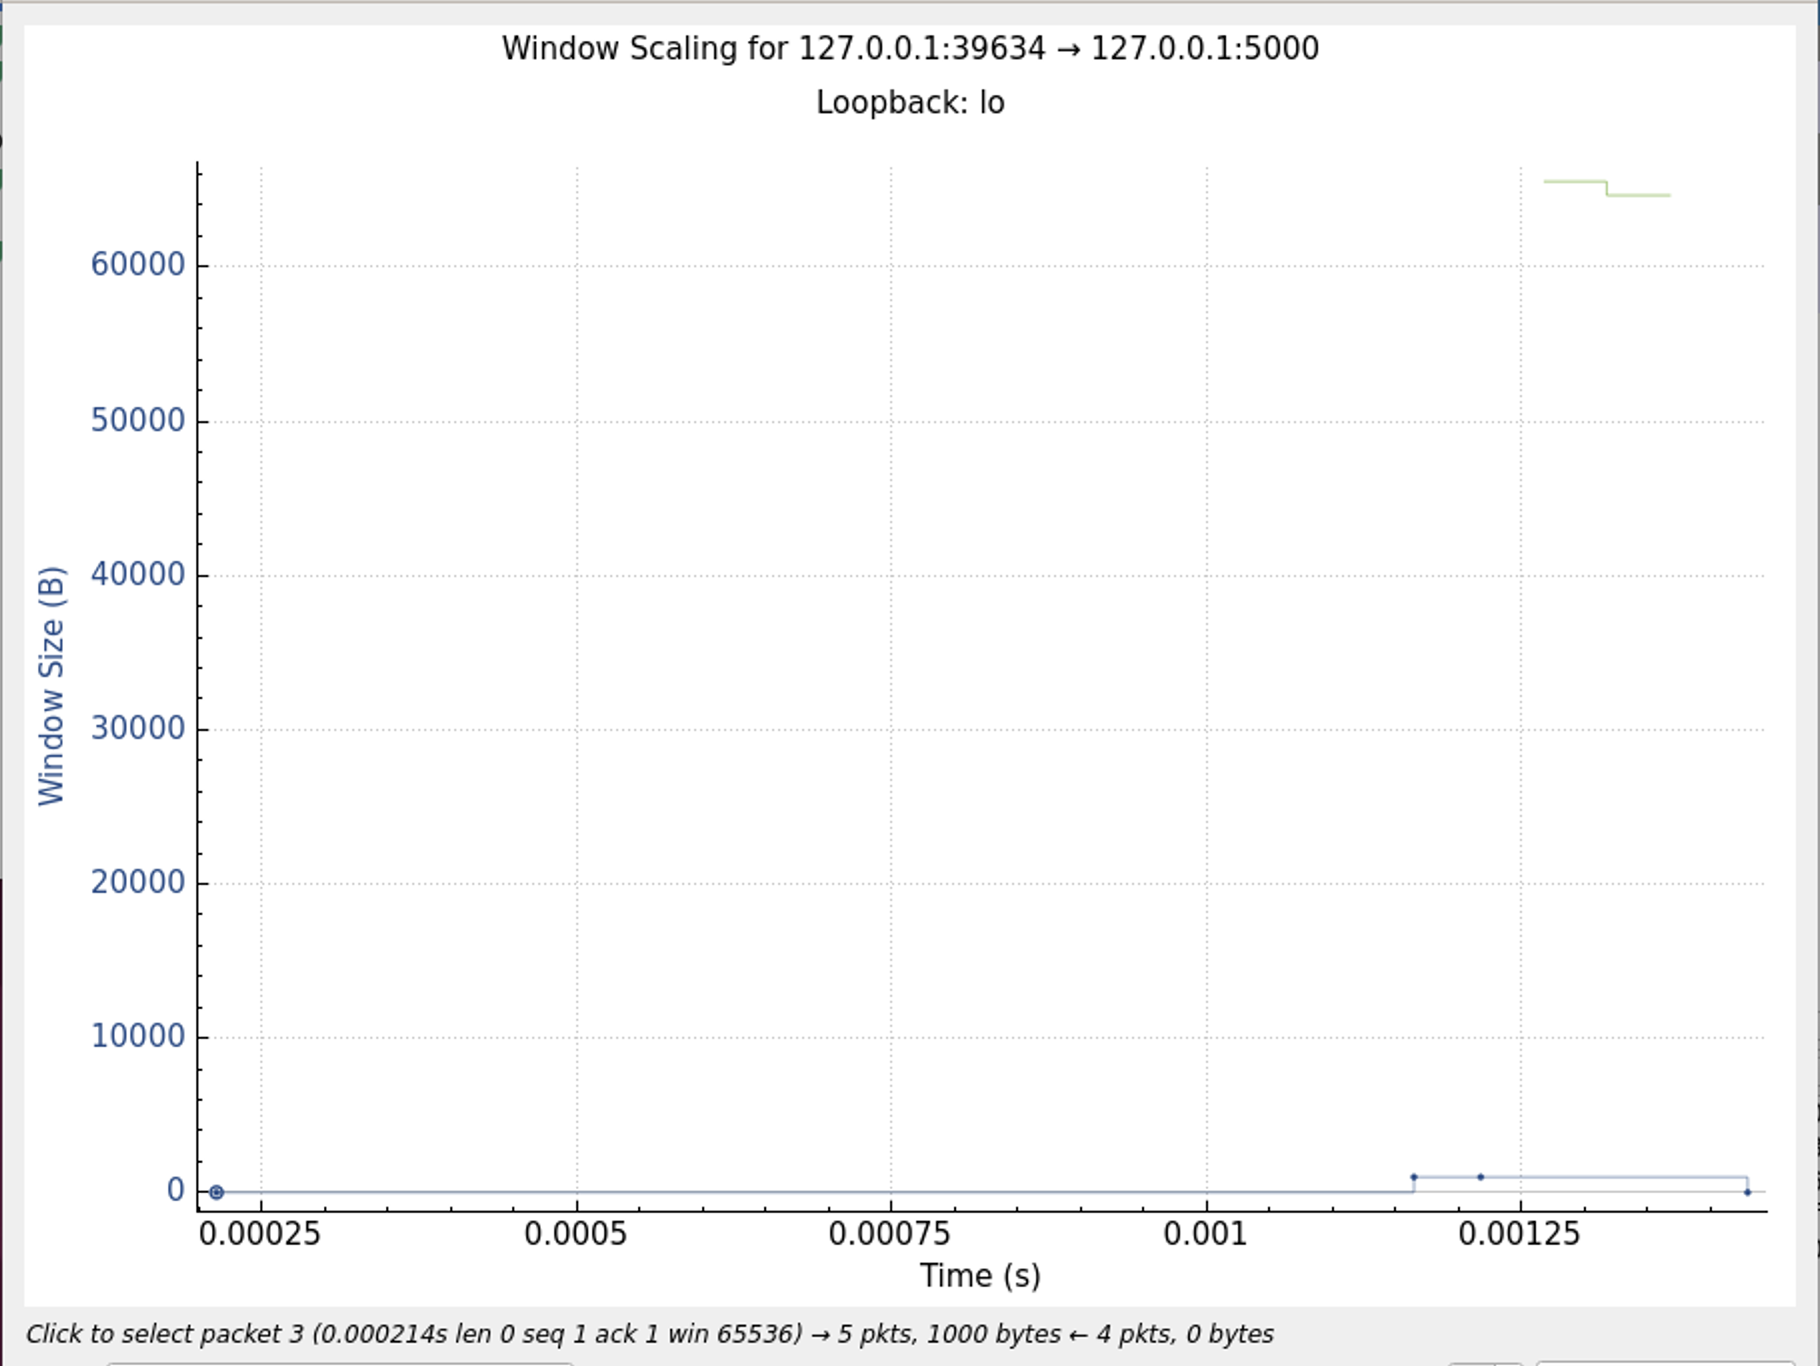
\includegraphics[width=\textwidth]{Pics/Cubic/r10mbit_s1000_ws}
        \caption{10 mbit rate 1kbit sent}
    \end{subfigure}
    \hfill
    \begin{subfigure}[b]{0.45\textwidth}
        \centering
        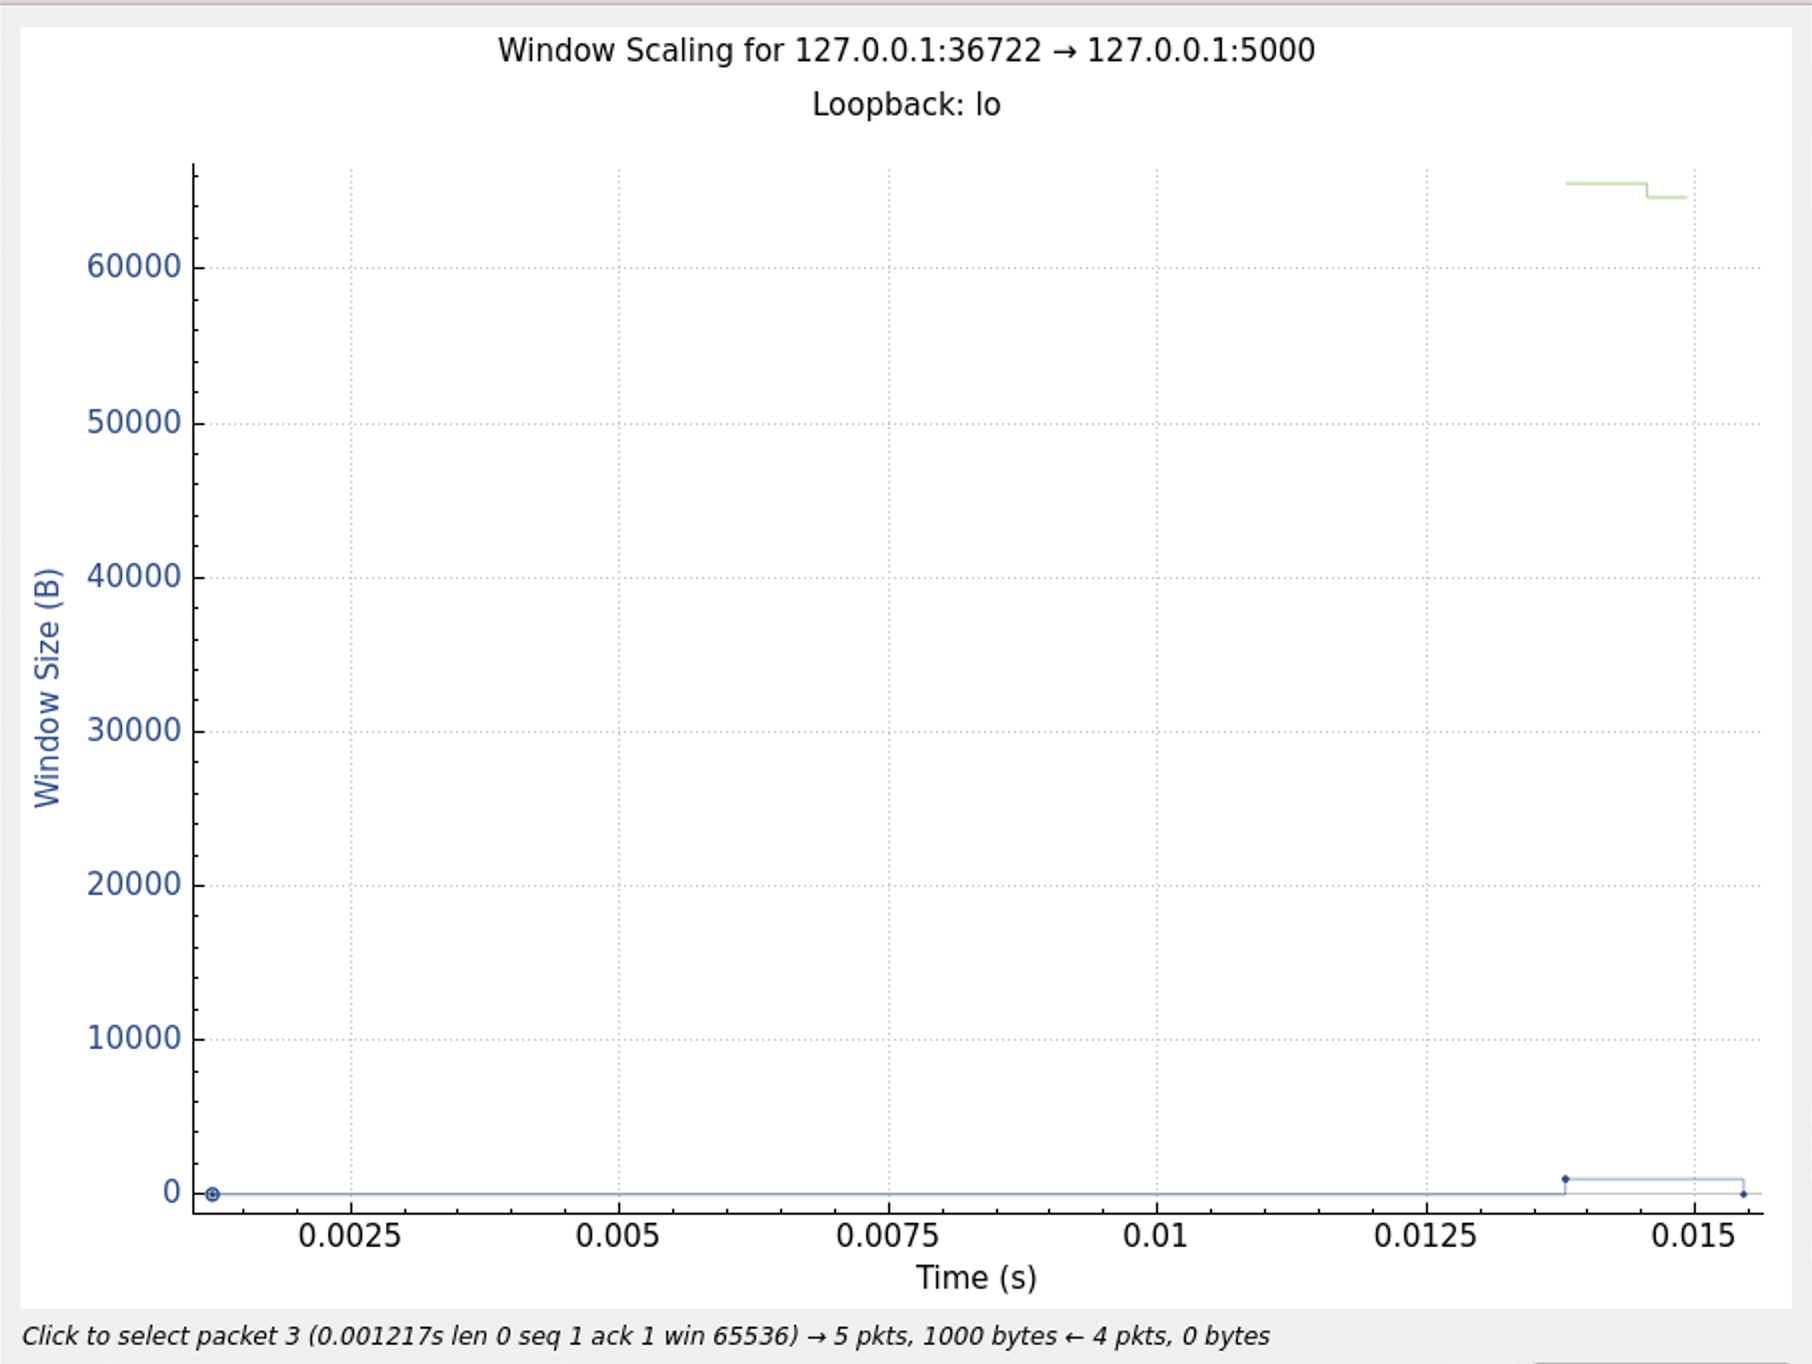
\includegraphics[width=\textwidth]{Pics/Cubic/r1mbit_s1000_ws}
        \caption{1 mbit rate 1kbit sent}
    \end{subfigure}
    \medskip

    \begin{subfigure}[b]{0.45\textwidth}
        \centering
        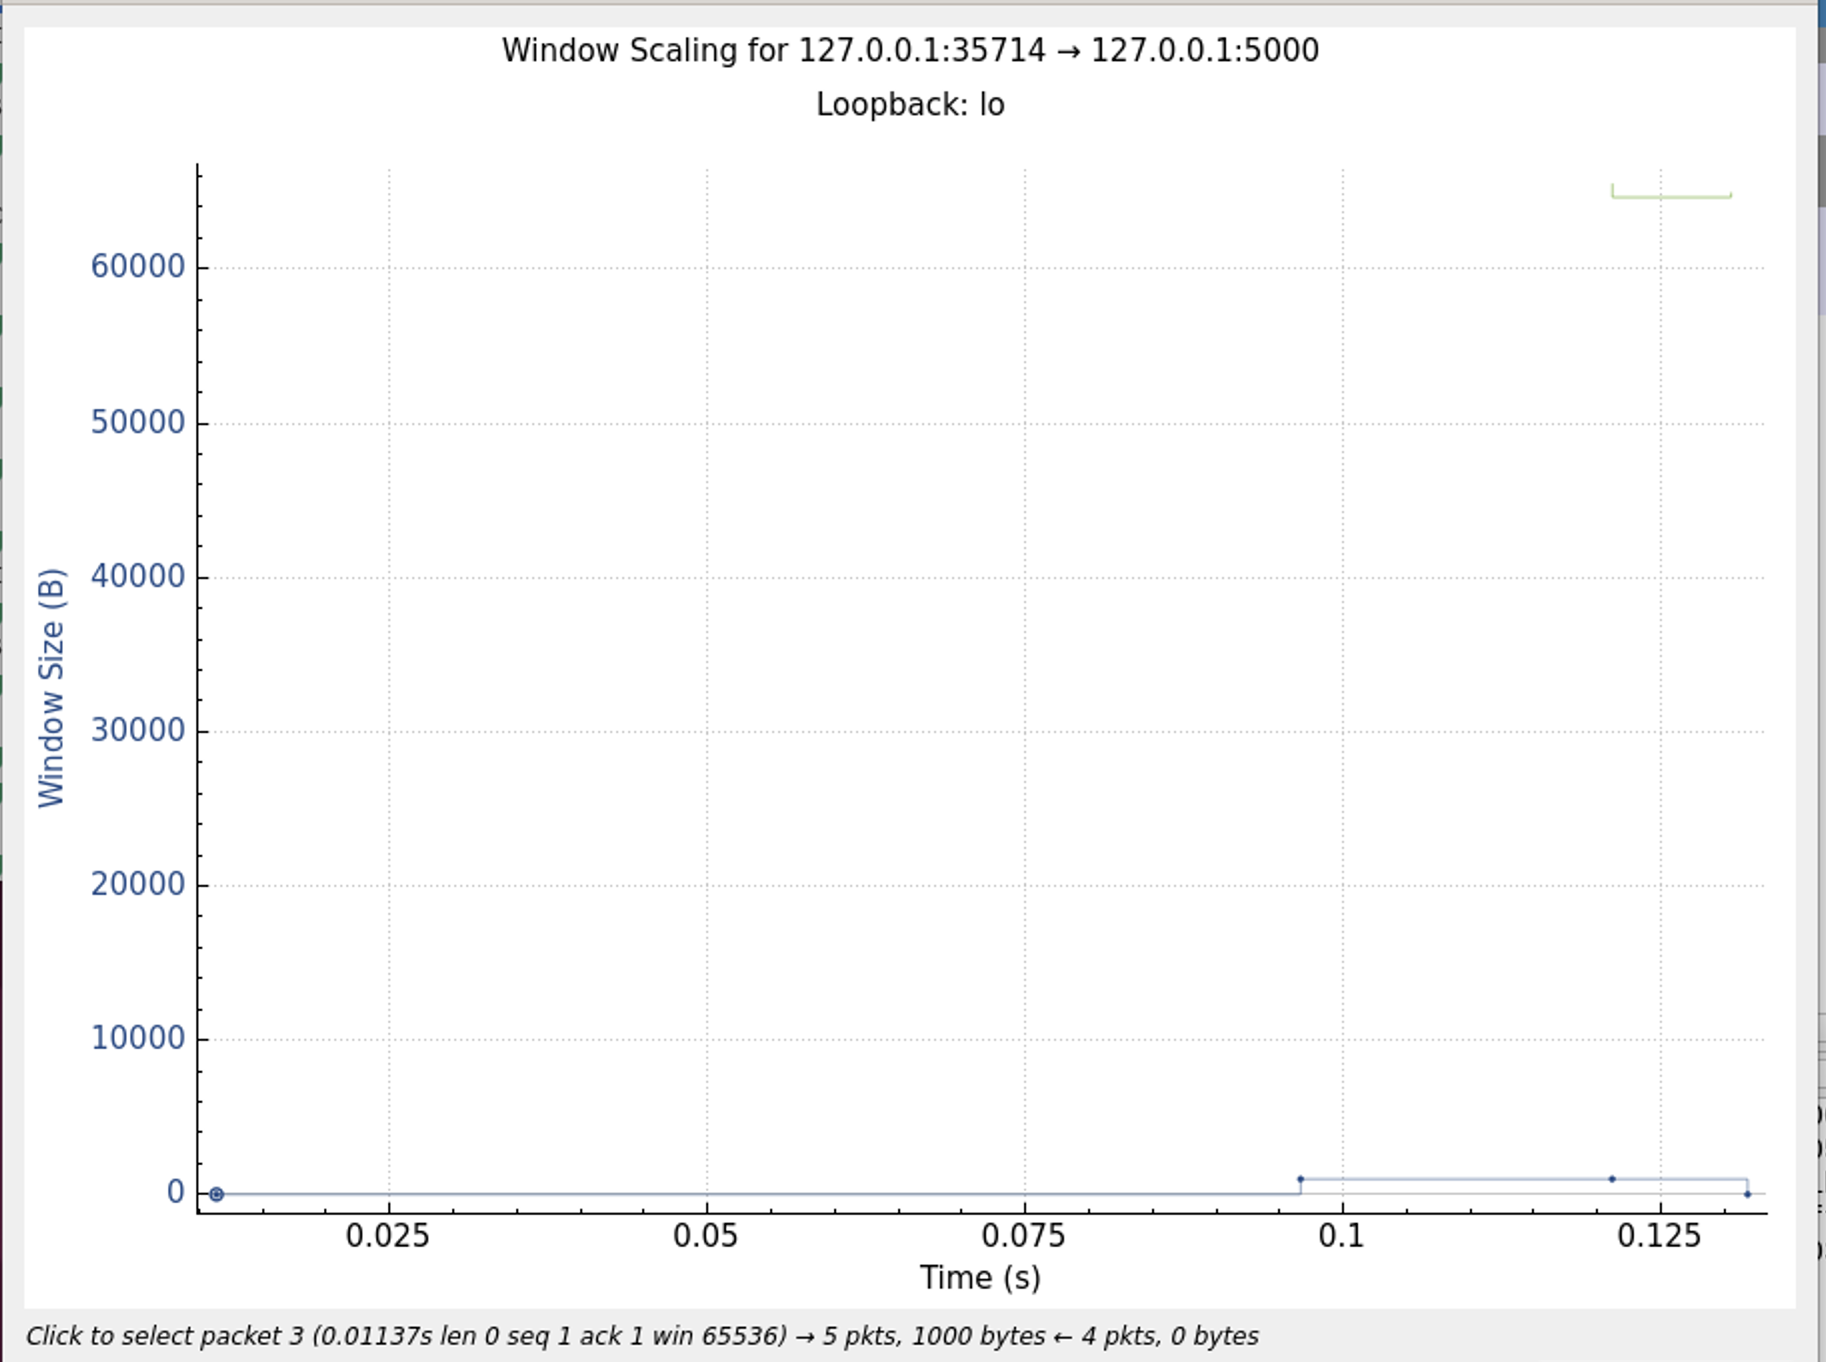
\includegraphics[width=\textwidth]{Pics/Cubic/r100kbit_s1000_ws}
        \caption{100 kbit rate 1kbit sent}
    \end{subfigure}
    \hfill
    \begin{subfigure}[b]{0.45\textwidth}
        \centering
        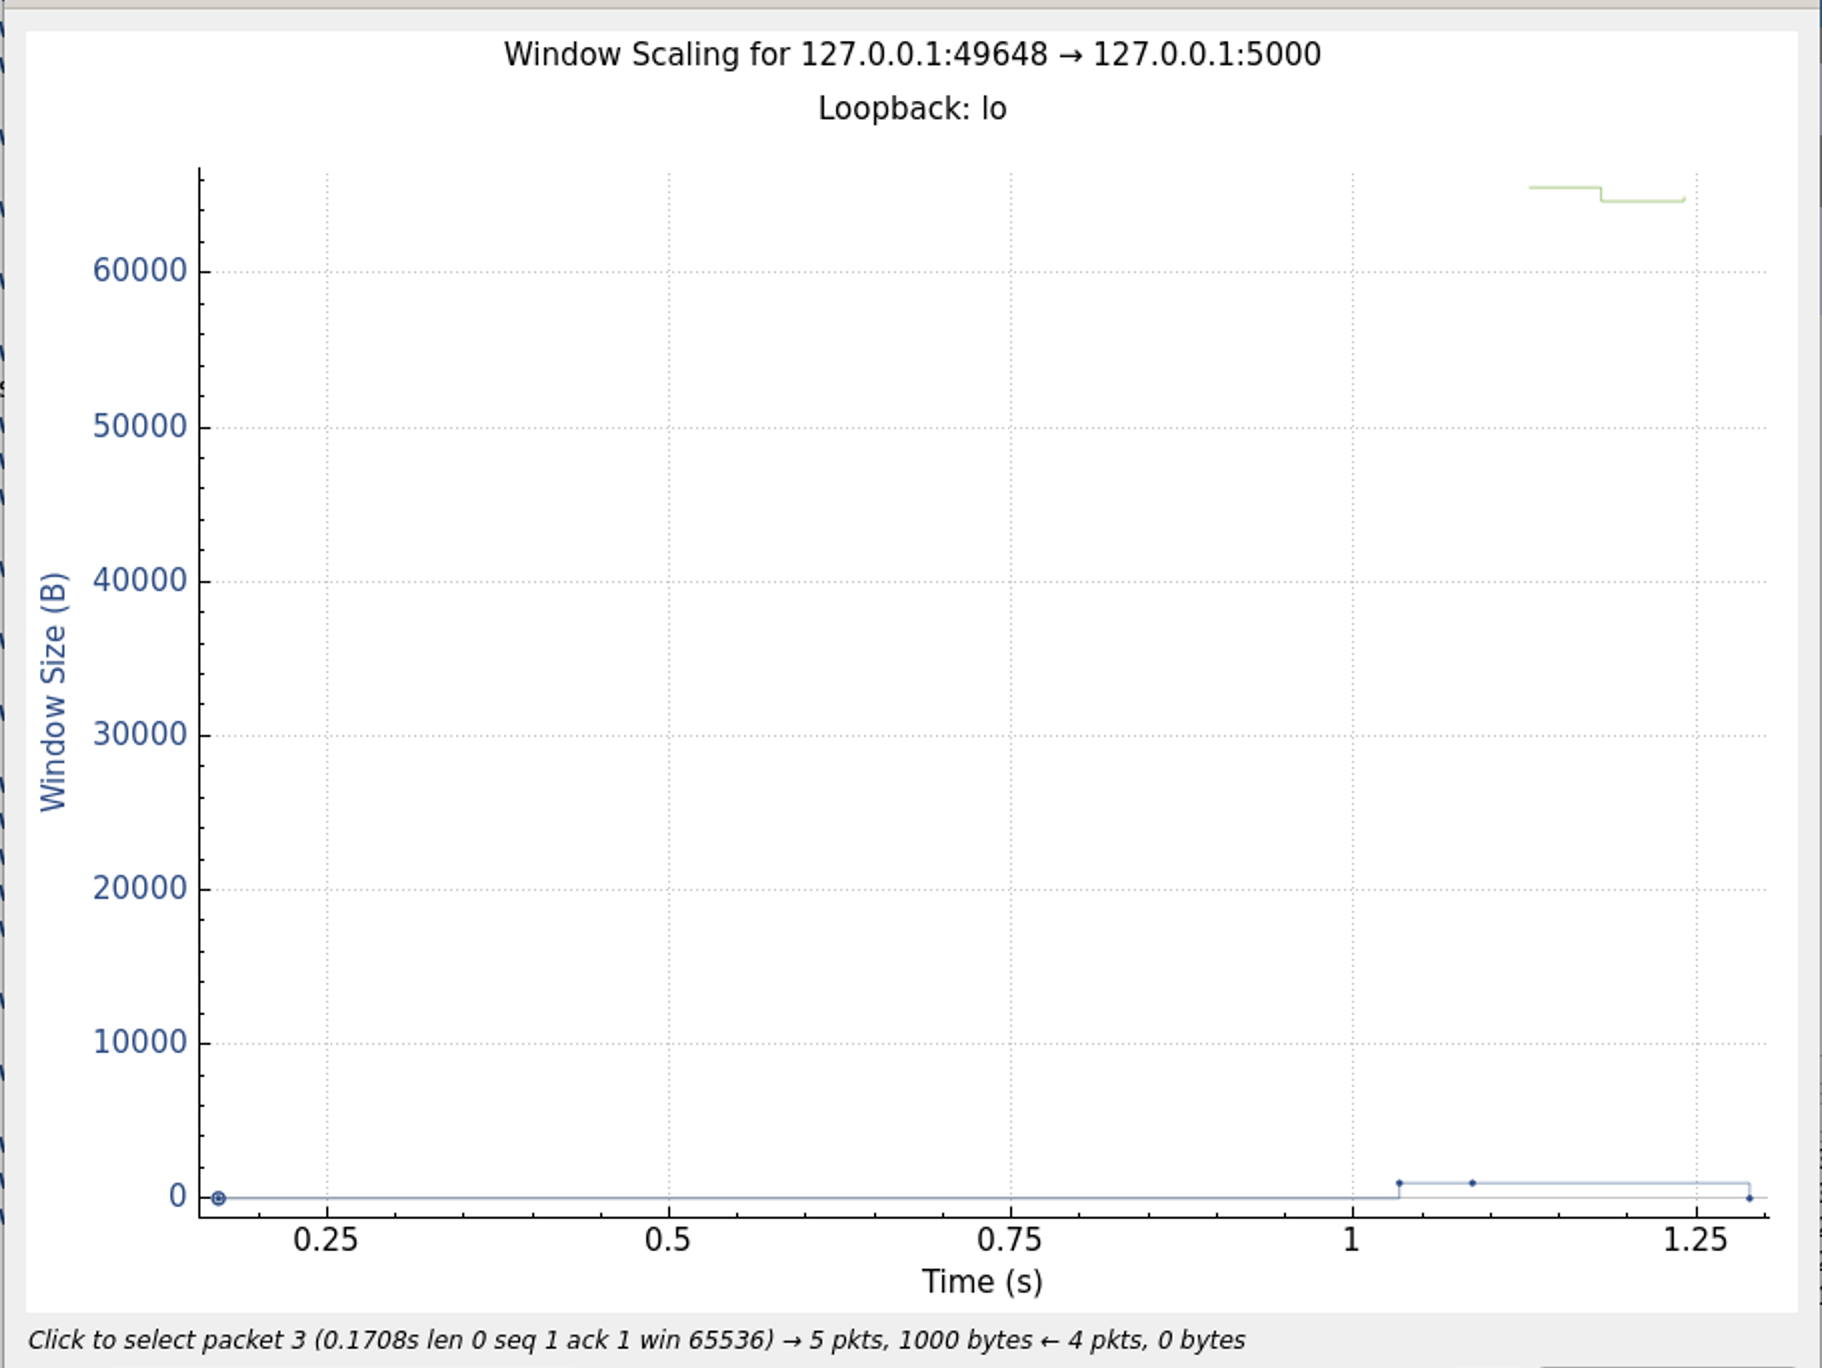
\includegraphics[width=\textwidth]{Pics/Cubic/r10kbit_s1000_ws}
        \caption{10 kbit rate 1kbit sent}
    \end{subfigure}
    \caption{Comparison of the window scaling for a total sent data of 1kb with 4 different rates}
    \label{fig:four_images}
\end{figure}

On the other hand, unsurprisingly, the round trip time was much more influenced by the change in rate even for small data sizes sent.\\
\begin{figure}[H]
    \centering
    \begin{subfigure}[b]{0.45\textwidth}
        \centering
        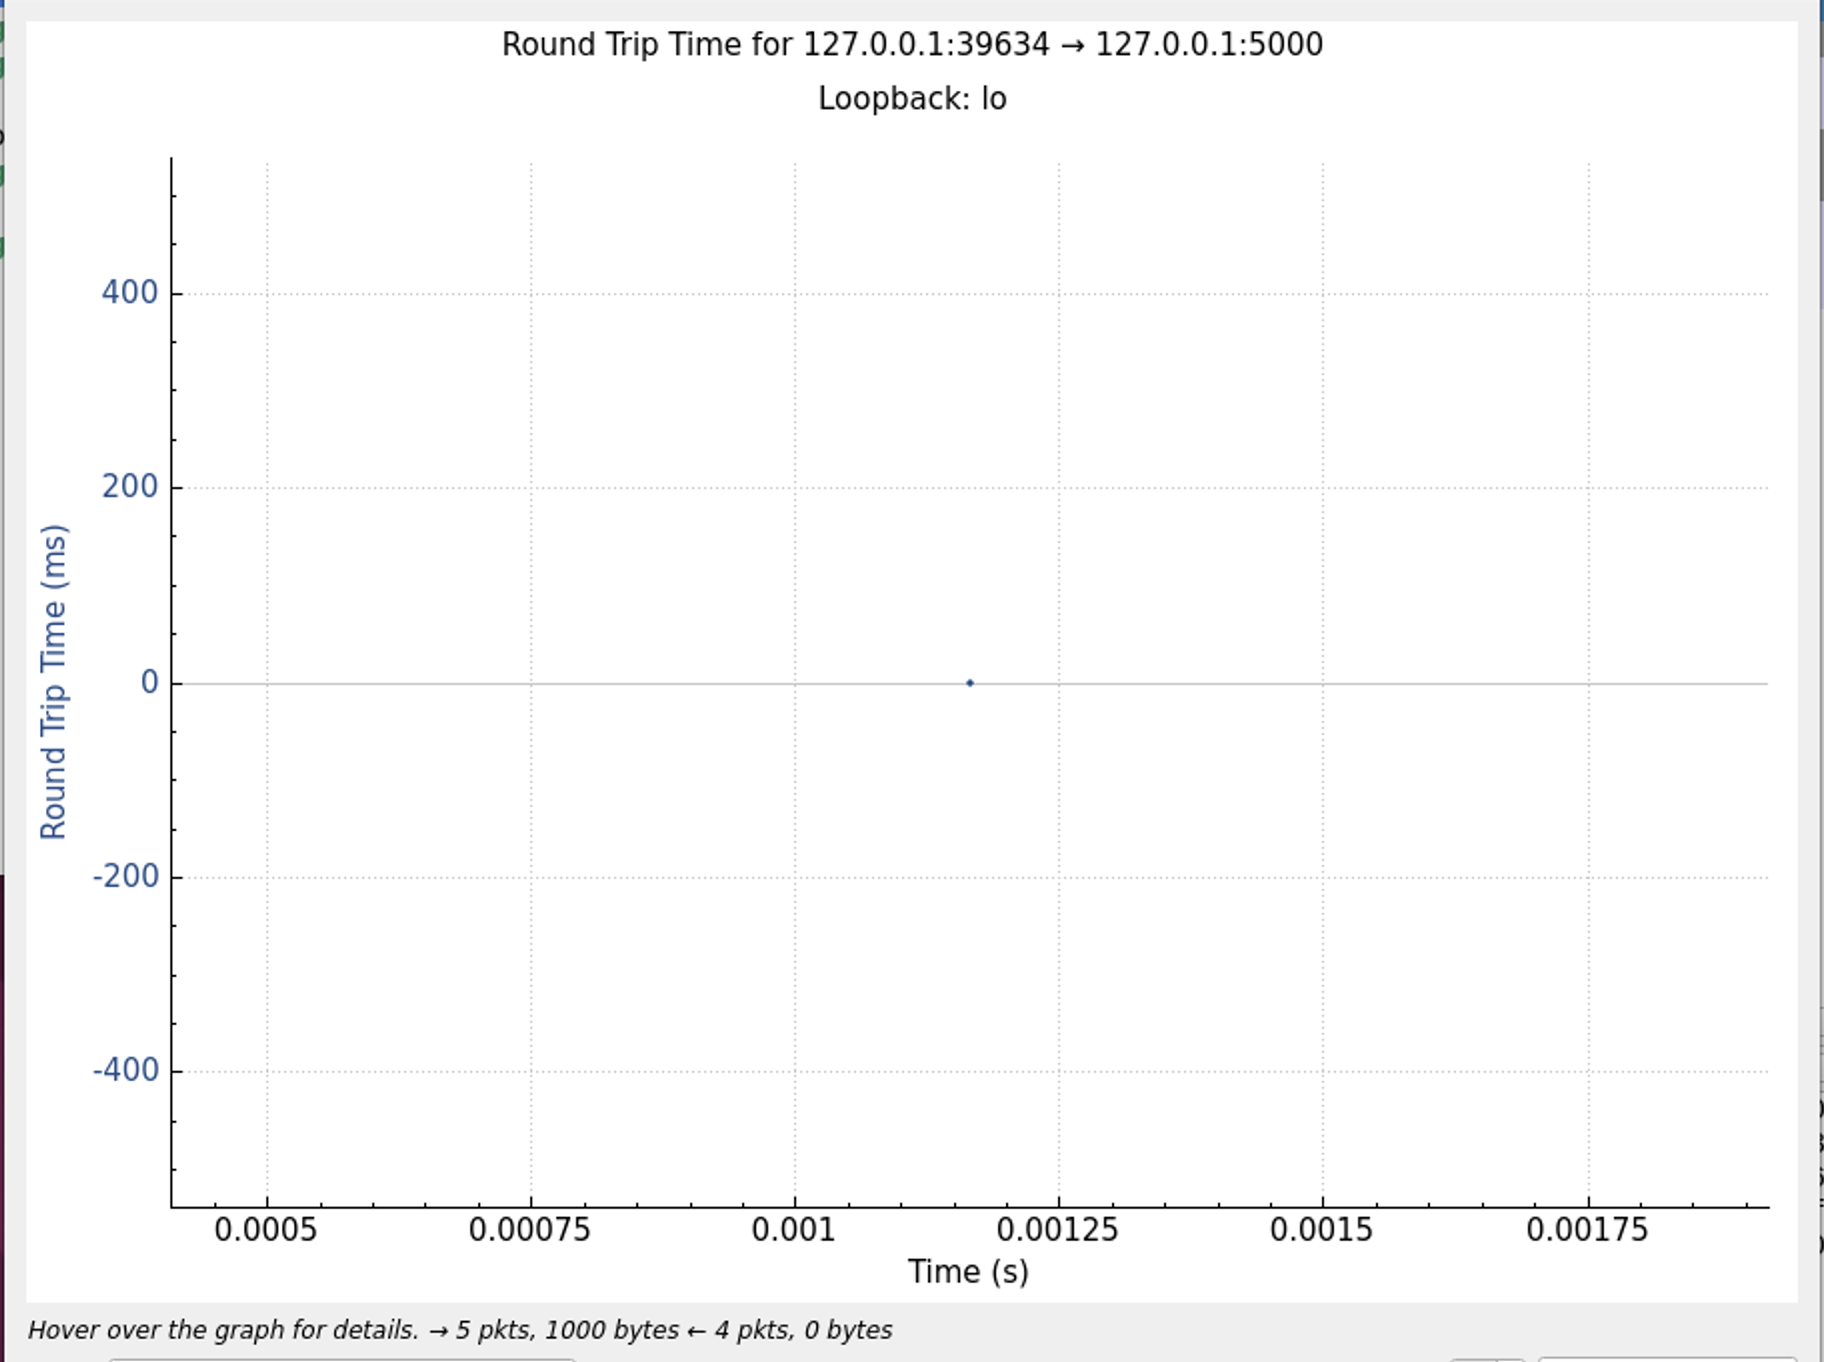
\includegraphics[width=\textwidth]{Pics/Cubic/r10mbit_s1000_rtt}
        \caption{10 mbit rate 1kbit sent}
    \end{subfigure}
    \hfill
    \begin{subfigure}[b]{0.45\textwidth}
        \centering
        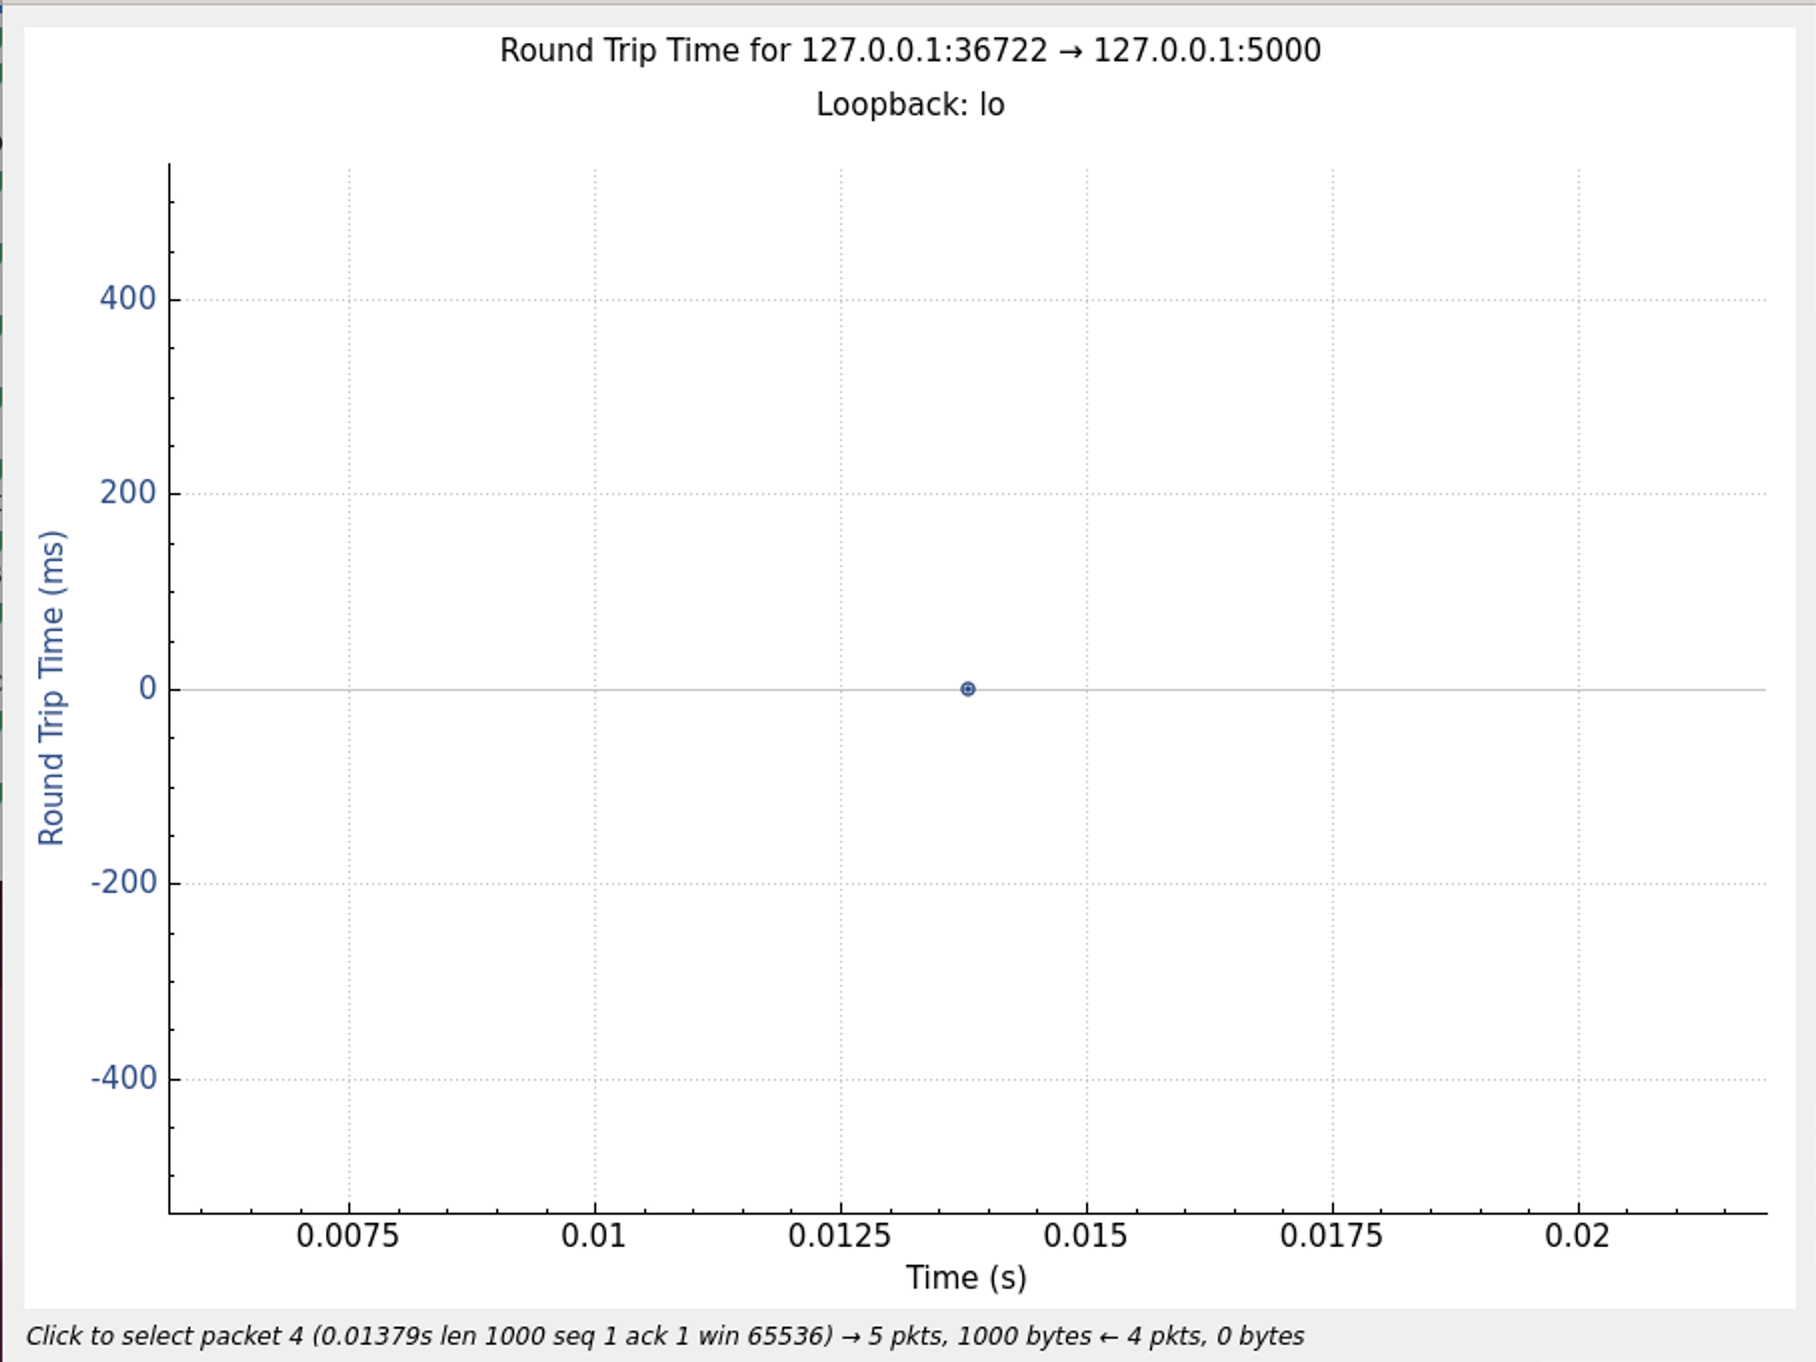
\includegraphics[width=\textwidth]{Pics/Cubic/r1mbit_s1000_rtt}
        \caption{1 mbit rate 1kbit sent}
    \end{subfigure}
    \medskip

    \begin{subfigure}[b]{0.45\textwidth}
        \centering
        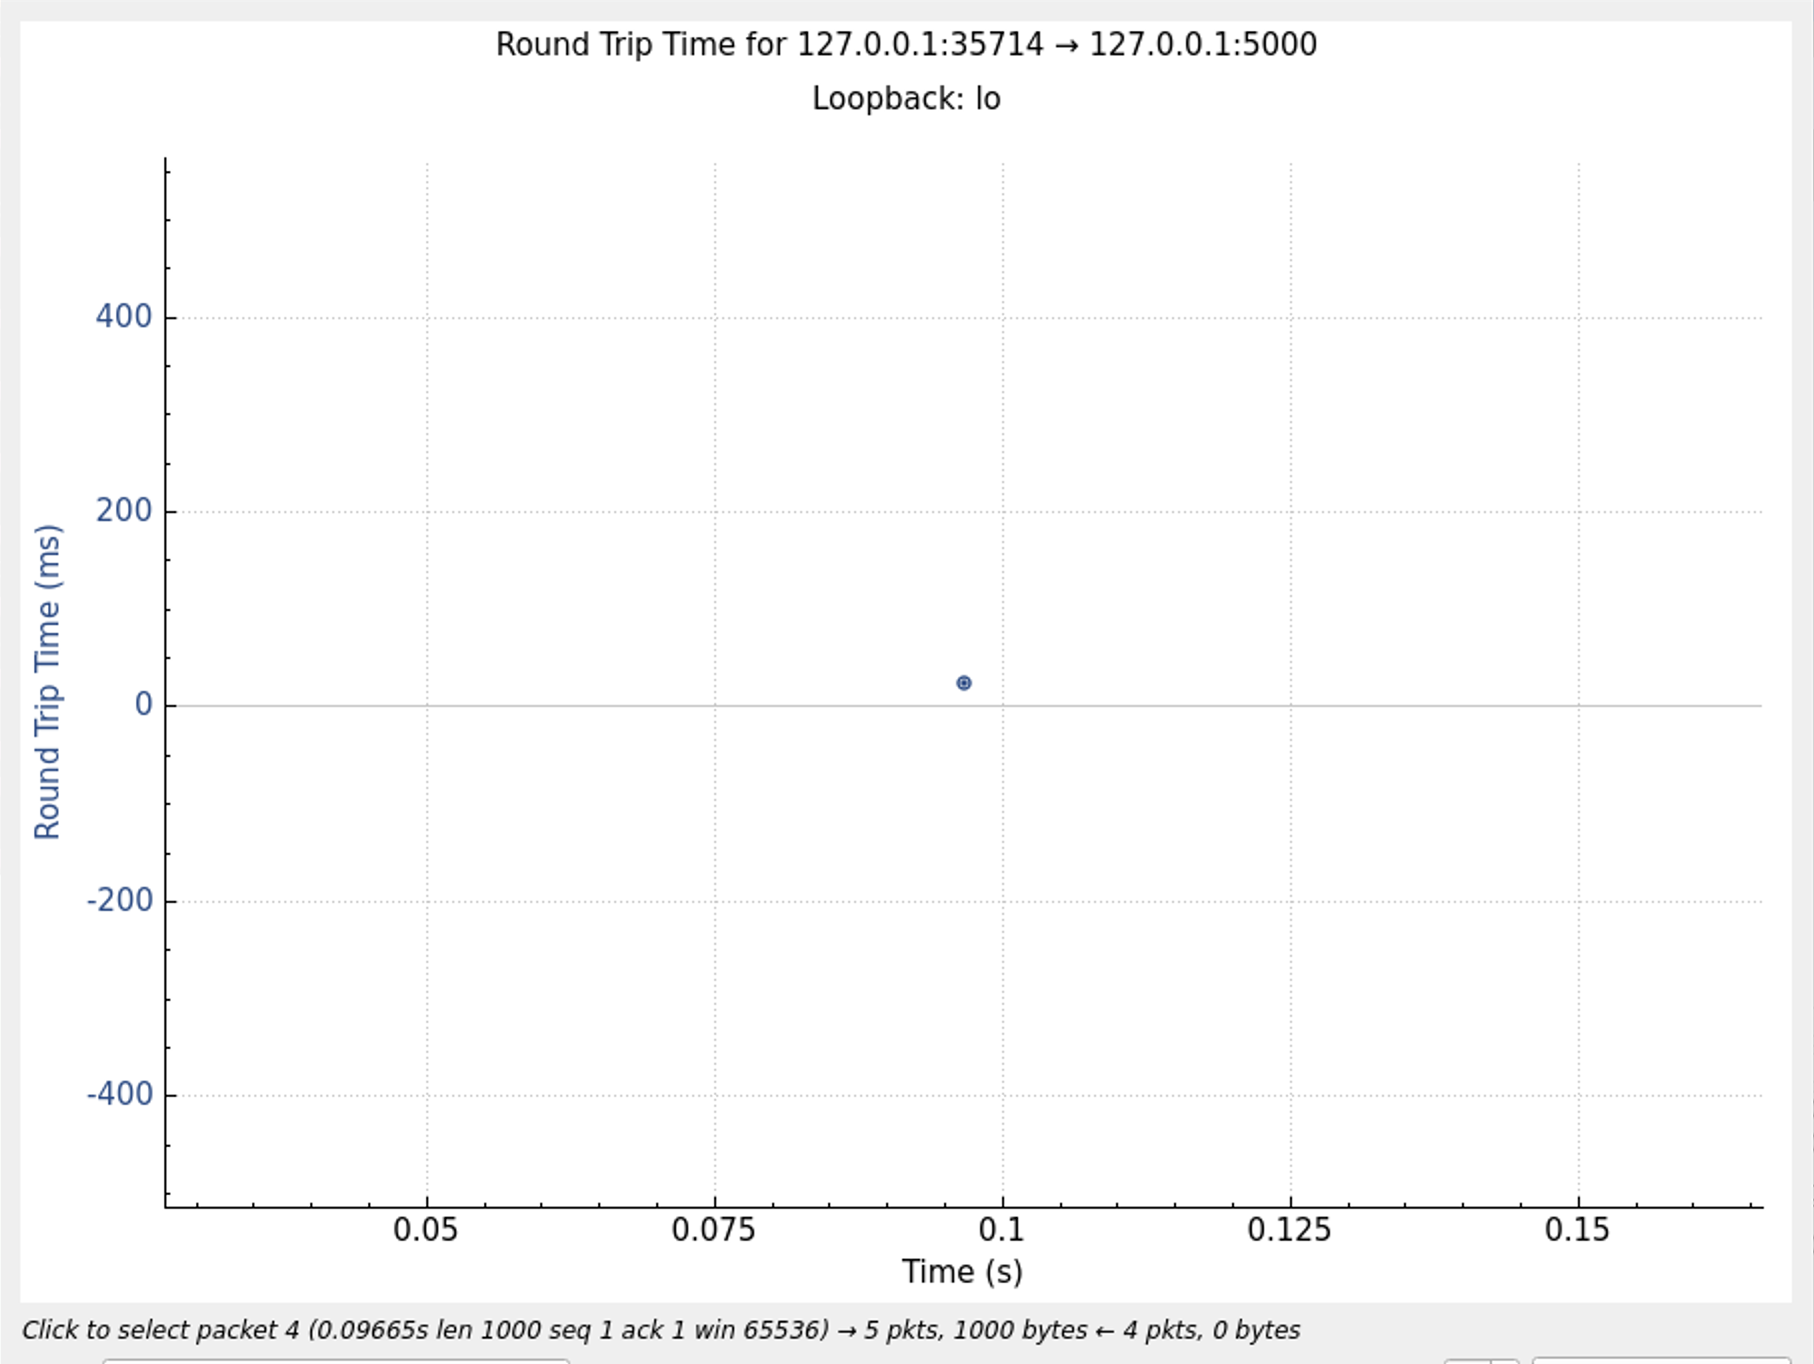
\includegraphics[width=\textwidth]{Pics/Cubic/r100kbit_s1000_rtt}
        \caption{100 kbit rate 1kbit sent}
    \end{subfigure}
    \hfill
    \begin{subfigure}[b]{0.45\textwidth}
        \centering
        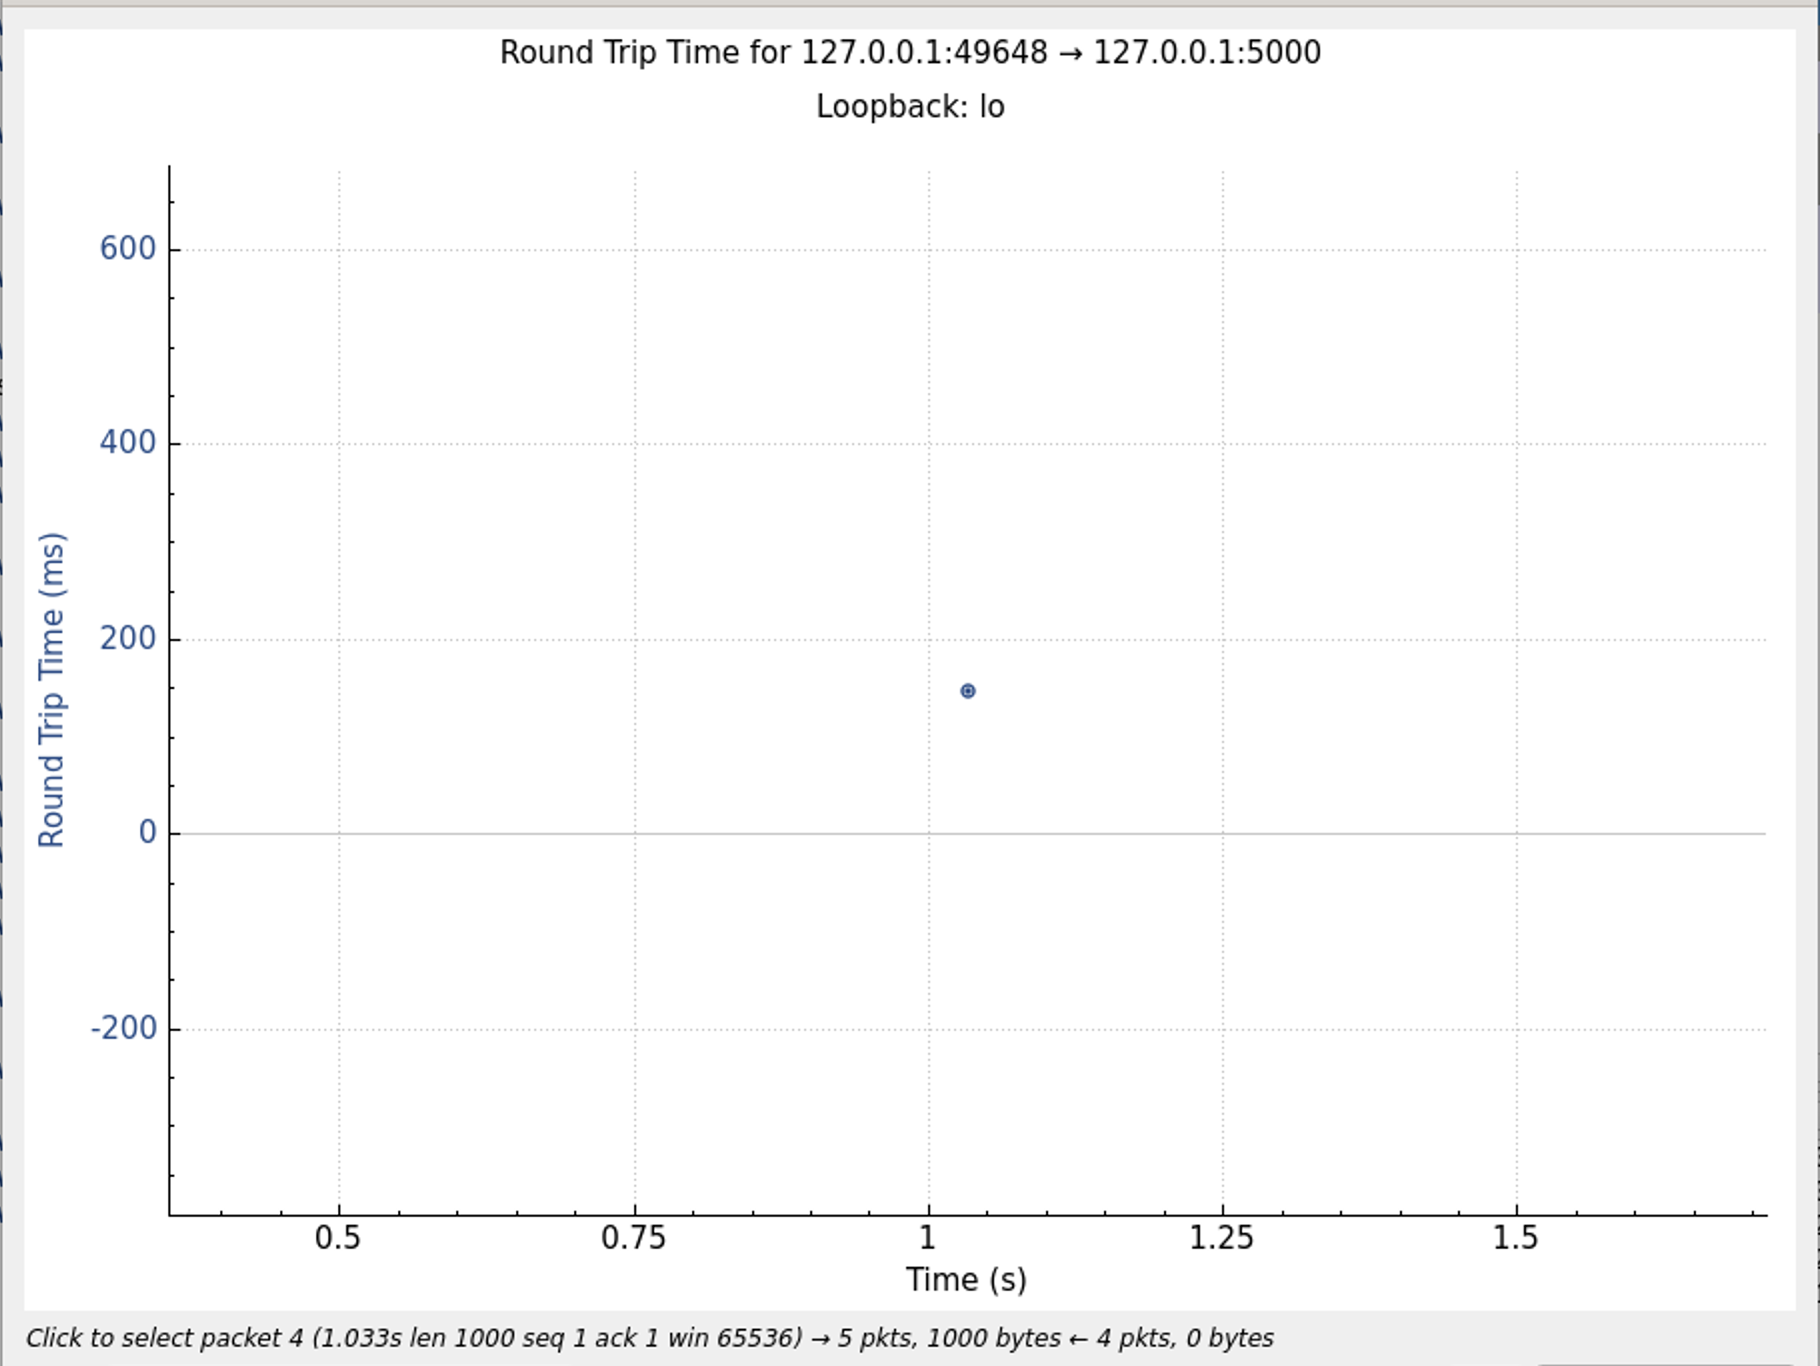
\includegraphics[width=\textwidth]{Pics/Cubic/r10kbit_s1000_rtt}
        \caption{10 kbit rate 1kbit sent}
    \end{subfigure}
    \caption{Comparison of the round trip time for 1kbit of data sent with different rate limits.}
    \label{fig:four_images}
\end{figure}

At a data sent size of 100kbit it starts to become visible the actual development of the window scaling through time. We can see, especially at lower rates, some moments in which the window scaling lowers drastically to then go back up.

\begin{figure}[H]
    \centering
    \begin{subfigure}[b]{0.45\textwidth}
        \centering
        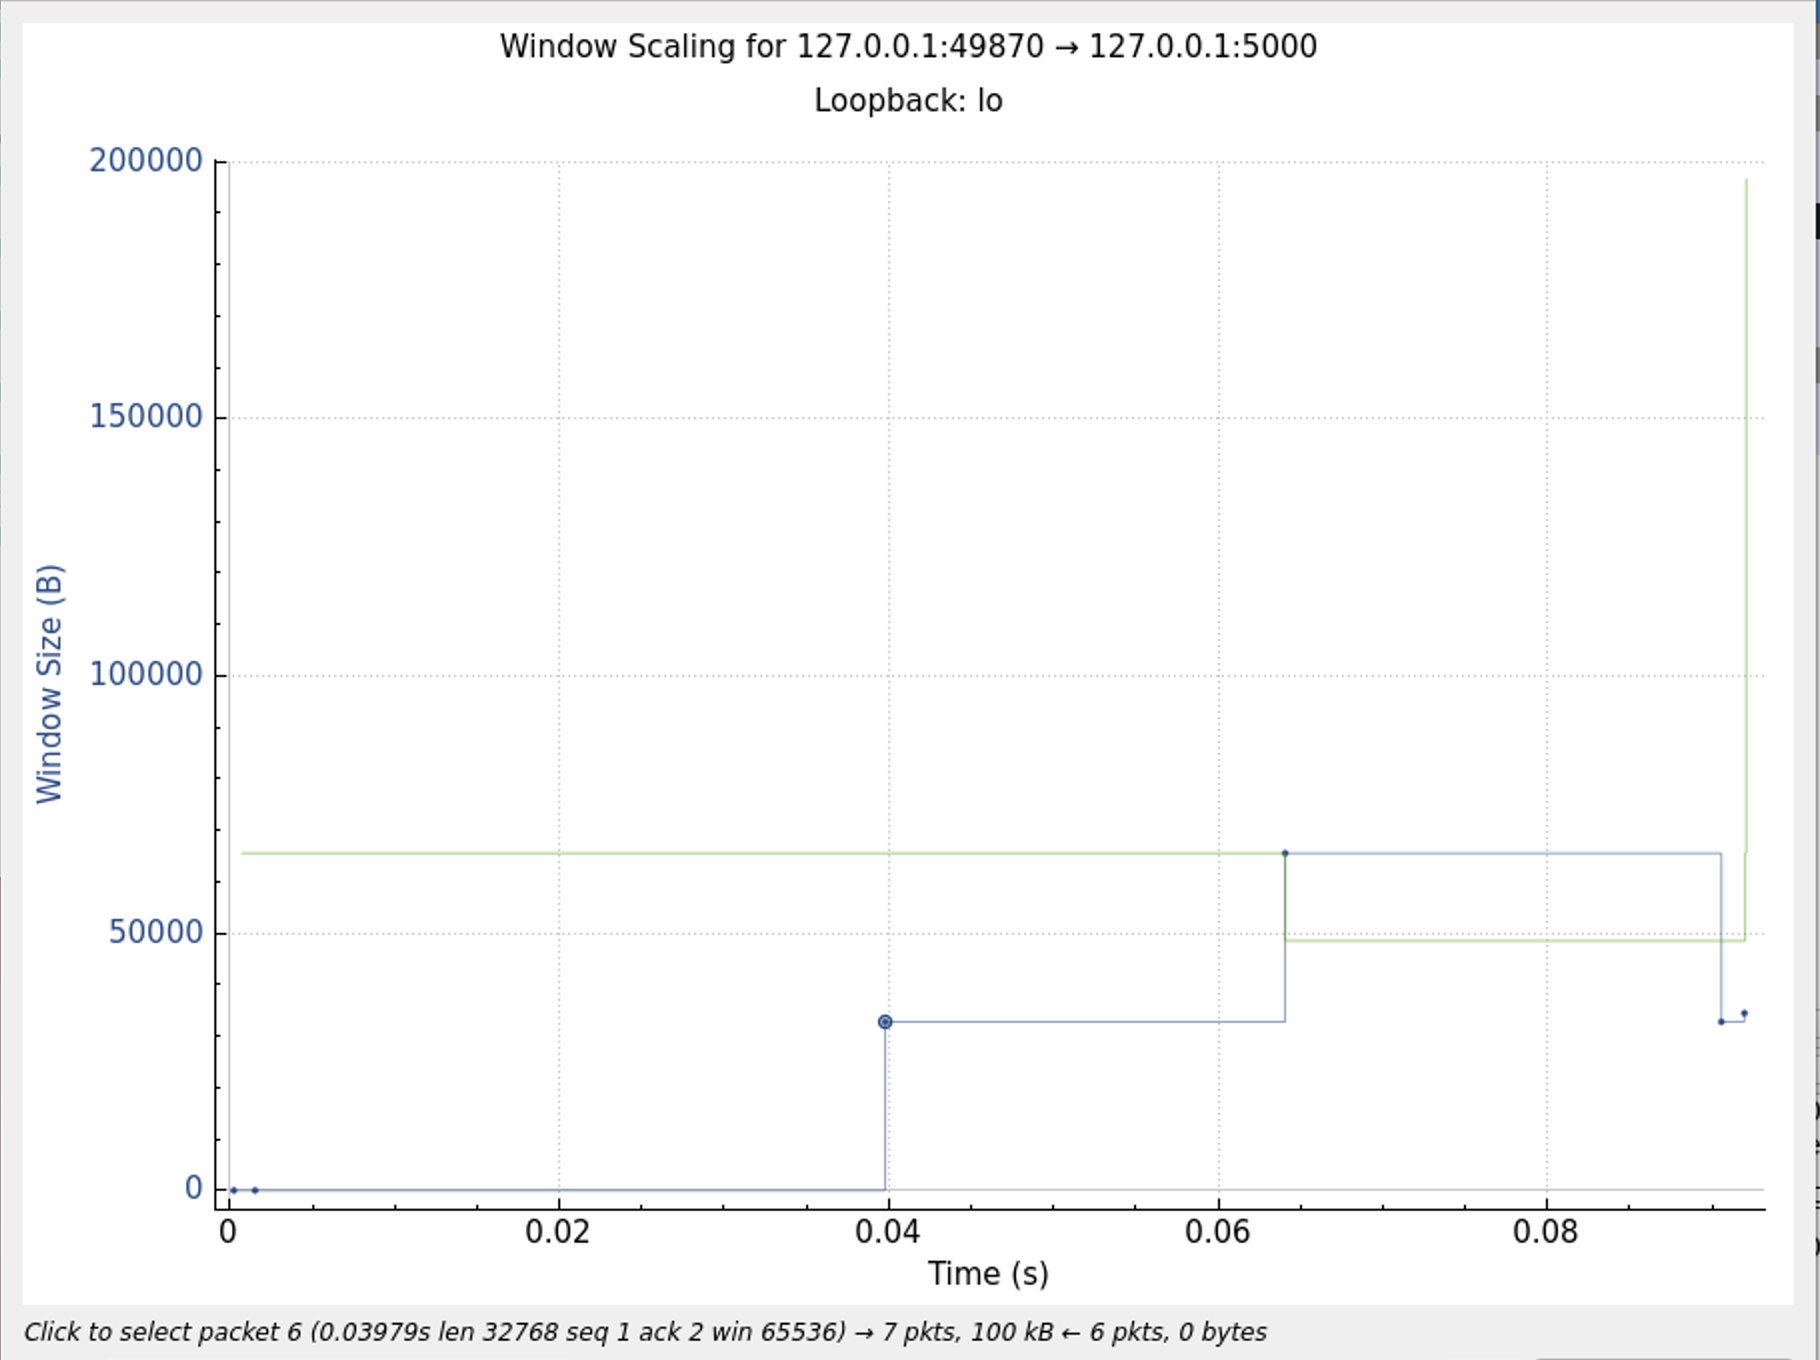
\includegraphics[width=\textwidth]{Pics/Cubic/r10mbit_s100k_ws}
        \caption{10 mbit rate}
    \end{subfigure}
    \hfill
    \begin{subfigure}[b]{0.45\textwidth}
        \centering
        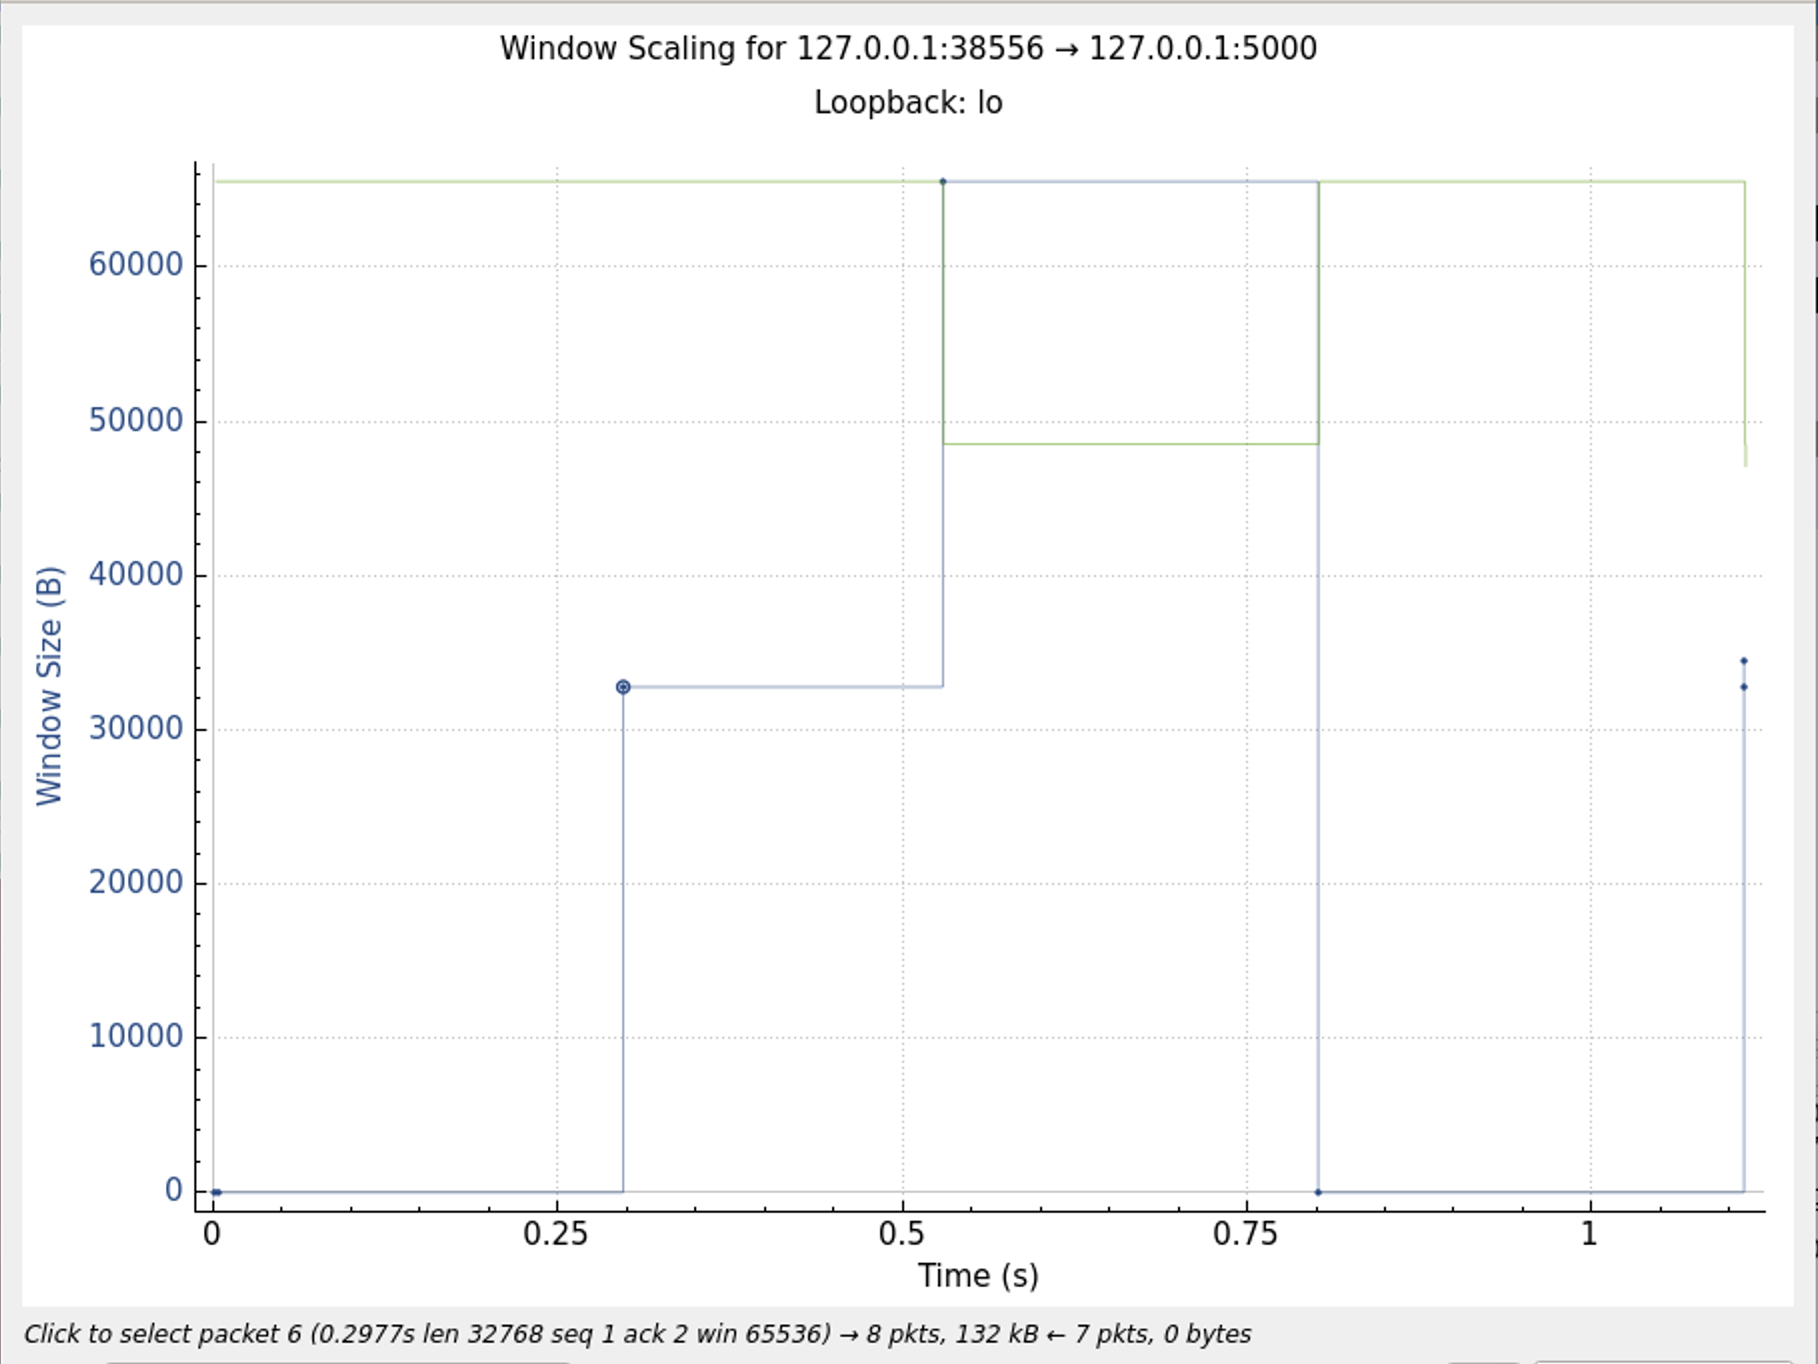
\includegraphics[width=\textwidth]{Pics/Cubic/r1mbit_s100k_ws}
        \caption{1 mbit rate }
    \end{subfigure}
    \medskip

    \begin{subfigure}[b]{0.45\textwidth}
        \centering
        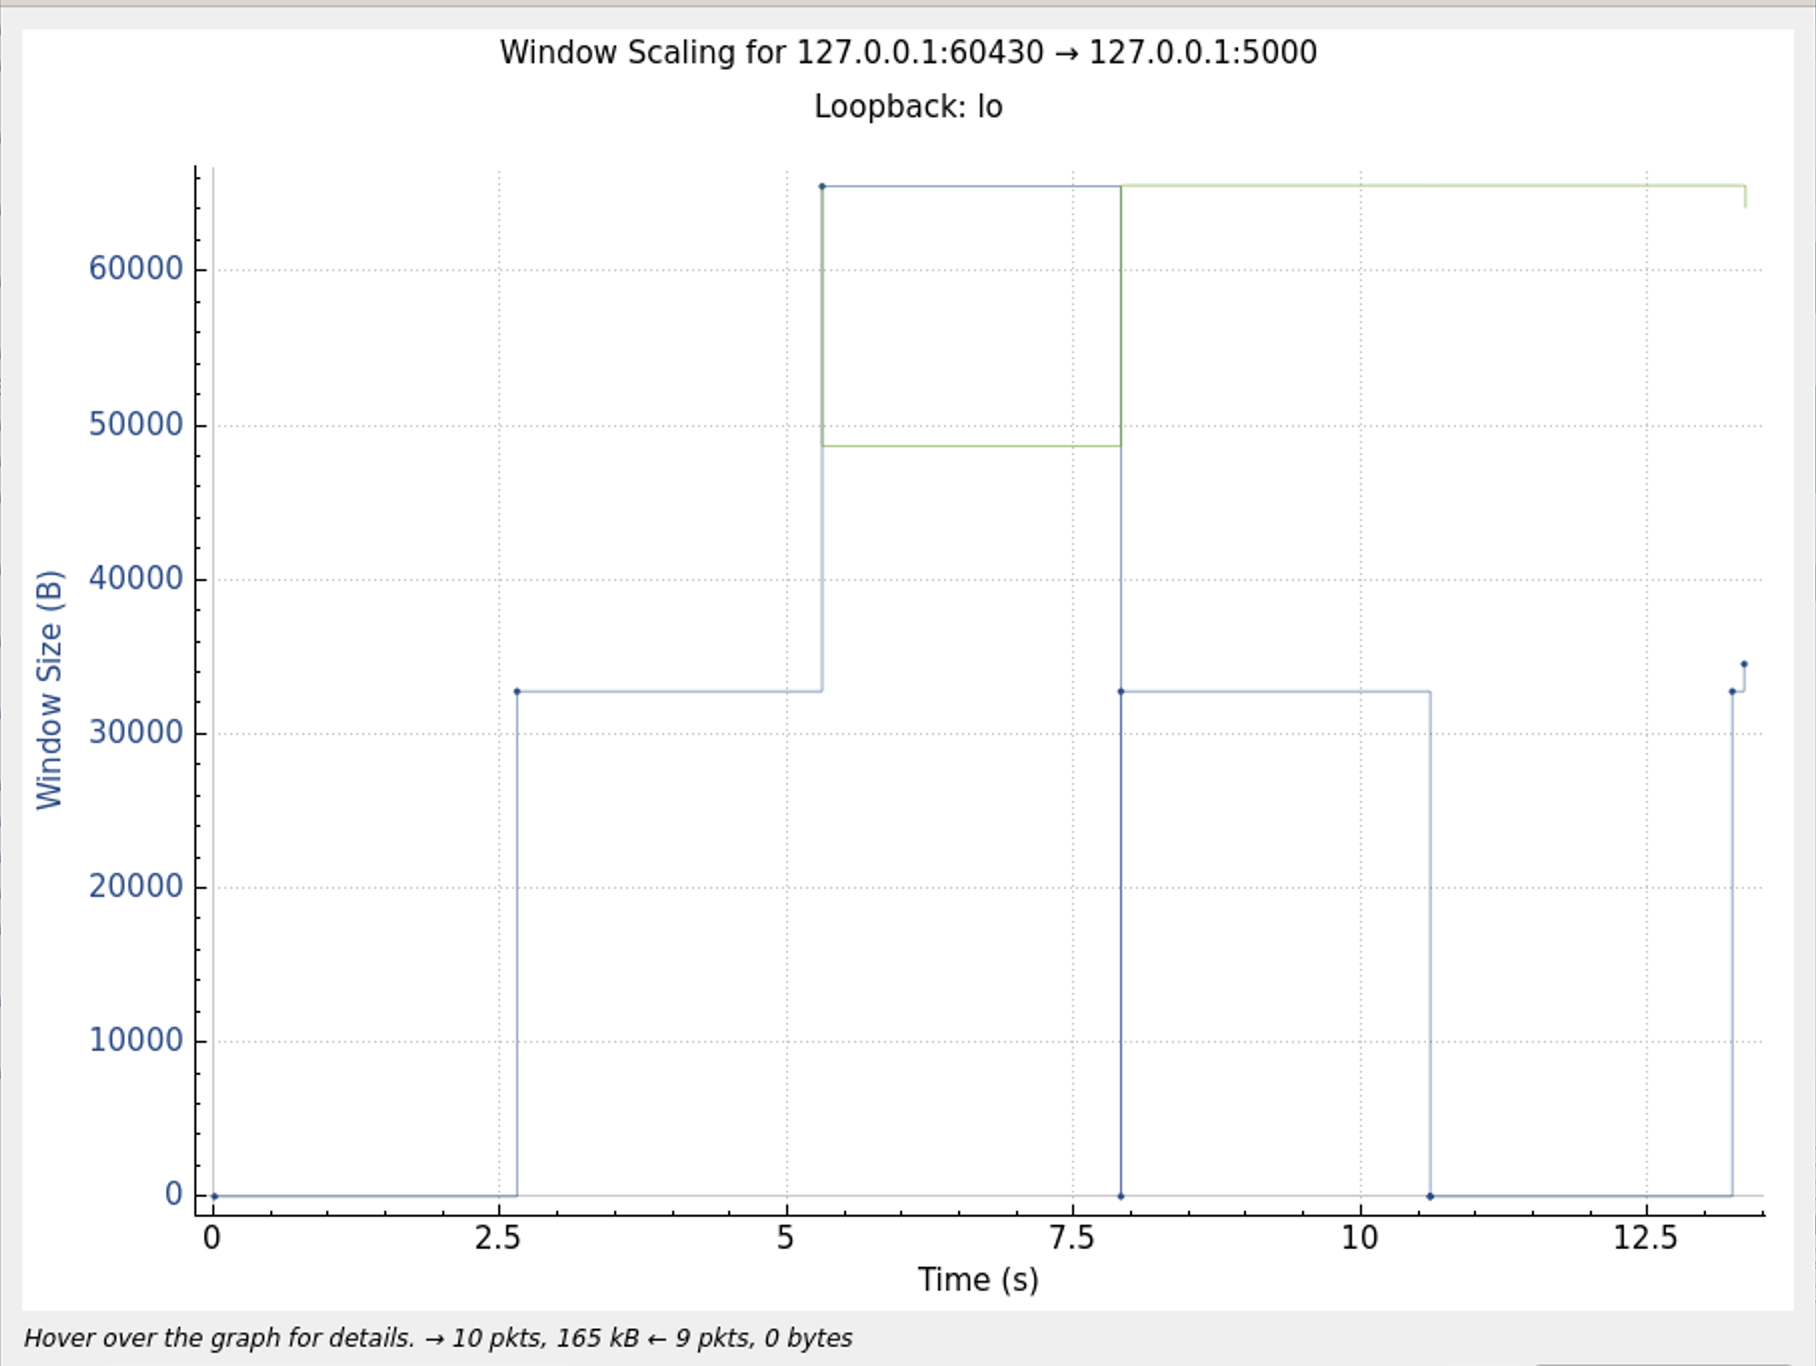
\includegraphics[width=\textwidth]{Pics/Cubic/r100kbit_s100k_ws}
        \caption{100 kbit rate}
    \end{subfigure}
    \hfill
    \begin{subfigure}[b]{0.45\textwidth}
        \centering
        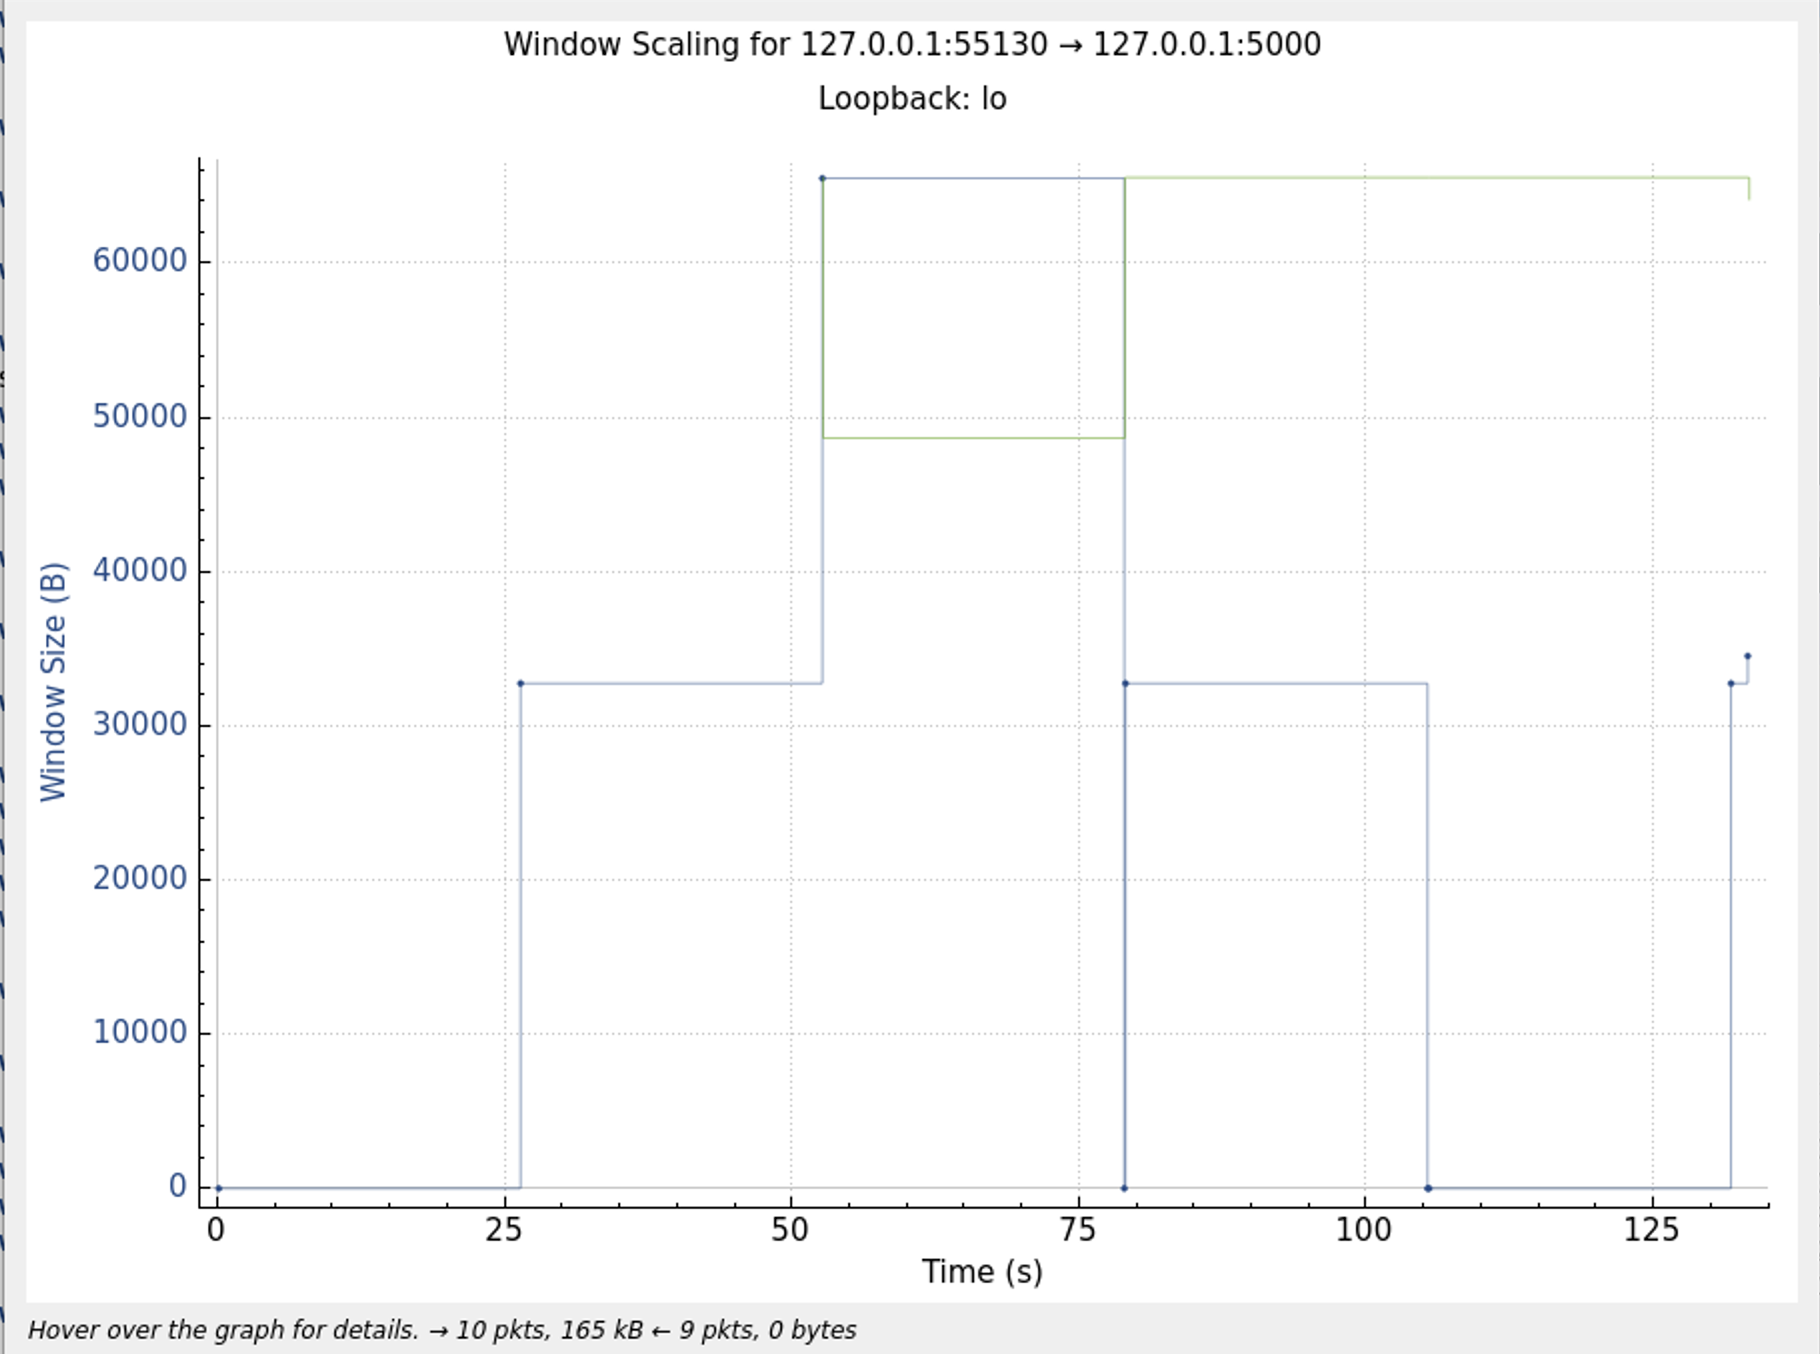
\includegraphics[width=\textwidth]{Pics/Cubic/r10kbit_s100kbit_ws}
        \caption{10 kbit rate}
    \end{subfigure}
    \caption{Comparison of the window scaling for 100kbit of data sent with different rate limits.}
    \label{fig:four_images}
\end{figure}

And at this size the throughput changes are also visible clearly. Especially for rates of 100kbit and 10kbit we can clearly see a regular pattern forming in the throughput. It alternates between very high spurts and moments of inactivity.
\begin{figure}[H]
    \centering
    \begin{subfigure}[b]{0.45\textwidth}
        \centering
        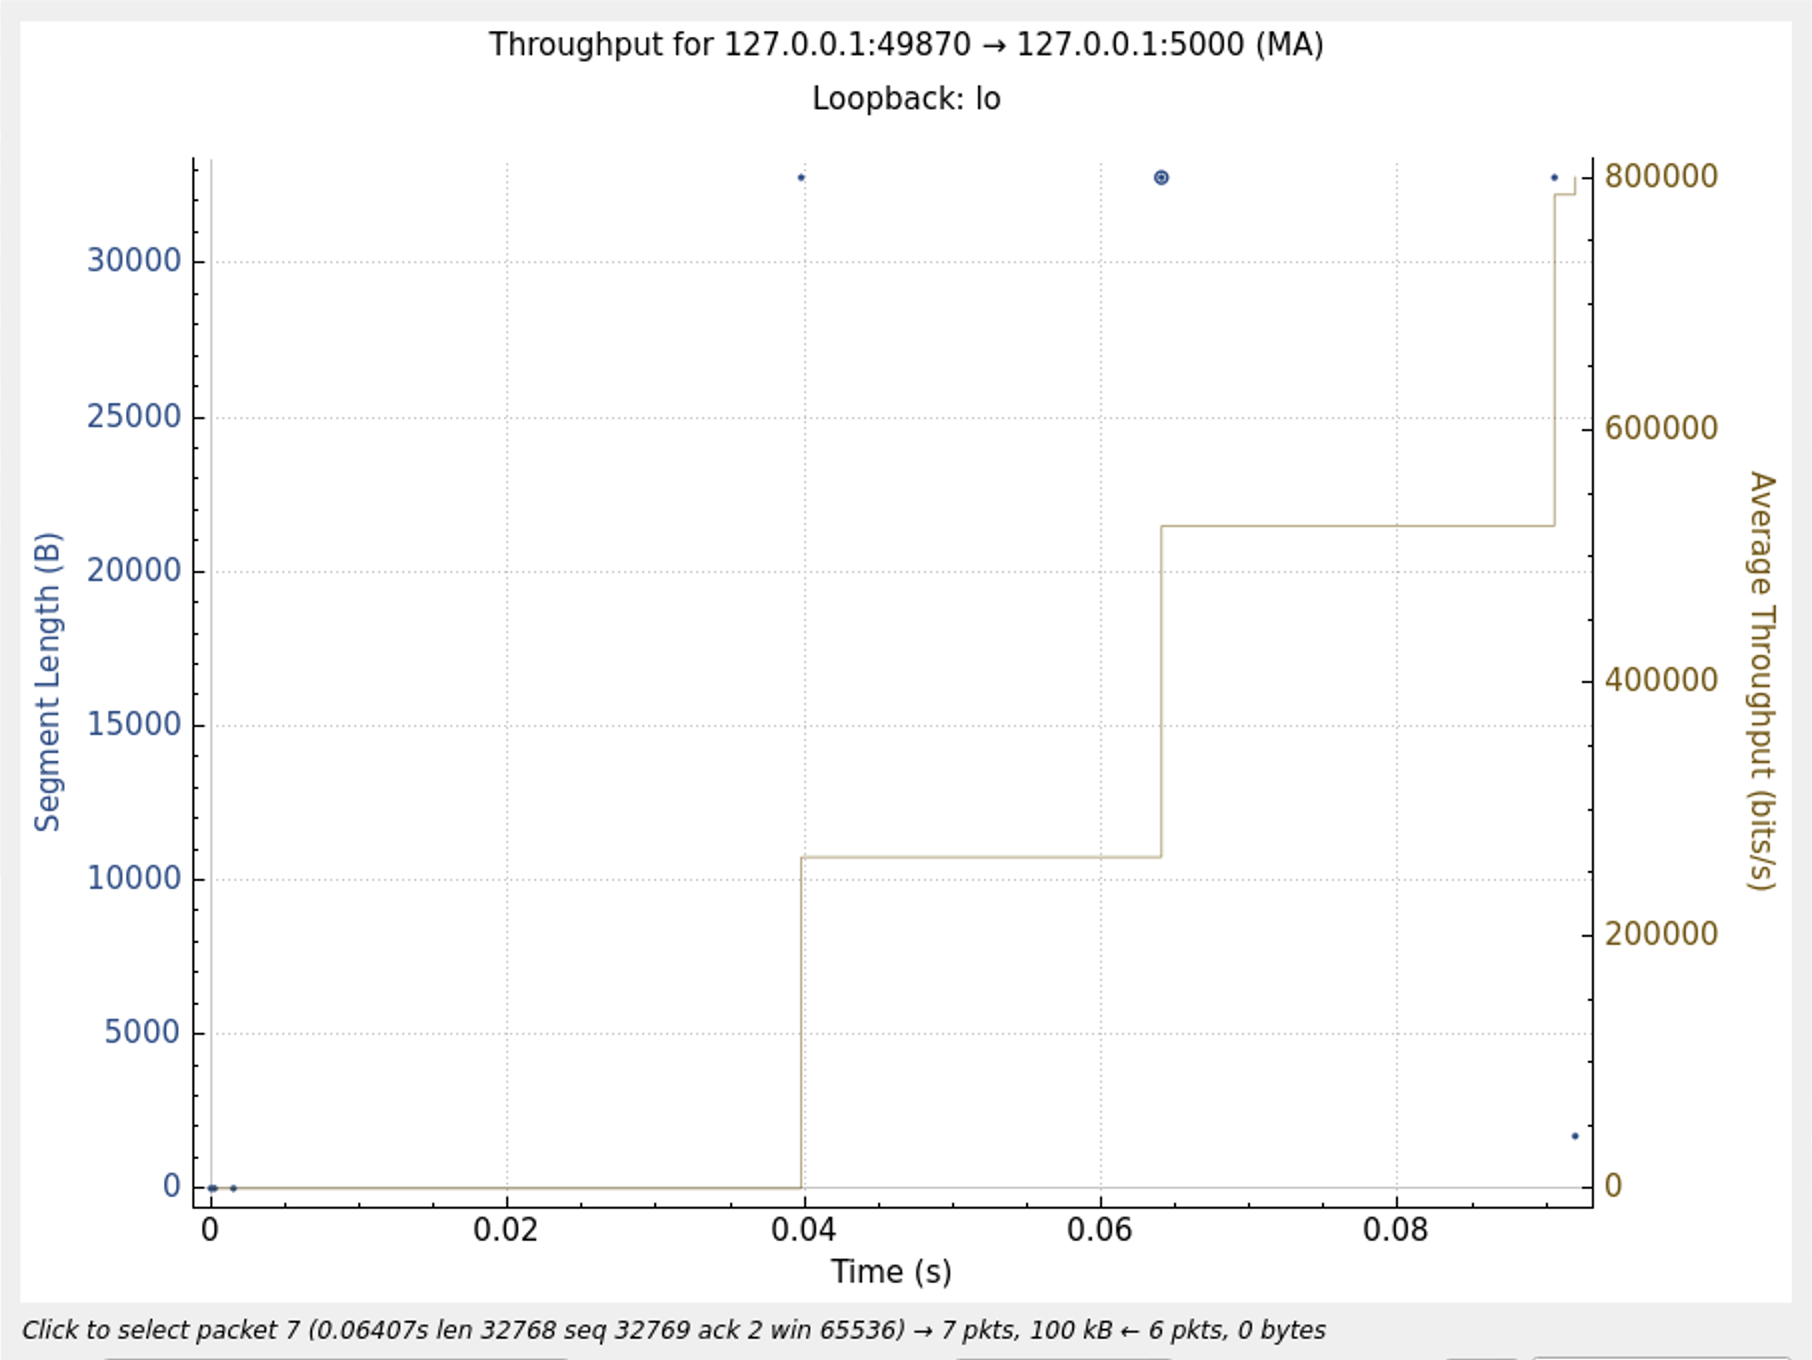
\includegraphics[width=\textwidth]{Pics/Cubic/r10mbit_s100k_th}
        \caption{10 mbit rate}
    \end{subfigure}
    \hfill
    \begin{subfigure}[b]{0.45\textwidth}
        \centering
        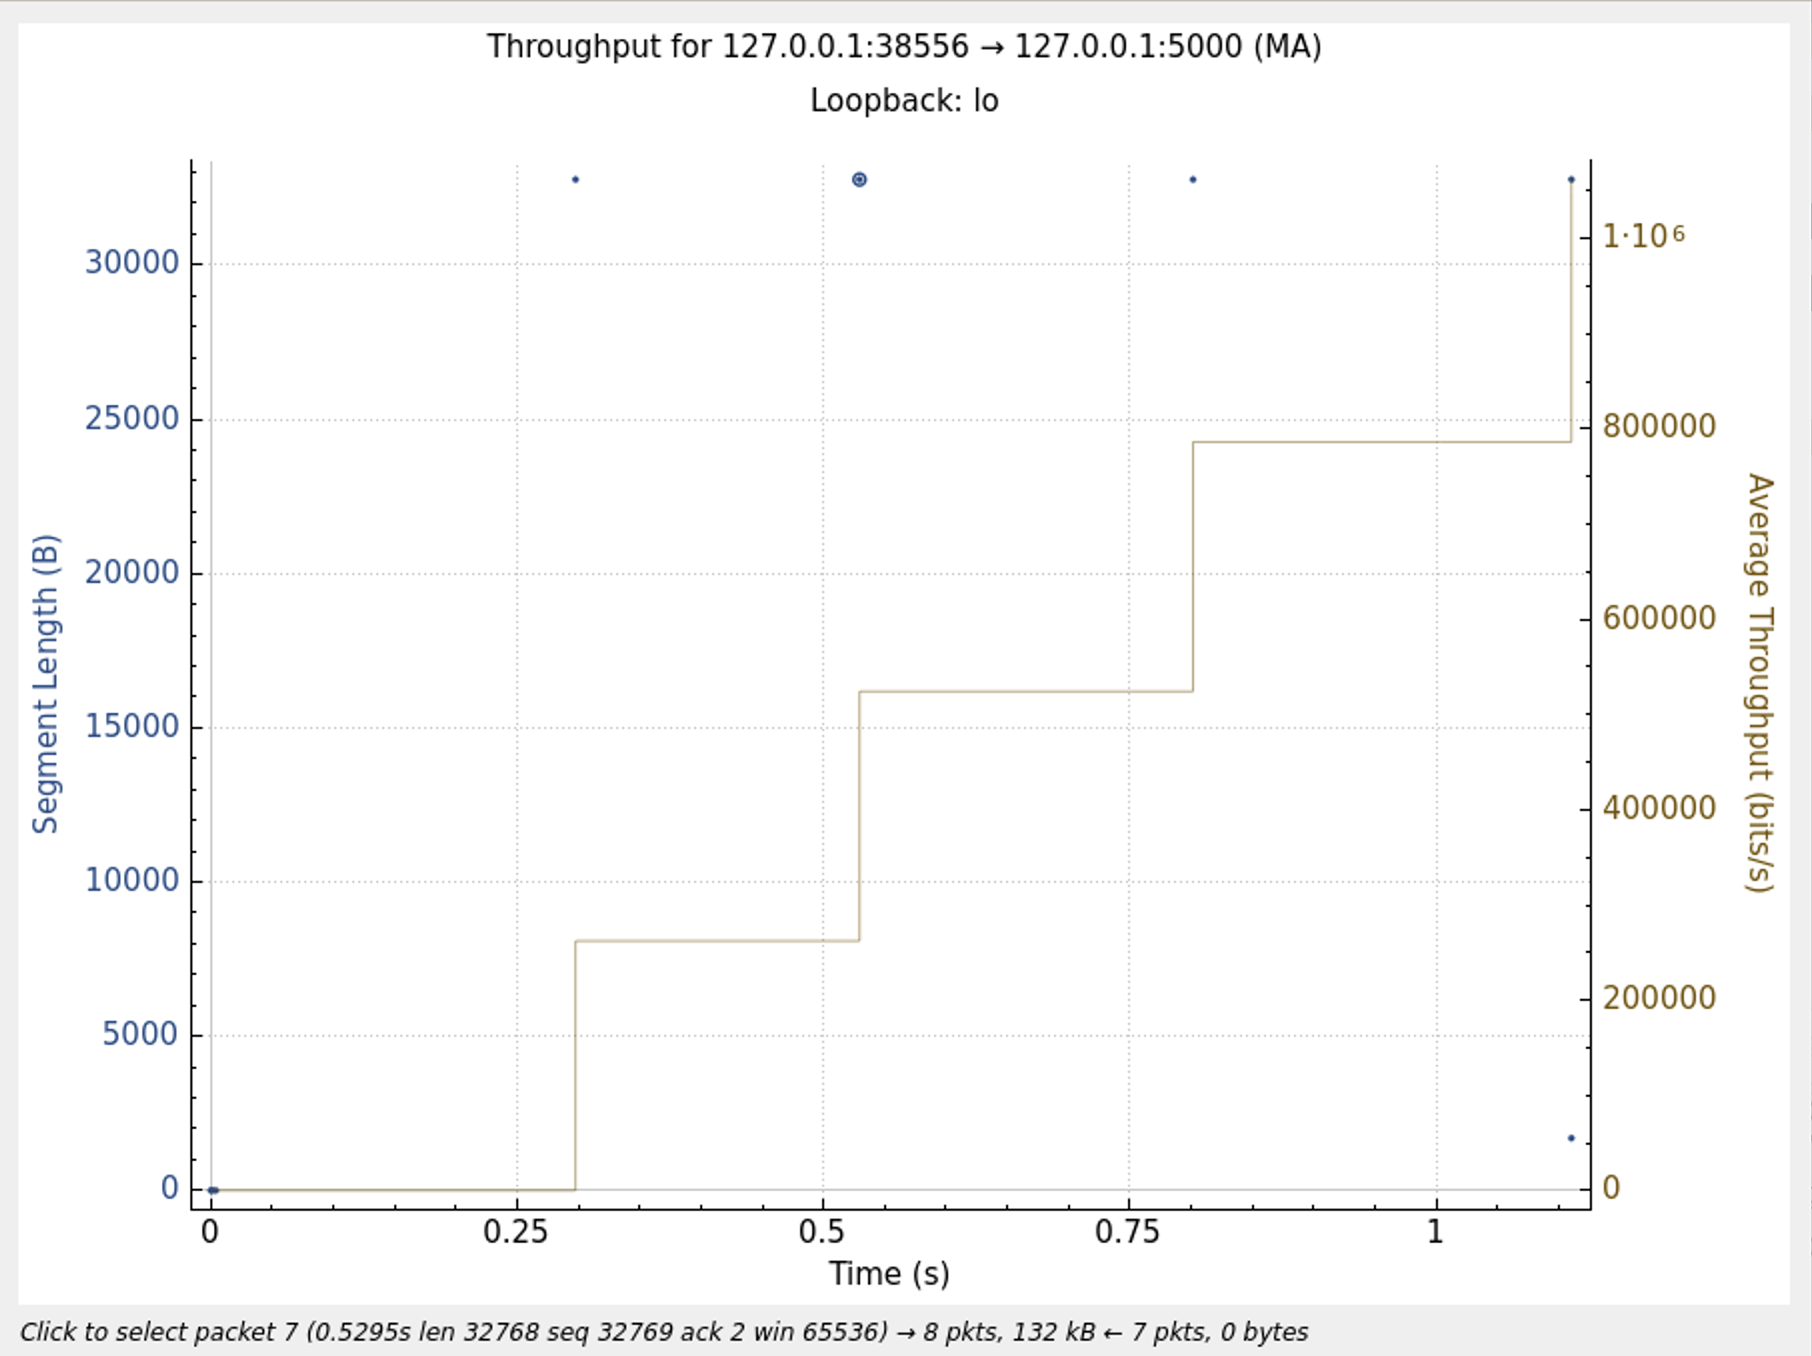
\includegraphics[width=\textwidth]{Pics/Cubic/r1mbit_s100k_th}
        \caption{1 mbit rate}
    \end{subfigure}
    \medskip

    \begin{subfigure}[b]{0.45\textwidth}
        \centering
        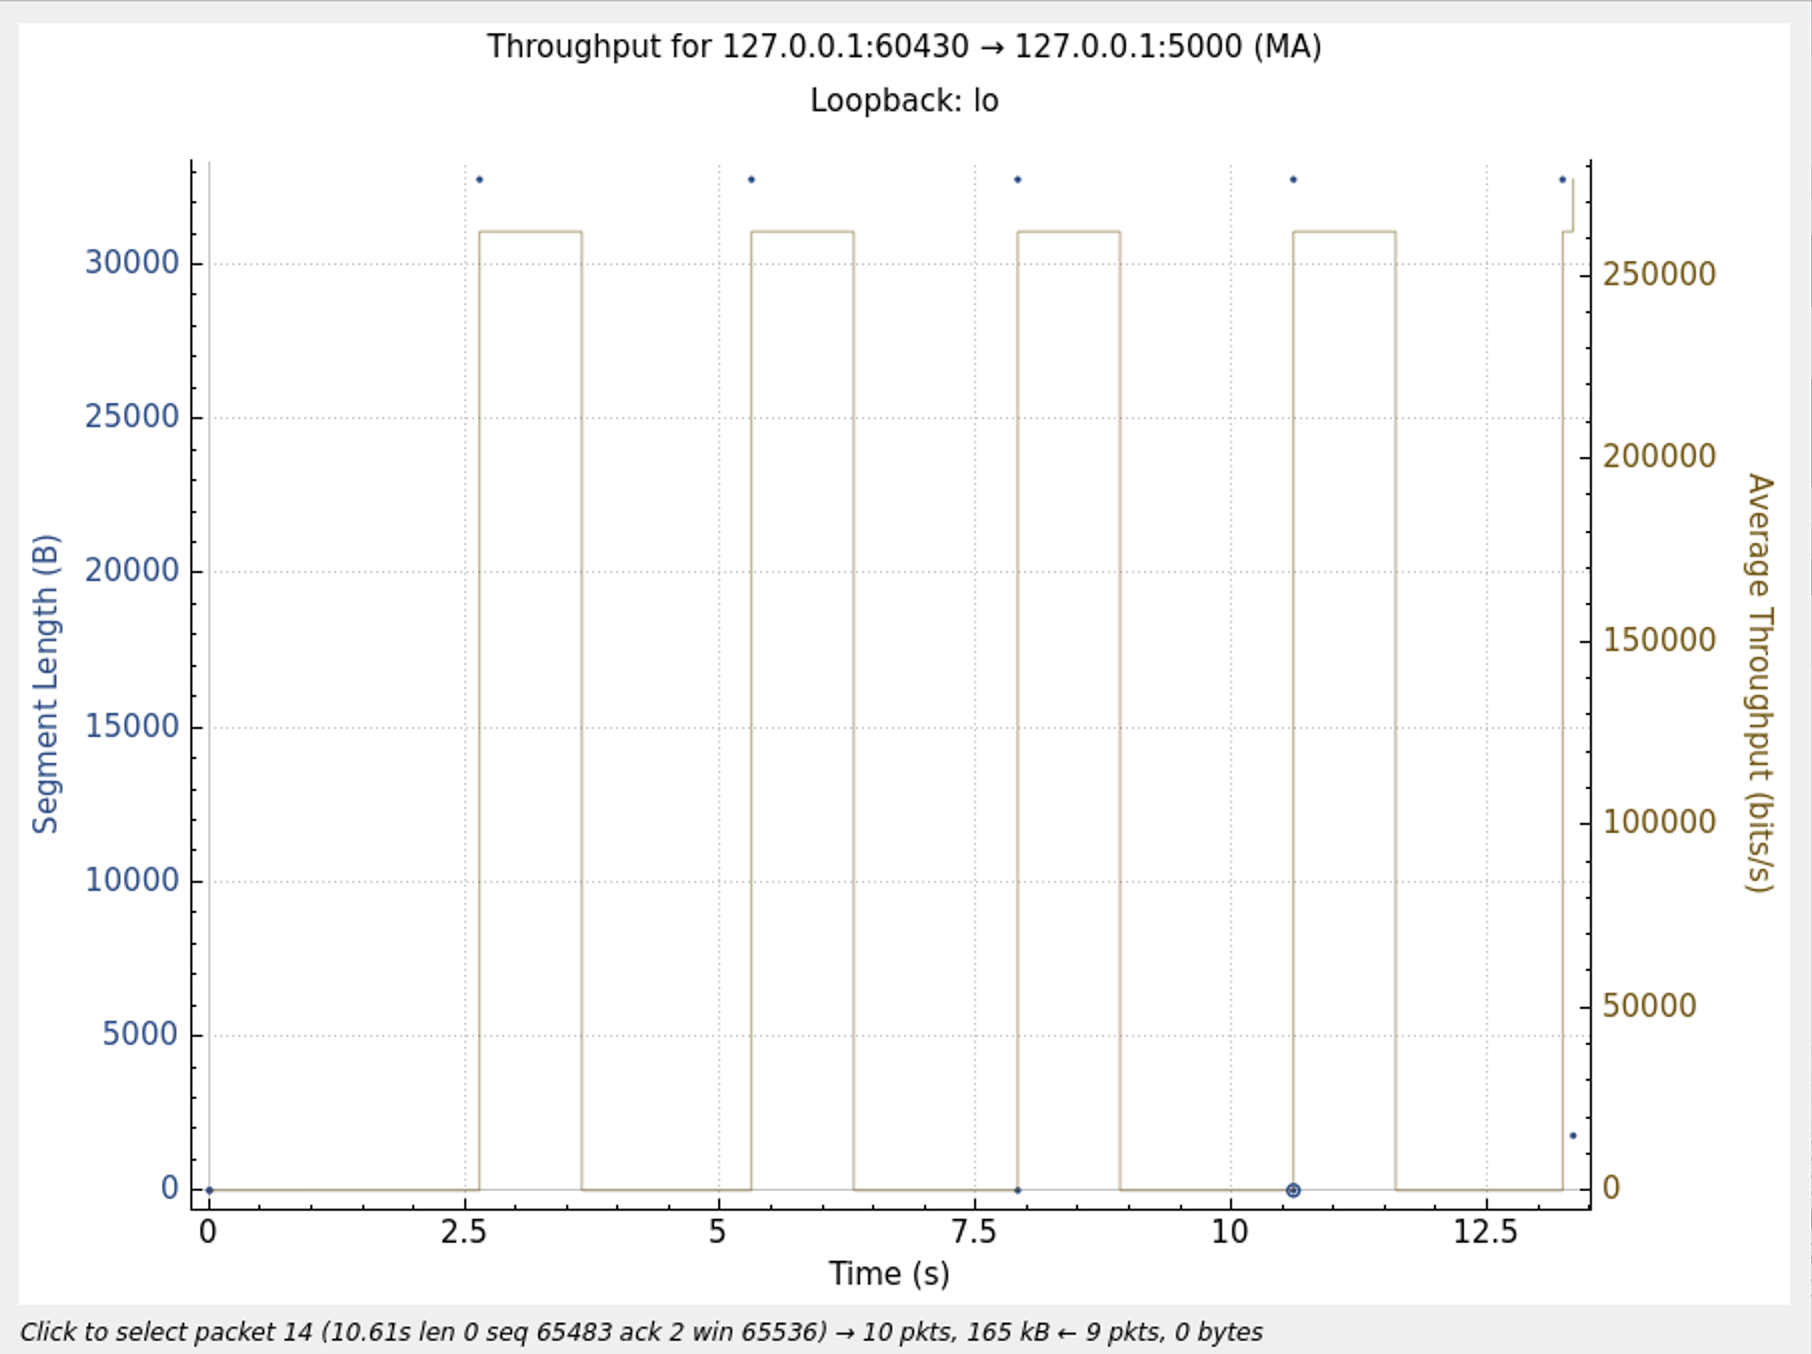
\includegraphics[width=\textwidth]{Pics/Cubic/r100kbit_s100k_th}
        \caption{100 kbit rate}
    \end{subfigure}
    \hfill
    \begin{subfigure}[b]{0.45\textwidth}
        \centering
        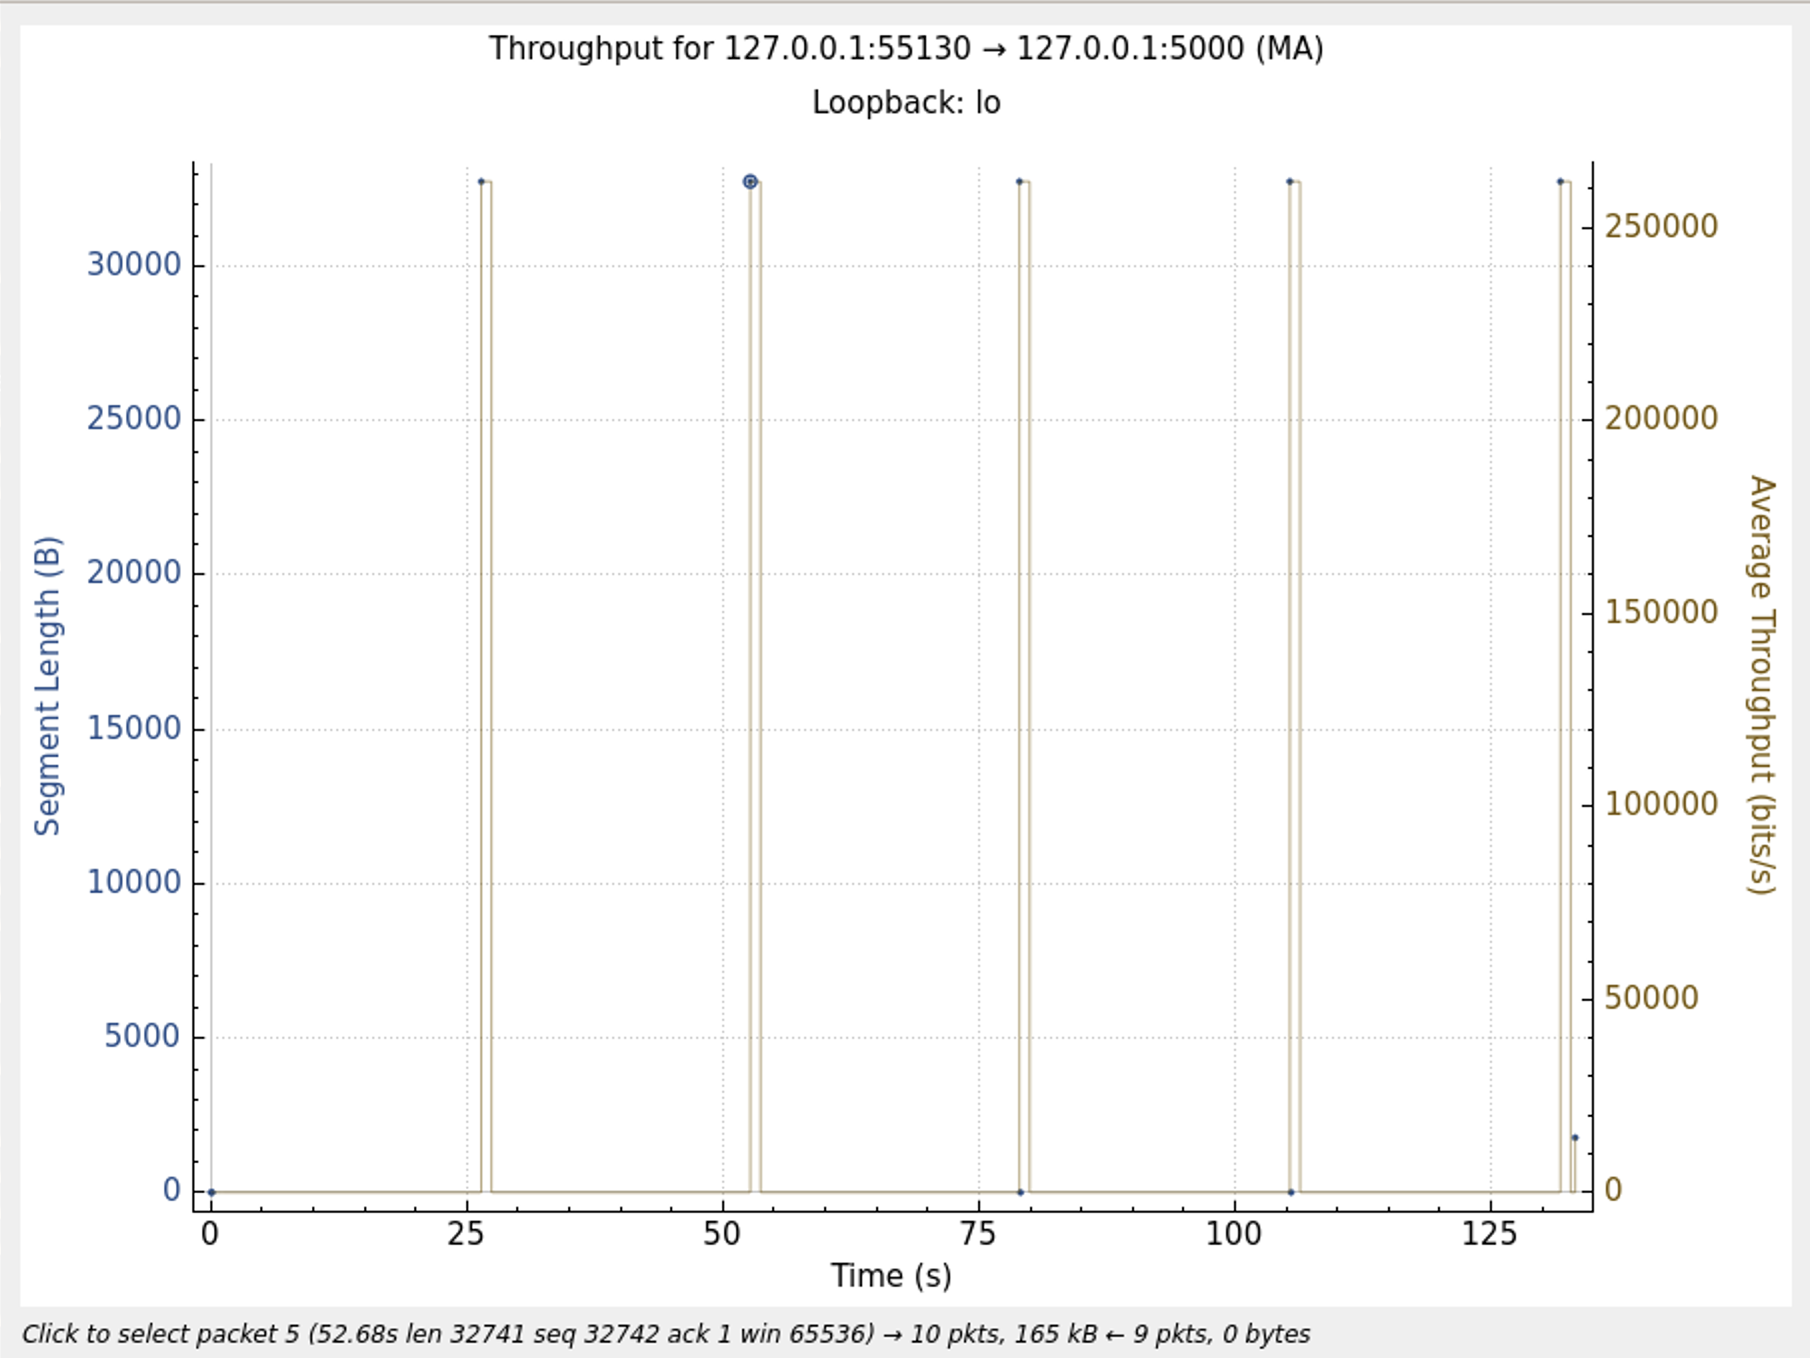
\includegraphics[width=\textwidth]{Pics/Cubic/r10kbit_s100kbit_th}
        \caption{10 kbit rate}
    \end{subfigure}
    \caption{Comparison of the throughput for 100kbit of data sent with different rate limits.}
    \label{fig:four_images}
\end{figure}

Finally with a transfer data size of 1mb we get the following.
\begin{figure}[H]
    \centering
    \begin{subfigure}[b]{0.45\textwidth}
        \centering
        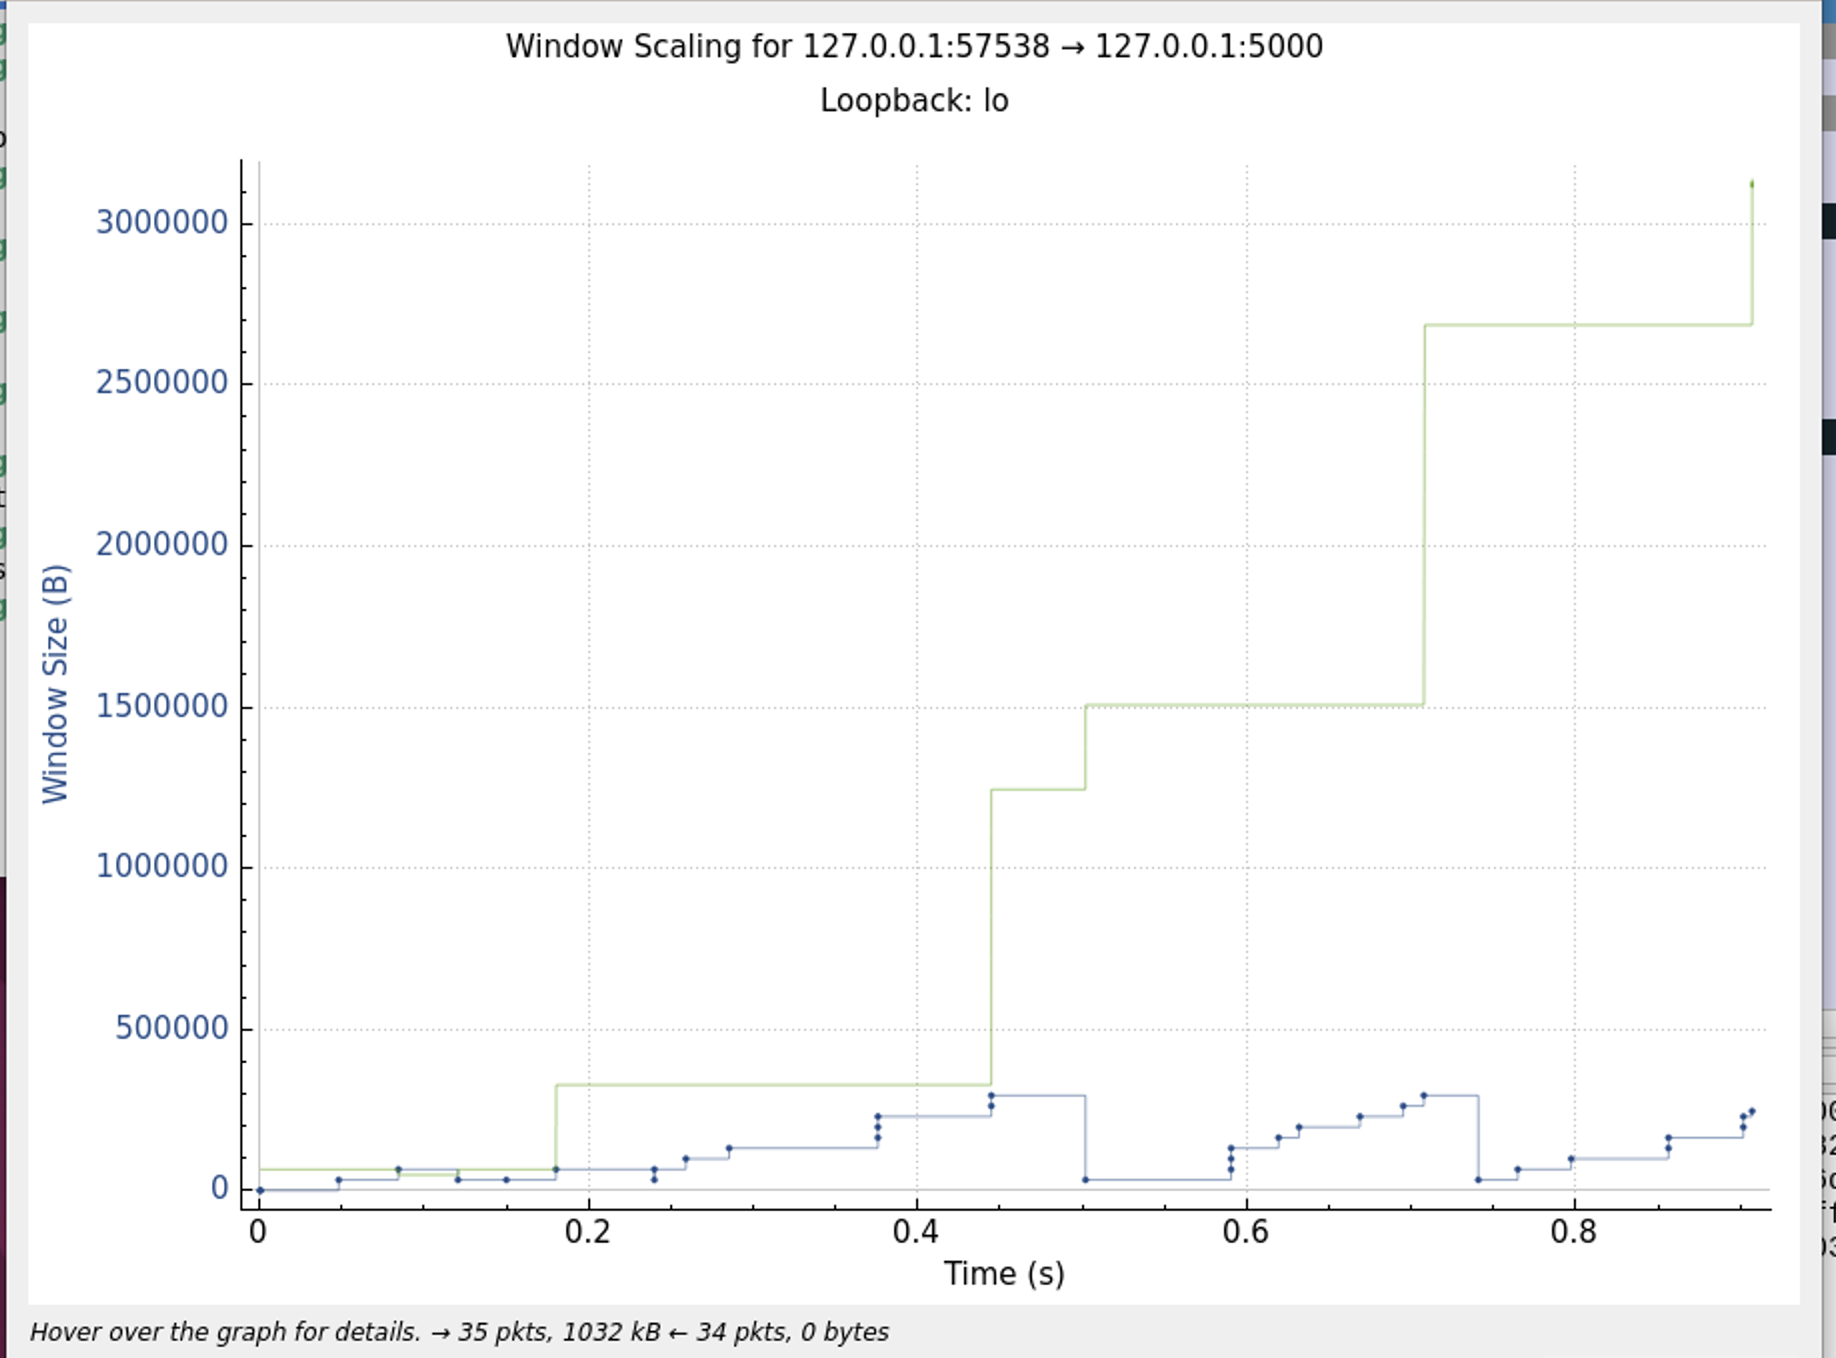
\includegraphics[width=\textwidth]{Pics/Cubic/r10mbit_s1m_ws}
        \caption{10 mbit rate }
    \end{subfigure}
    \hfill
    \begin{subfigure}[b]{0.45\textwidth}
        \centering
        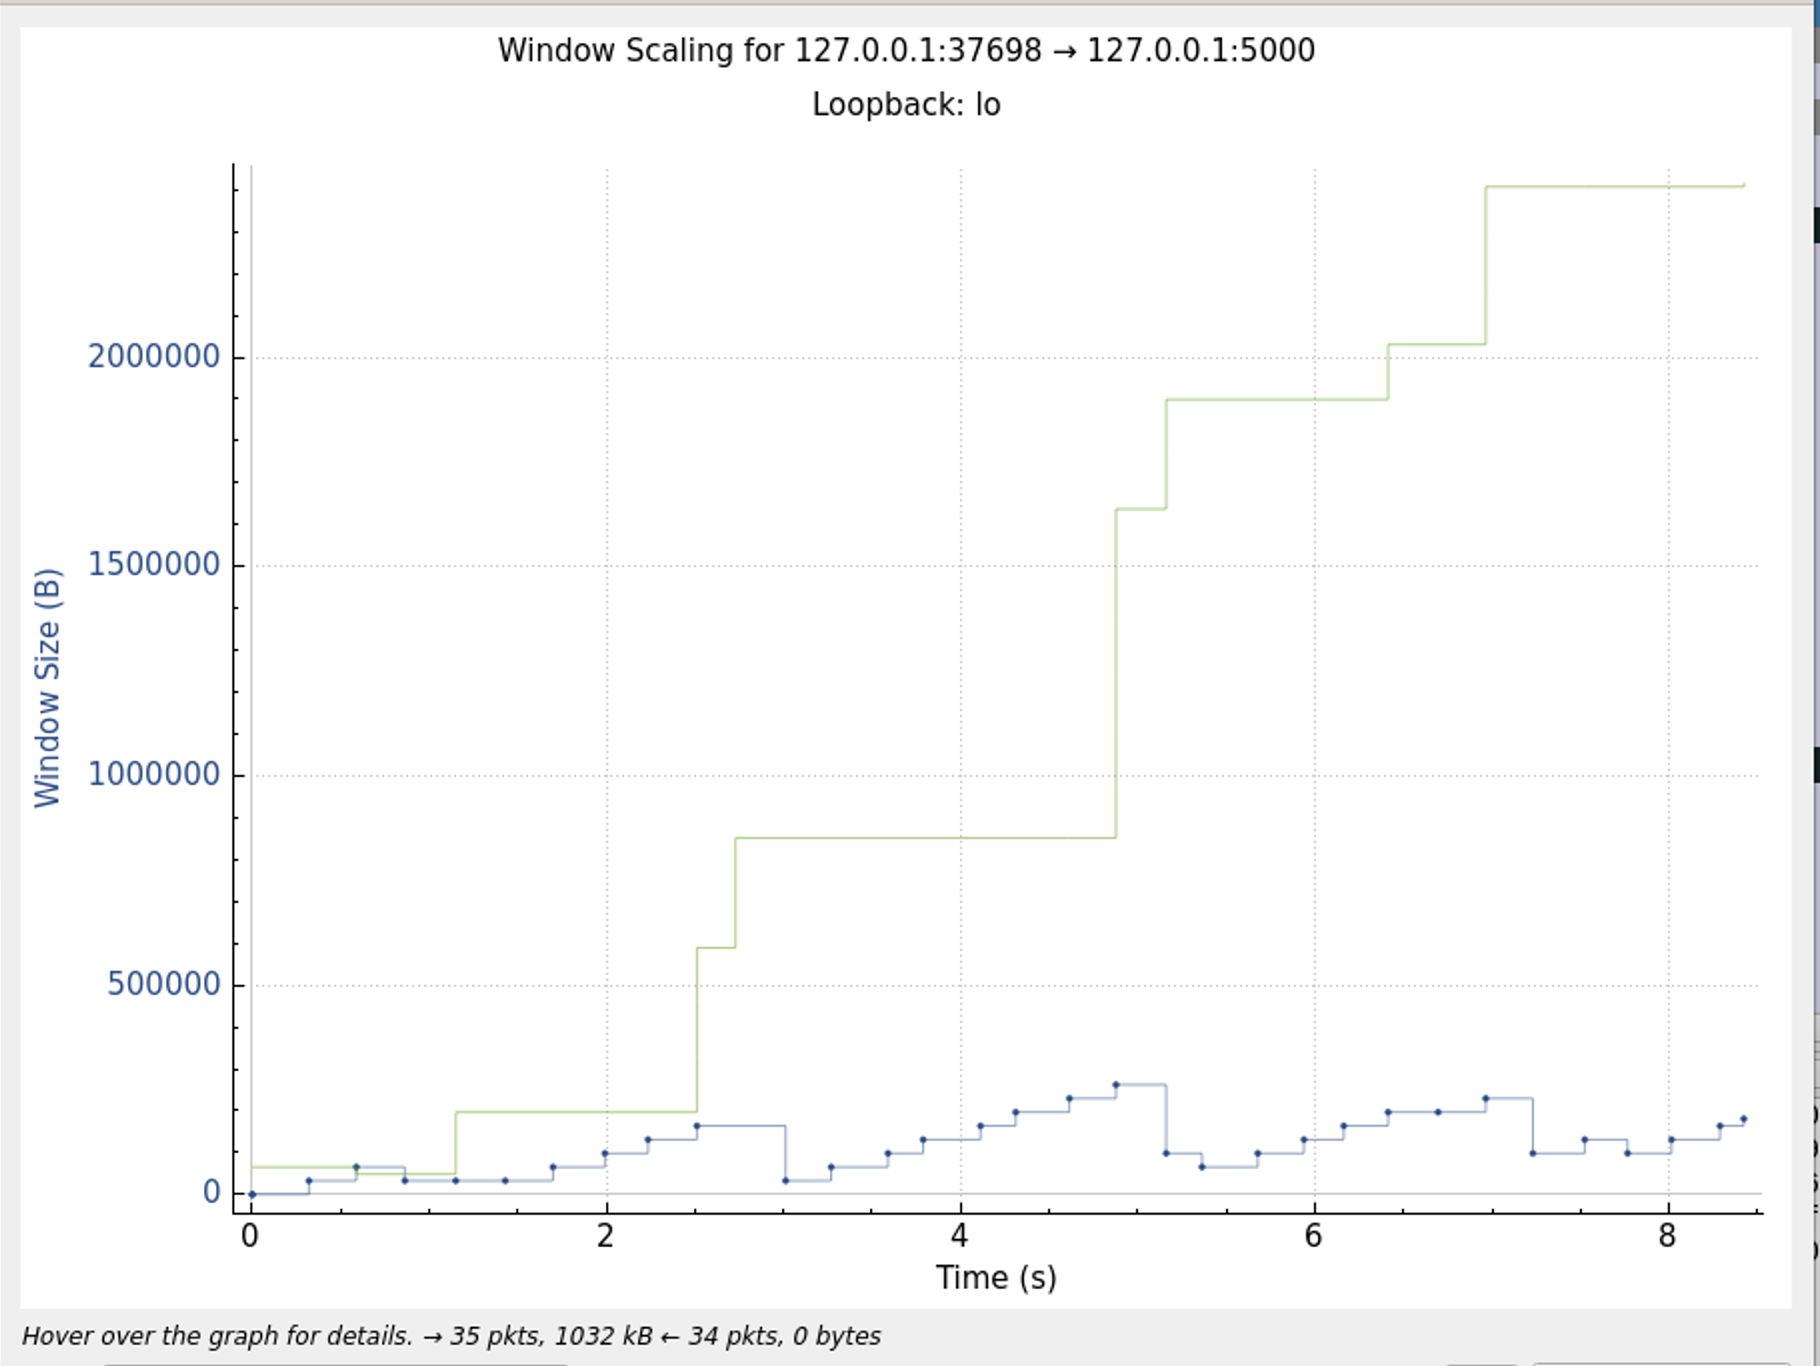
\includegraphics[width=\textwidth]{Pics/Cubic/r1mbit_s1m_ws}
        \caption{1 mbit rate}
    \end{subfigure}
    \medskip

    \begin{subfigure}[b]{0.45\textwidth}
        \centering
        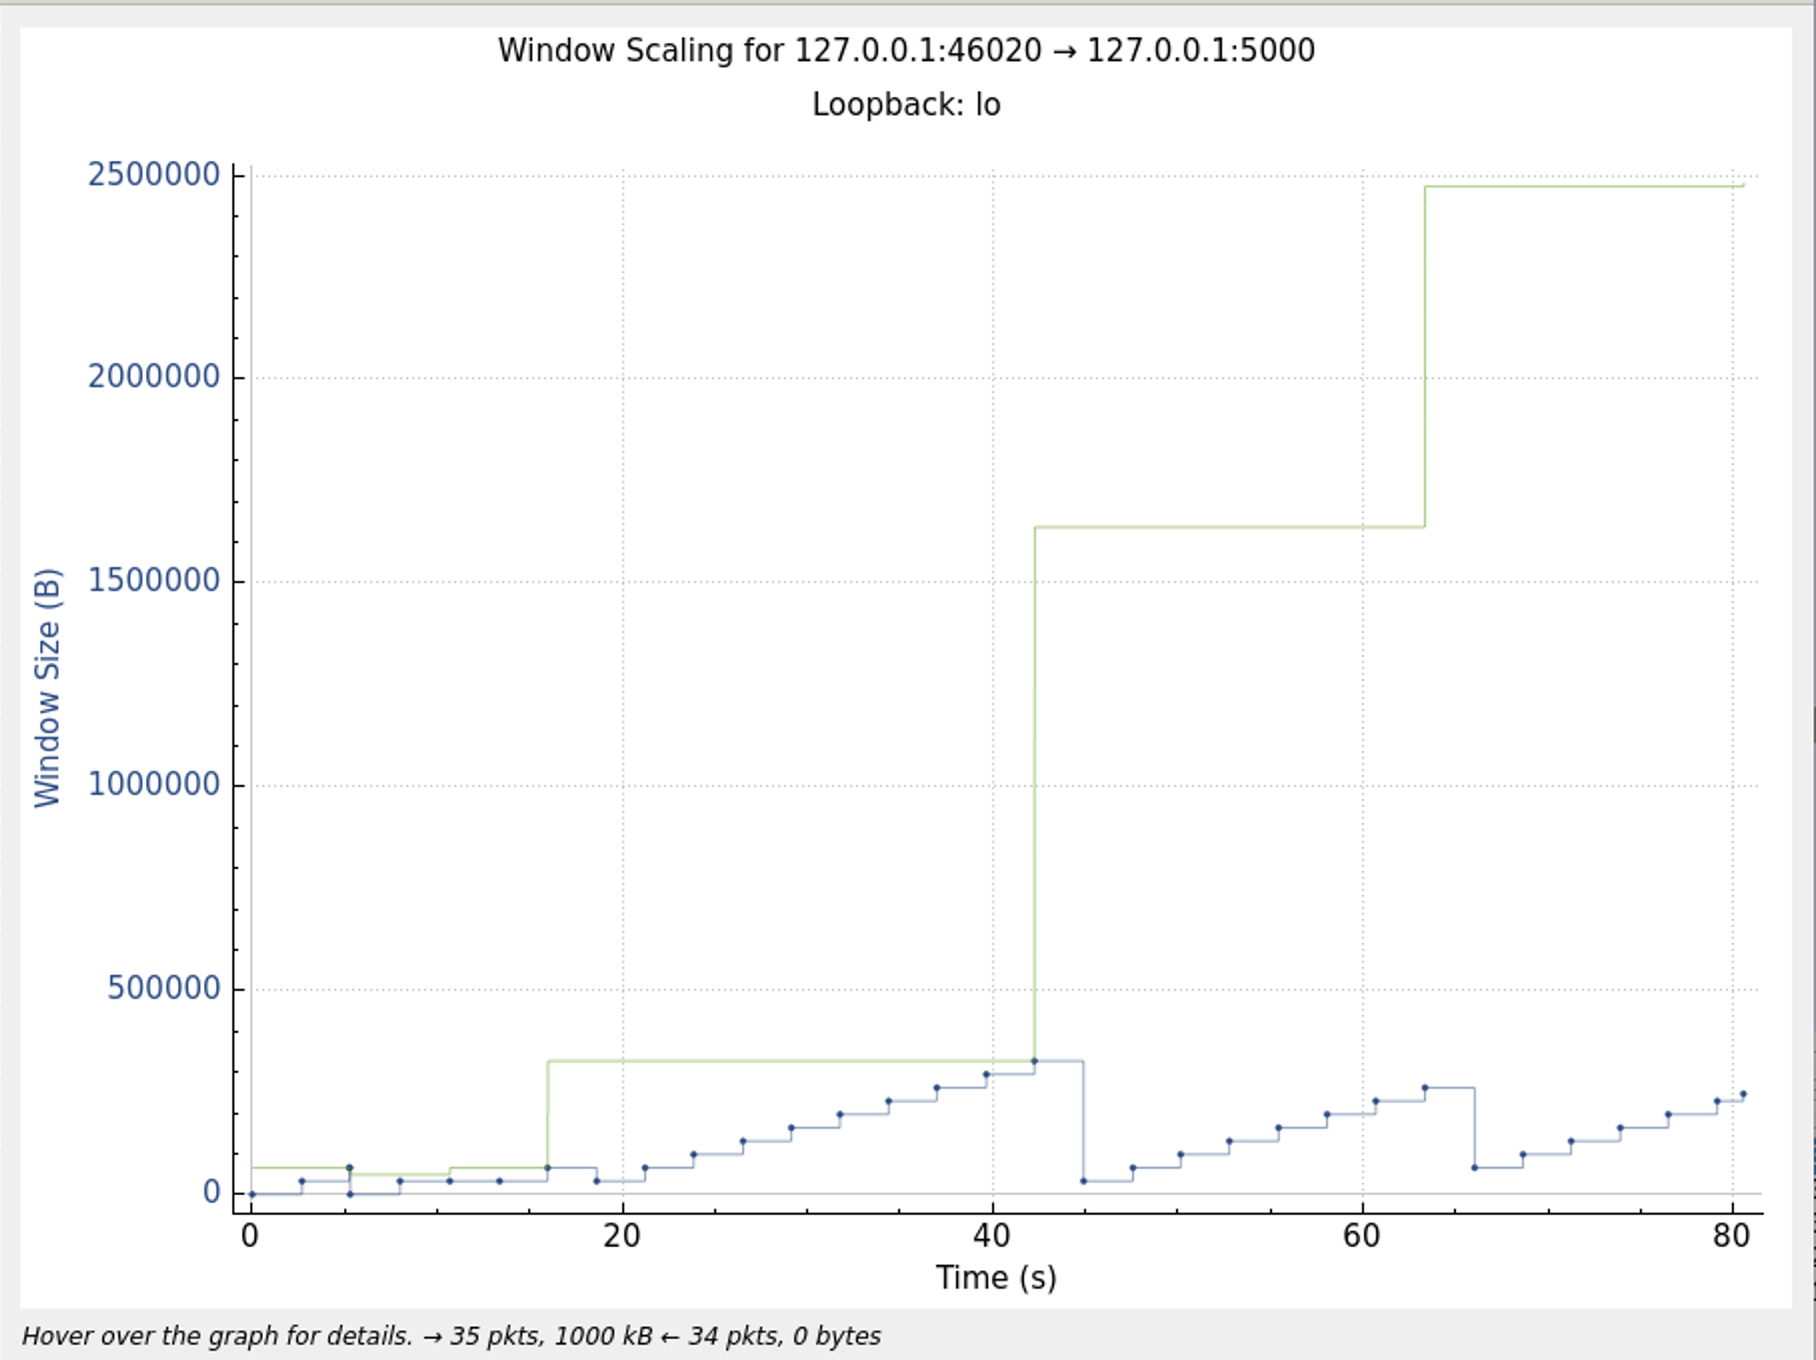
\includegraphics[width=\textwidth]{Pics/Cubic/r100kbit_s1m_ws}
        \caption{100 kbit rate}
    \end{subfigure}
    \hfill
    \begin{subfigure}[b]{0.45\textwidth}
        \centering
        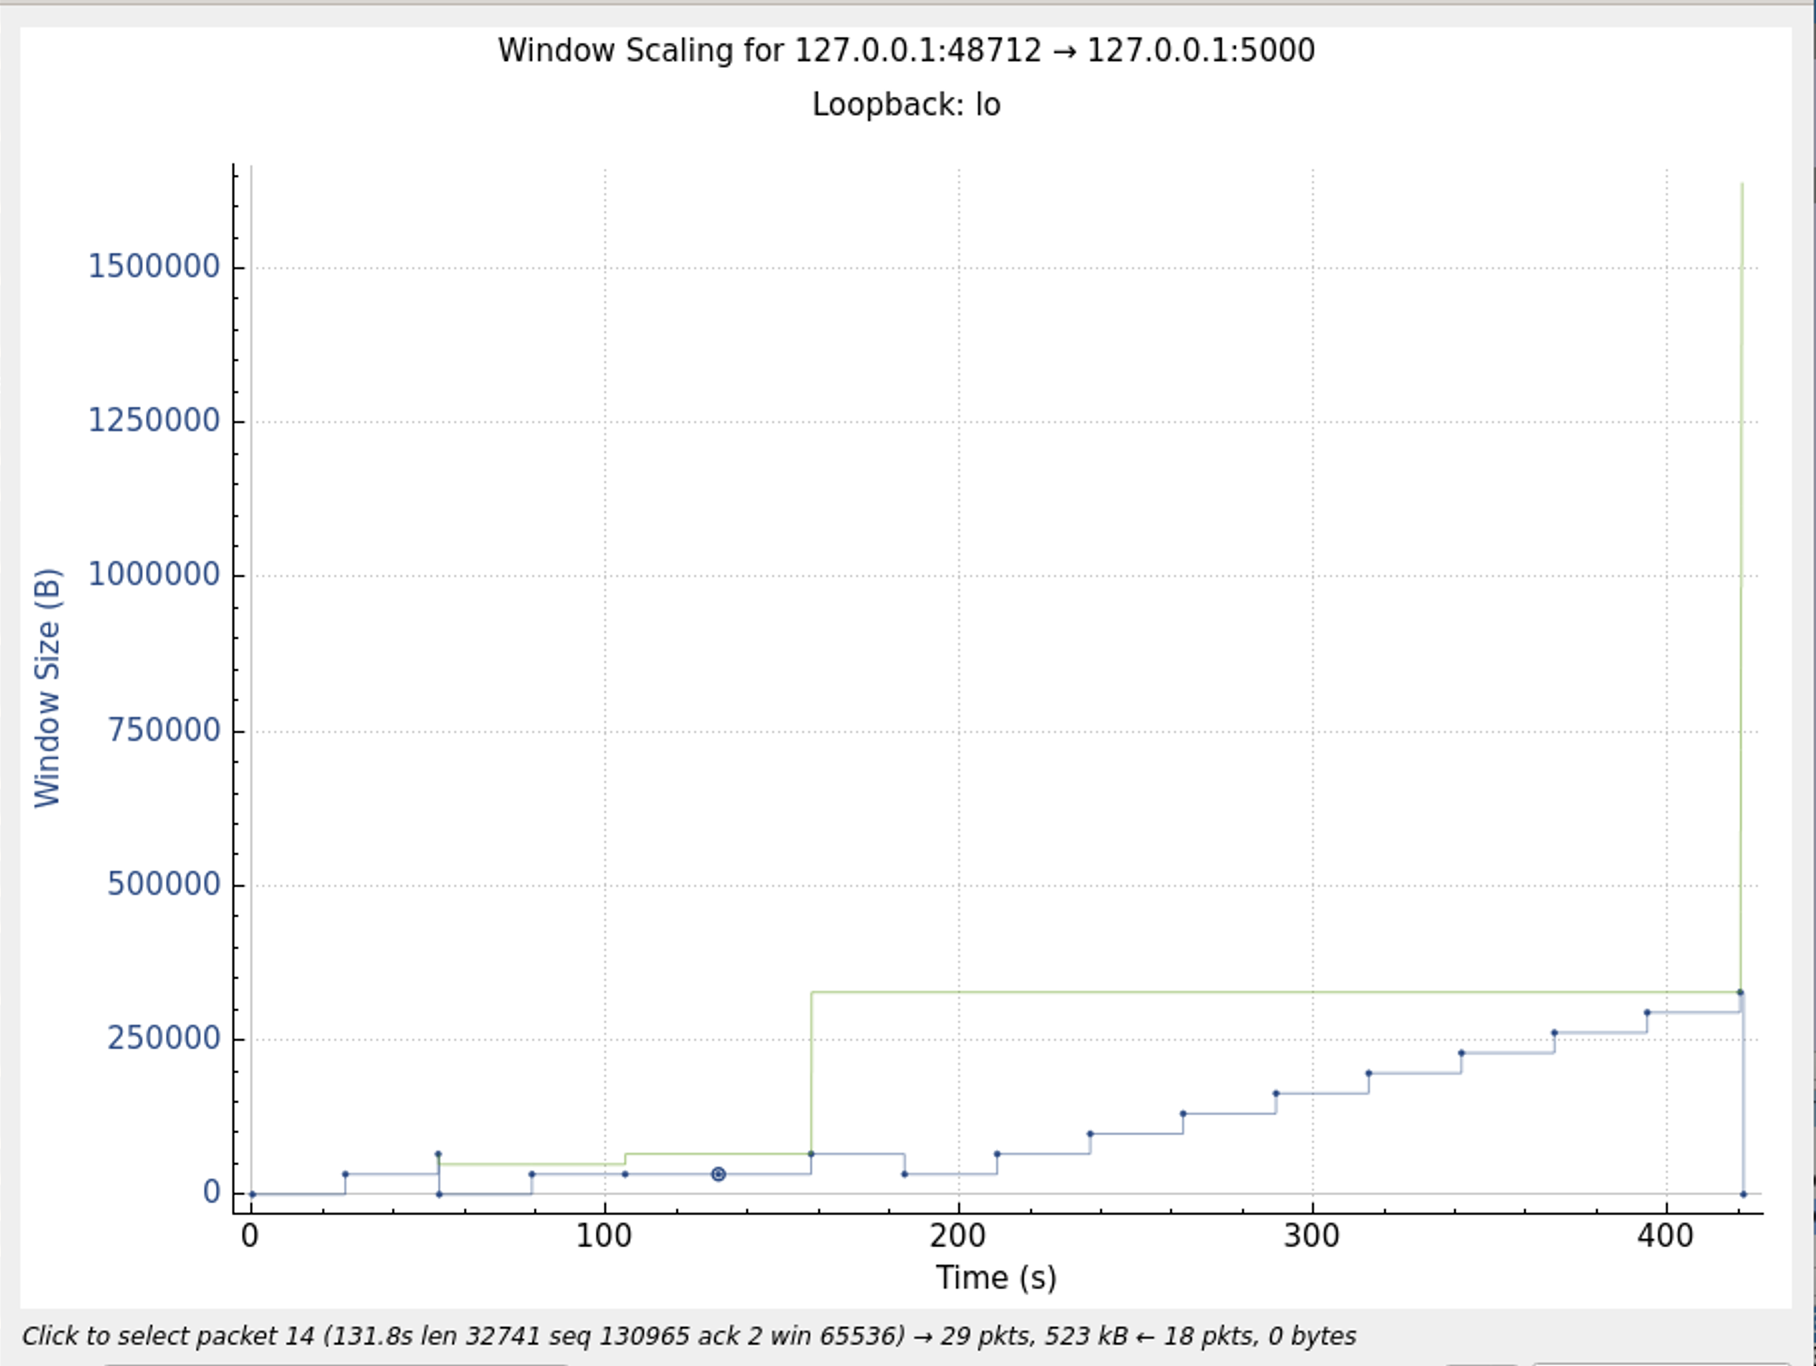
\includegraphics[width=\textwidth]{Pics/Cubic/r10kbit_s1m_ws}
        \caption{10 kbit rate. BORKED}
    \end{subfigure}
    \caption{Comparison of the window scaling for 1mbit of data sent with different rate limits.}
    \label{fig:four_images}
\end{figure}

\begin{figure}[H]
    \centering
    \begin{subfigure}[b]{0.45\textwidth}
        \centering
        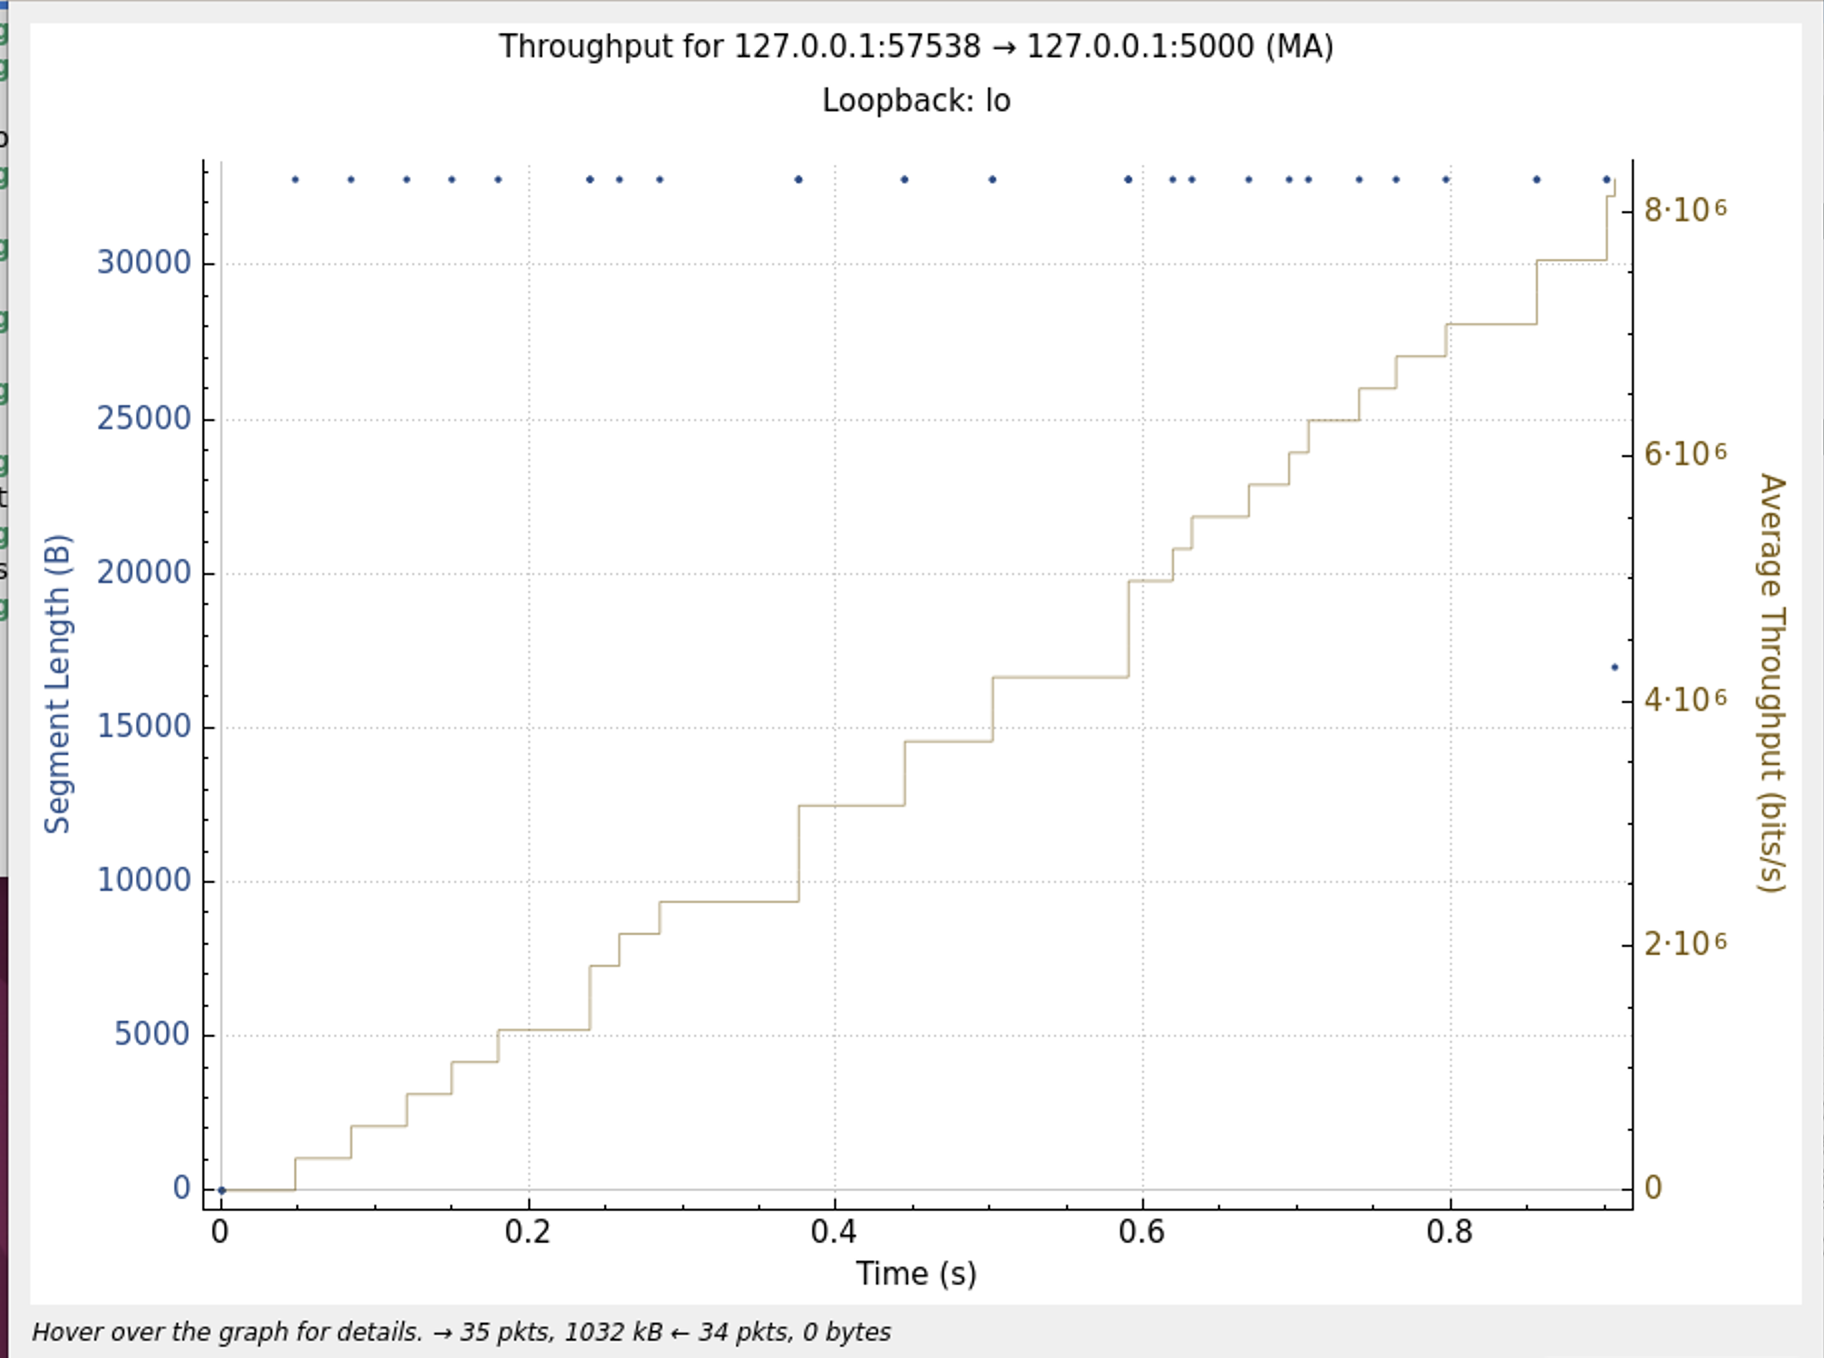
\includegraphics[width=\textwidth]{Pics/Cubic/r10mbit_s1m_th}
        \caption{10 mbit rate}
    \end{subfigure}
    \hfill
    \begin{subfigure}[b]{0.45\textwidth}
        \centering
        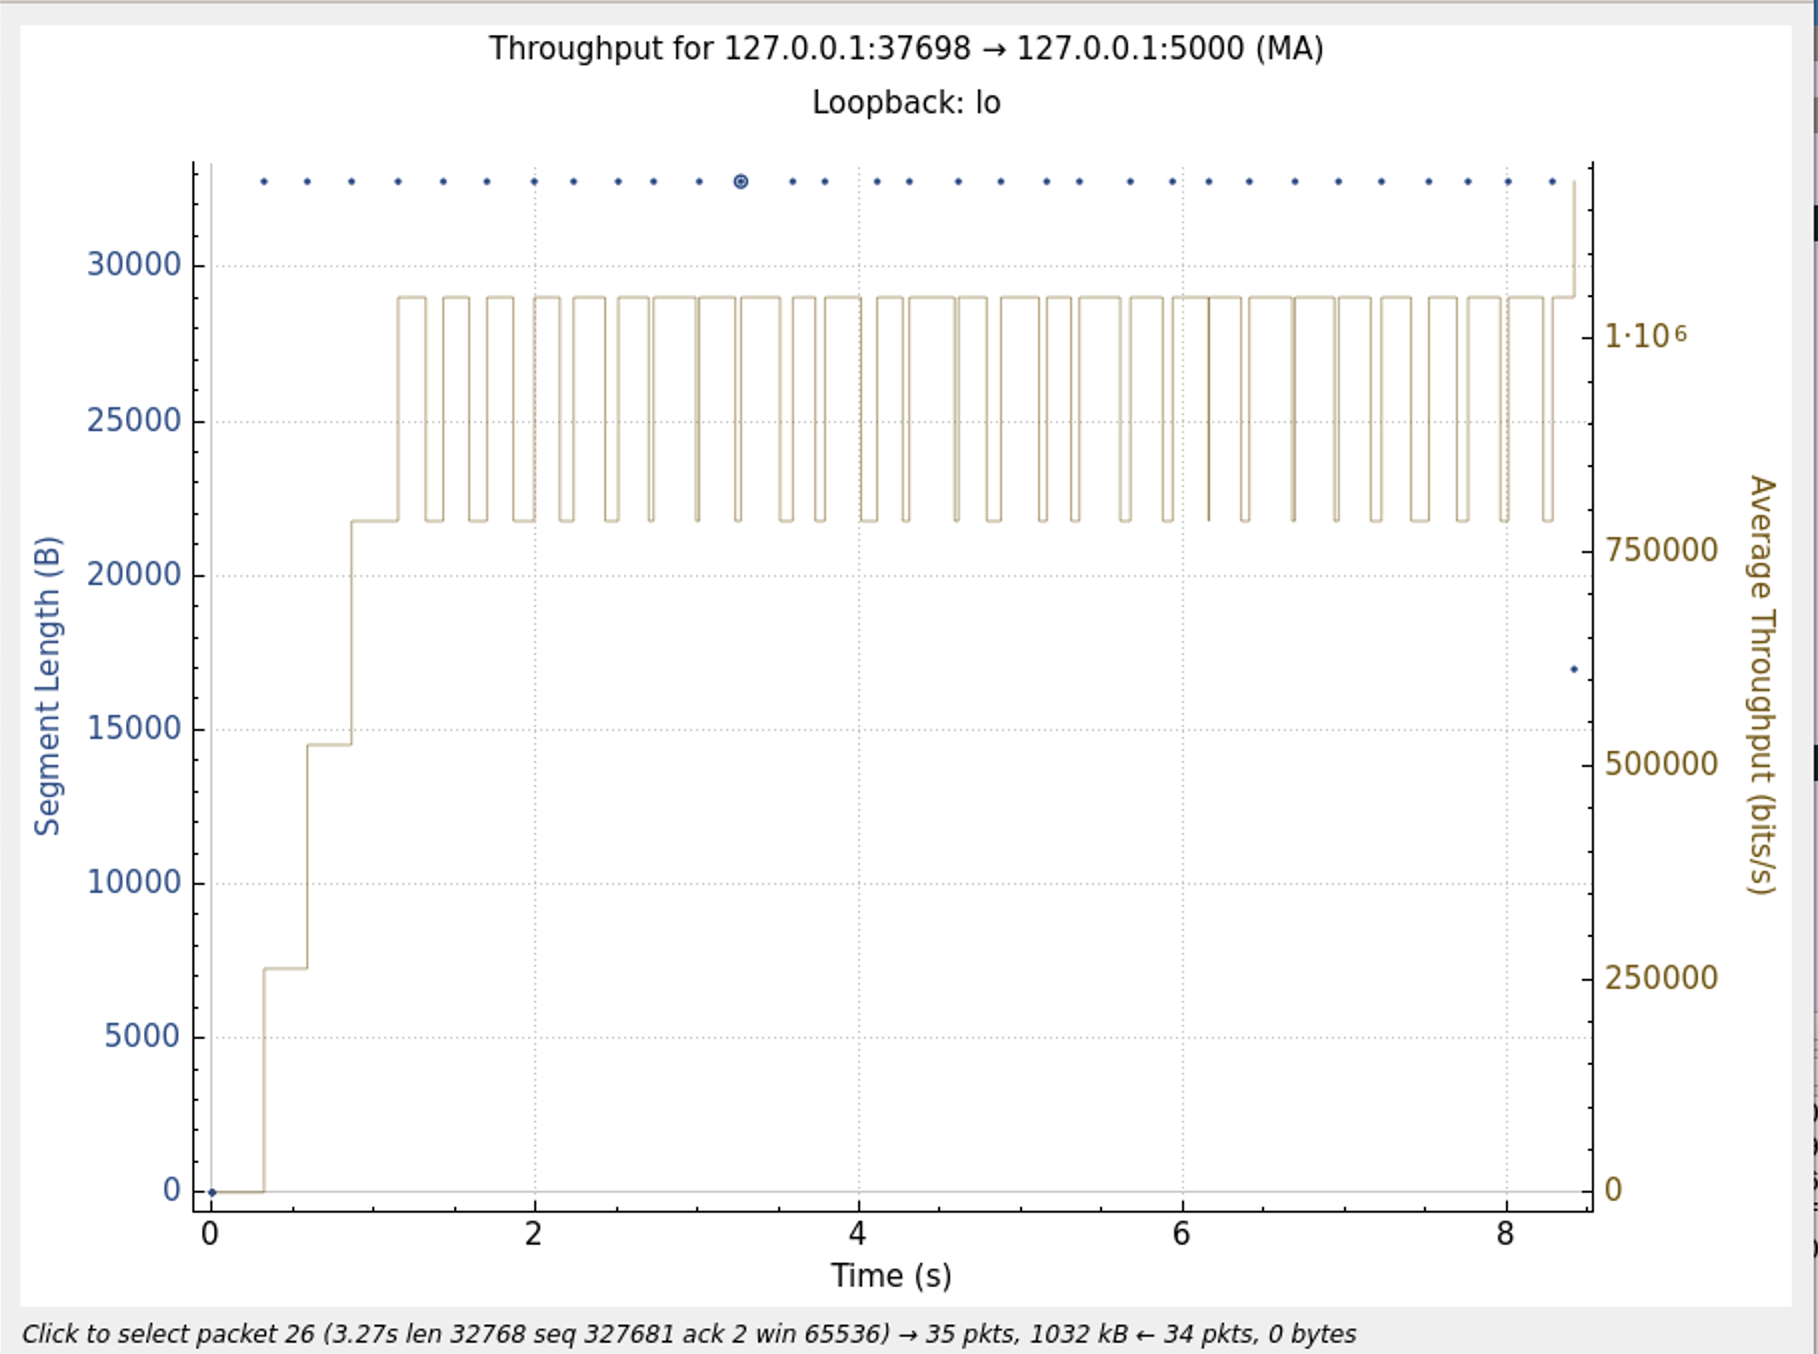
\includegraphics[width=\textwidth]{Pics/Cubic/r1mbit_s1m_th}
        \caption{1 mbit rate}
    \end{subfigure}
    \medskip

    \begin{subfigure}[b]{0.45\textwidth}
        \centering
        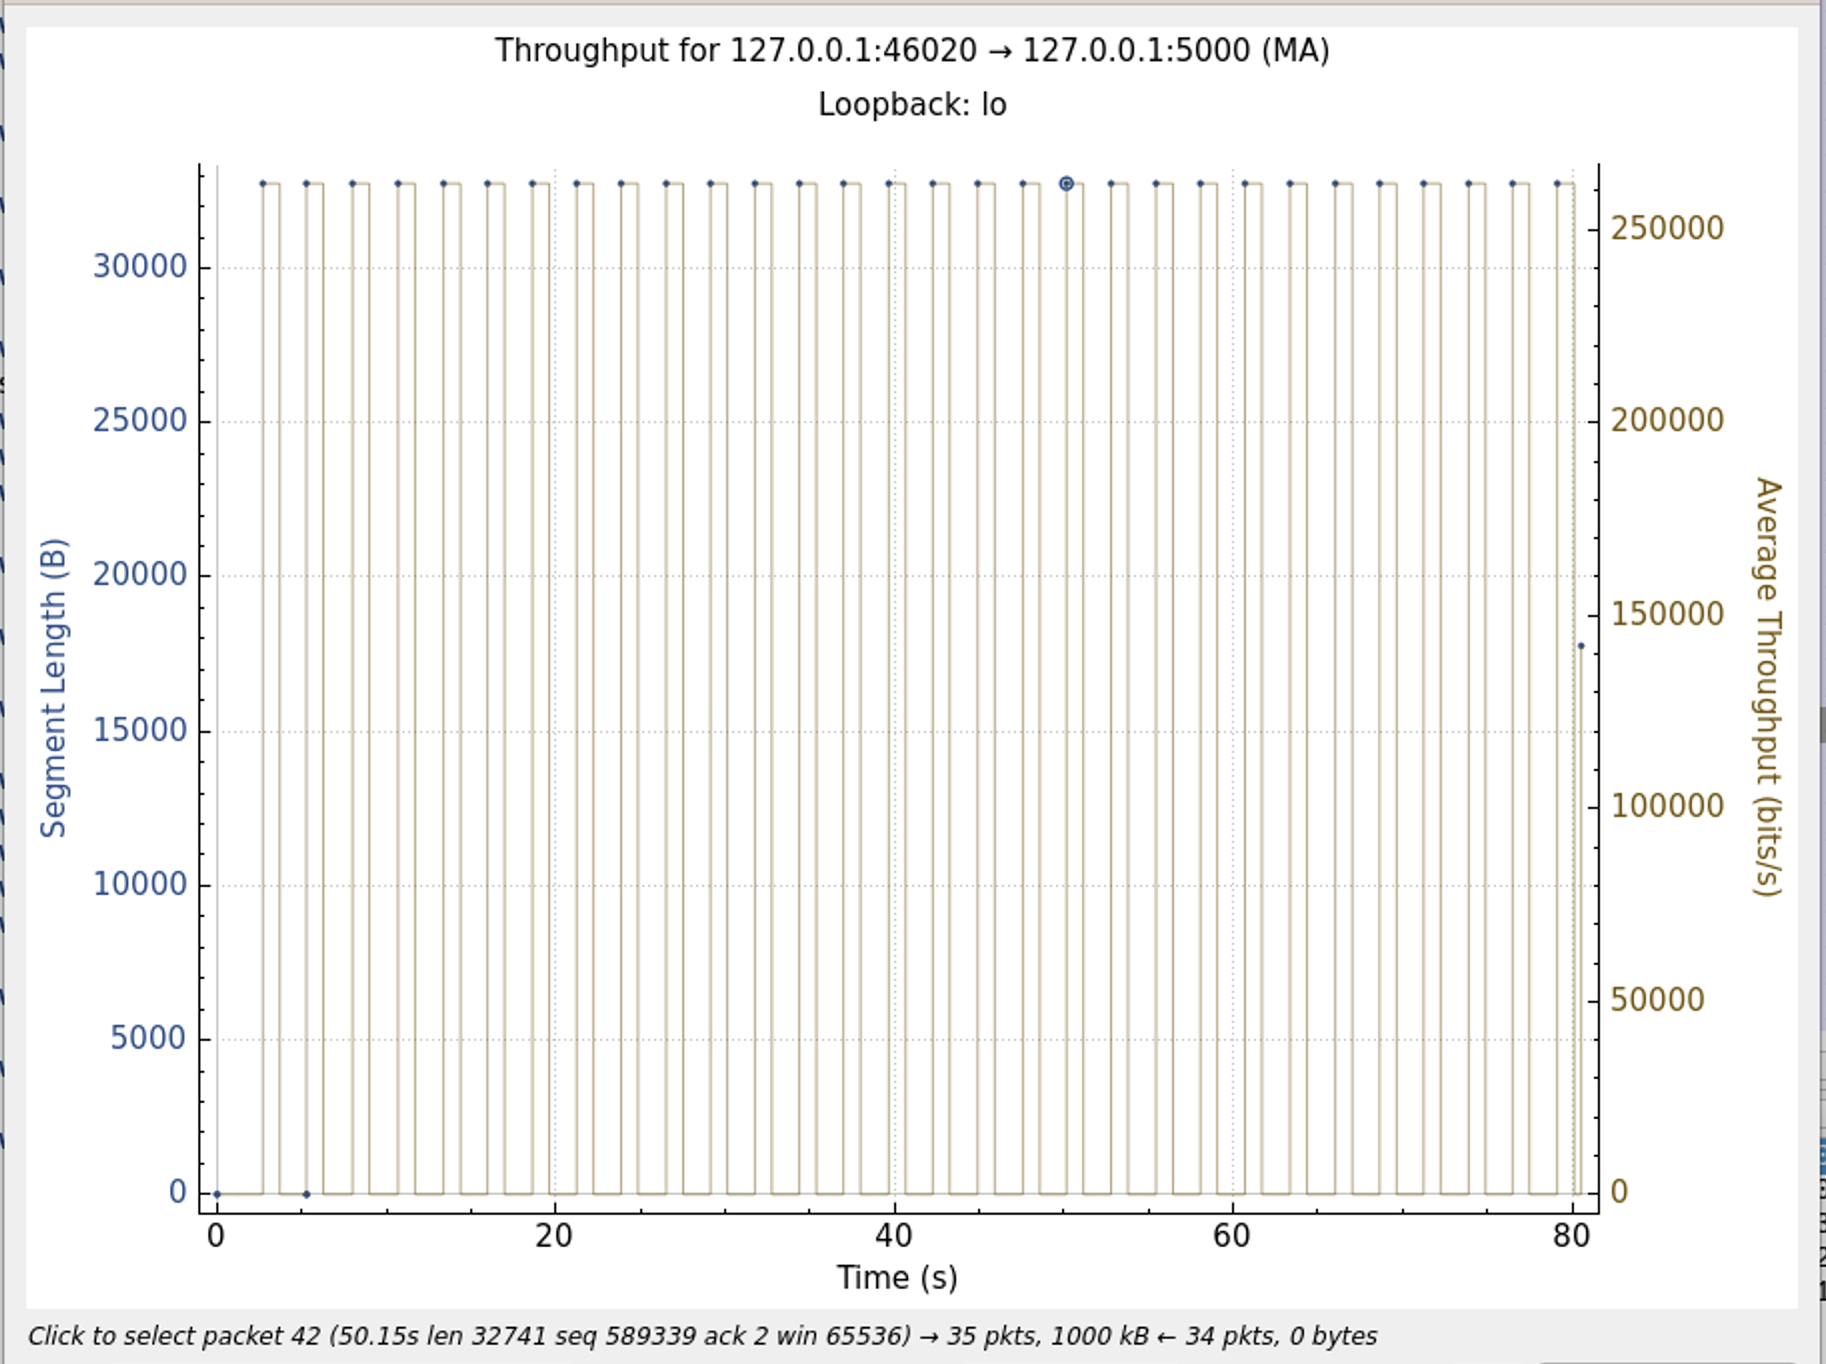
\includegraphics[width=\textwidth]{Pics/Cubic/r100kbit_s1m_th}
        \caption{100 kbit rate}
    \end{subfigure}
    \hfill
    \begin{subfigure}[b]{0.45\textwidth}
        \centering
        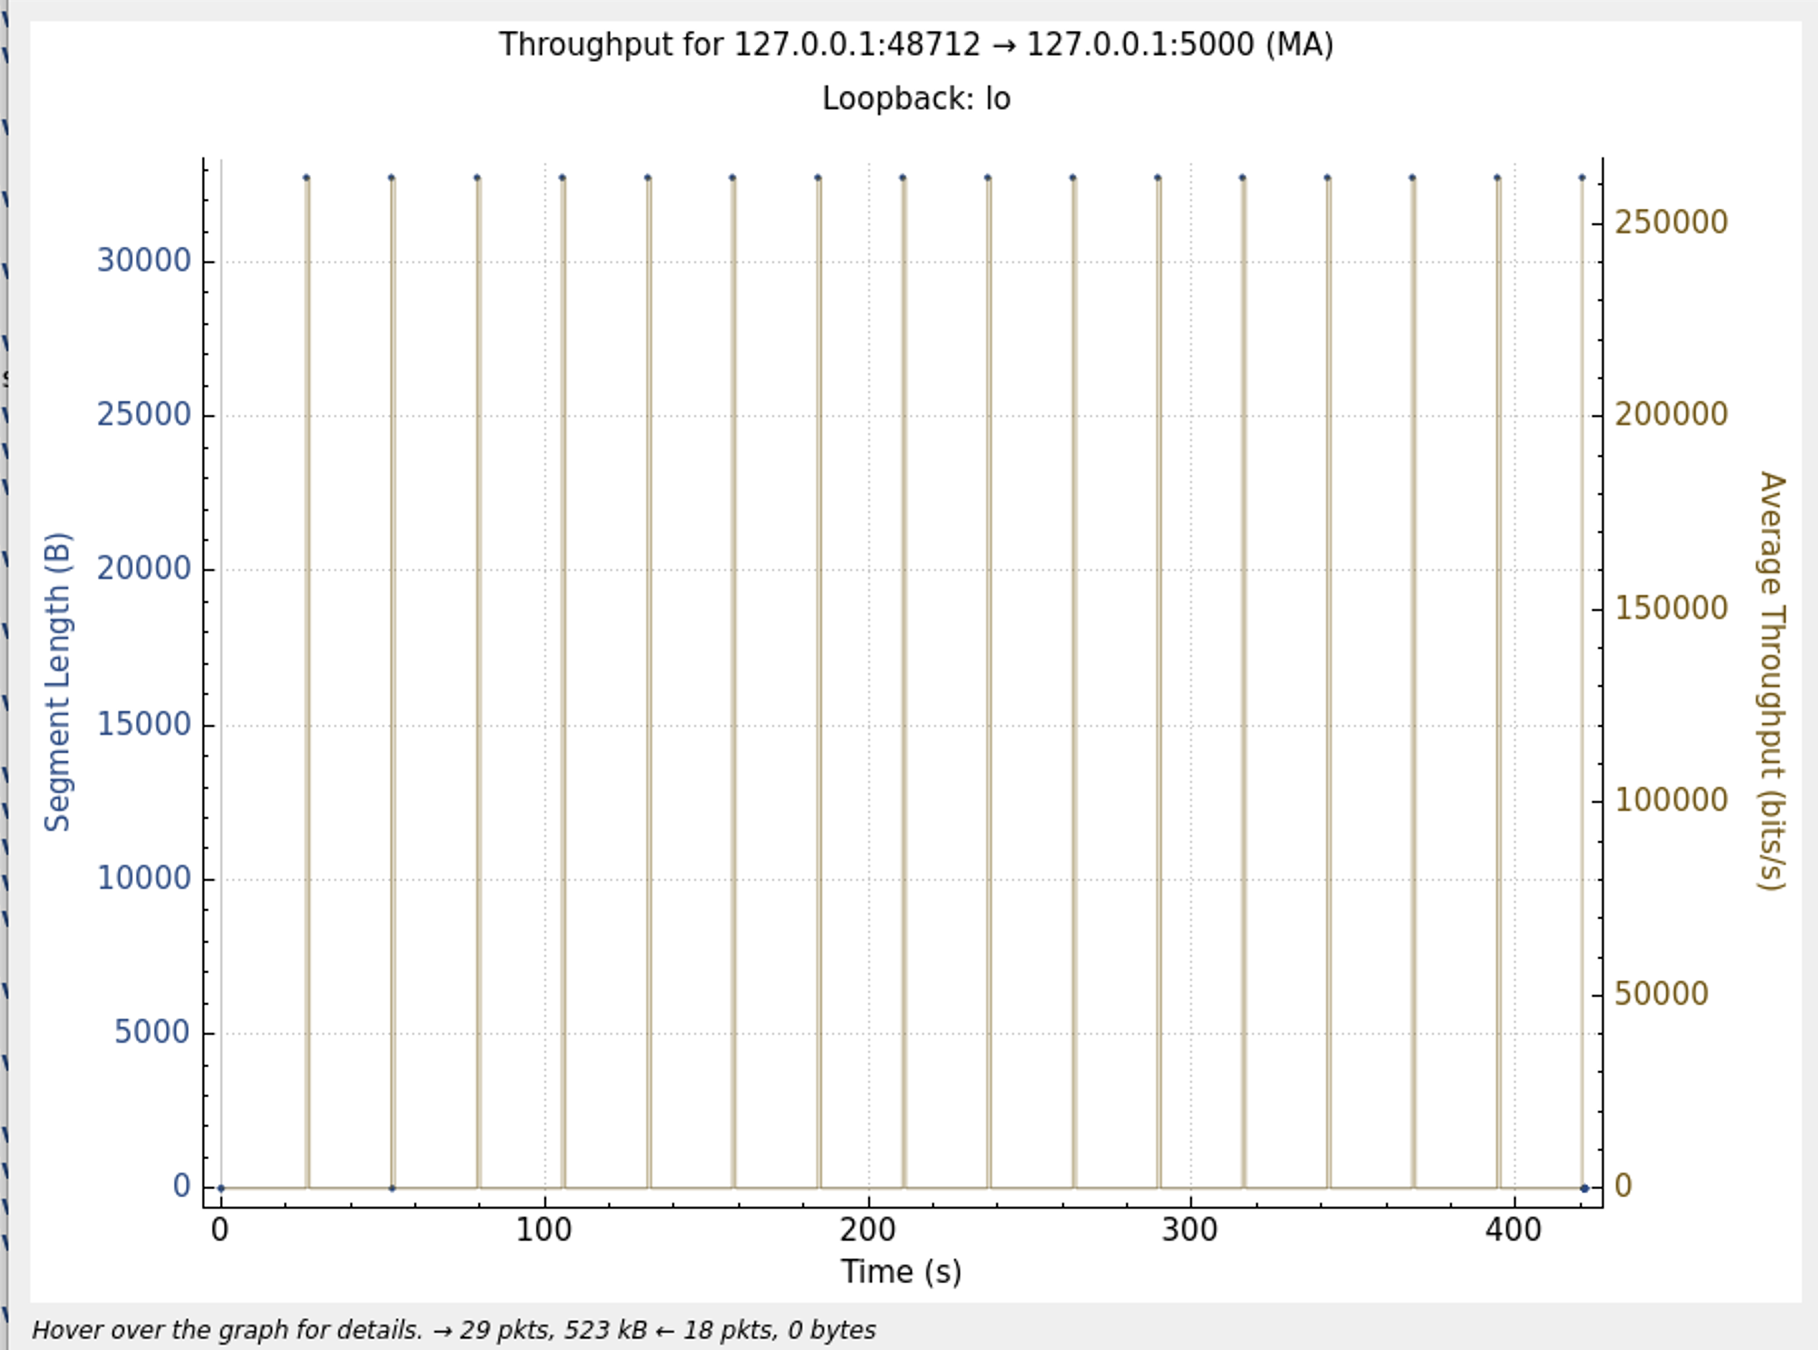
\includegraphics[width=\textwidth]{Pics/Cubic/r10kbit_s1m_th}
        \caption{10 kbit rate. BORKED}
    \end{subfigure}
    \caption{Comparison of the throughput for 1mbit of data sent with different rate limits.}
    \label{fig:four_images}
\end{figure}

It is to be noted that with a rate of 10kb, even after more than one hour only about half of the data was sent. At which point I opted to stop the scripts.\\
I think the development of the window scaling, which gives a good understanding of the congestion window, is clearly visible in figure 5. We can see the window ramping up initially, reaching a maximum of roughly 30K, shrinking down when packets are dropped and then ramping up again afterwards. The figure 6 b, showcase a very high throughput utilization even when the window shrinks.\\
Experimenting with this first congestion control algorithm I have figured out that smaller data sent sizes do not produce very indicative results. Consequently for the next congestion control algorithm I have only tested size of 50kb, 100kb and 1mb. Also I have experienced a daunting slowness with data of 1mb and rate of 10Kb, therefore I will avoid this combination of settings for the next algorithms.

\subsection*{Reno}
Given what I have learned experimenting with the previous algorithm I have used data sizes of 50kb, 100kb and 1mb. I will discuss the results that I found the most interesting but all of the rtt, throughput and window scaling I have obtained are available on github in the folder pdf/Pics/Reno.\\
It seemed to me that Reno was slower than Cubic, in most test it seemed to me to have had to wait longer for the transmission of all the bytes. This might be only an impression though.\\
\begin{figure}[H]
    \centering
    \begin{subfigure}[b]{0.45\textwidth}
        \centering
        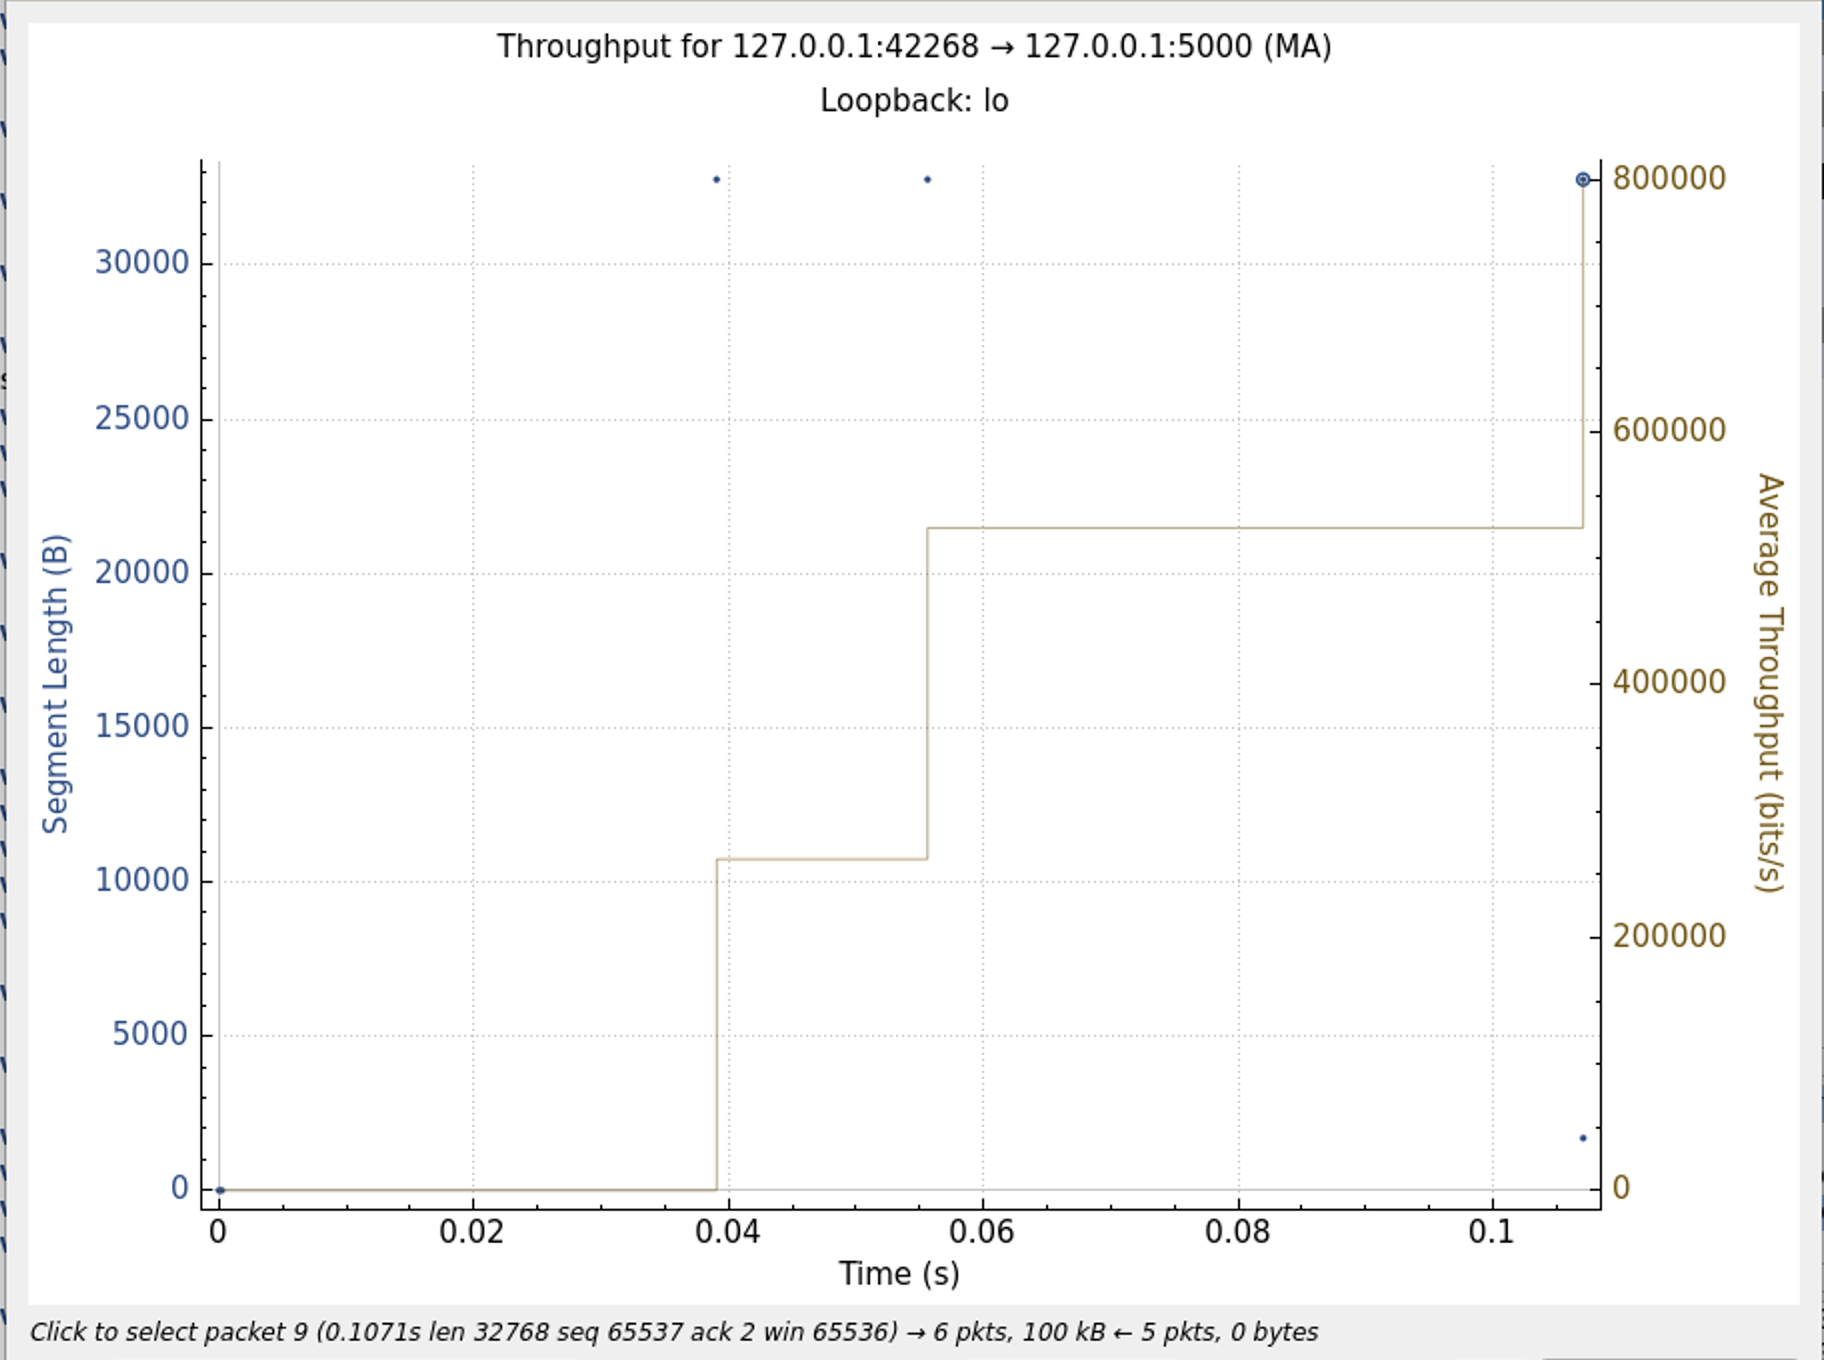
\includegraphics[width=\textwidth]{Pics/Reno/r10mbit_s100k_th}
        \caption{10 mbit rate}
    \end{subfigure}
    \hfill
    \begin{subfigure}[b]{0.45\textwidth}
        \centering
        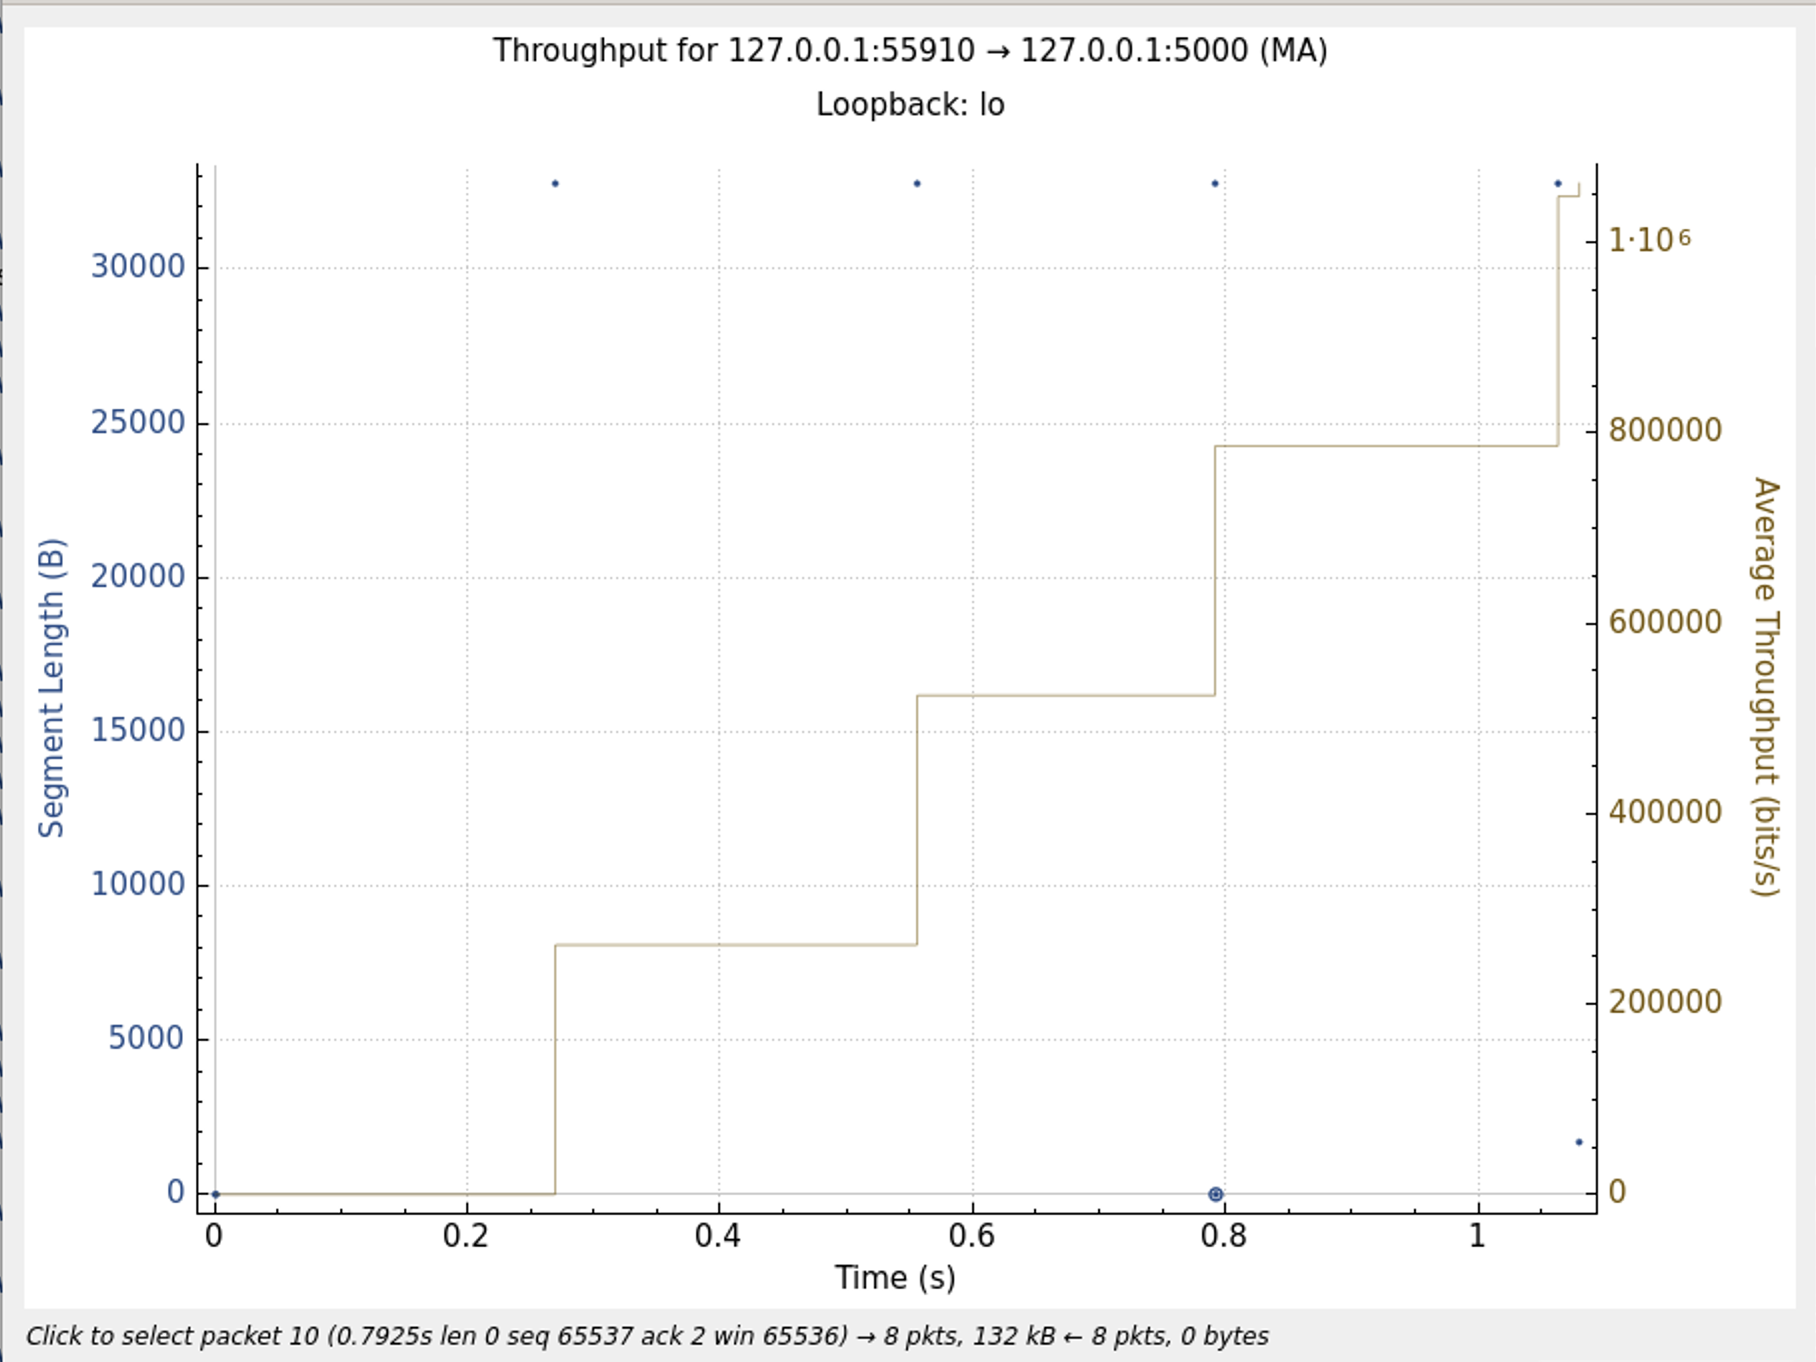
\includegraphics[width=\textwidth]{Pics/Reno/r1mbit_s100k_th}
        \caption{1 mbit rate}
    \end{subfigure}
    \medskip

    \begin{subfigure}[b]{0.45\textwidth}
        \centering
        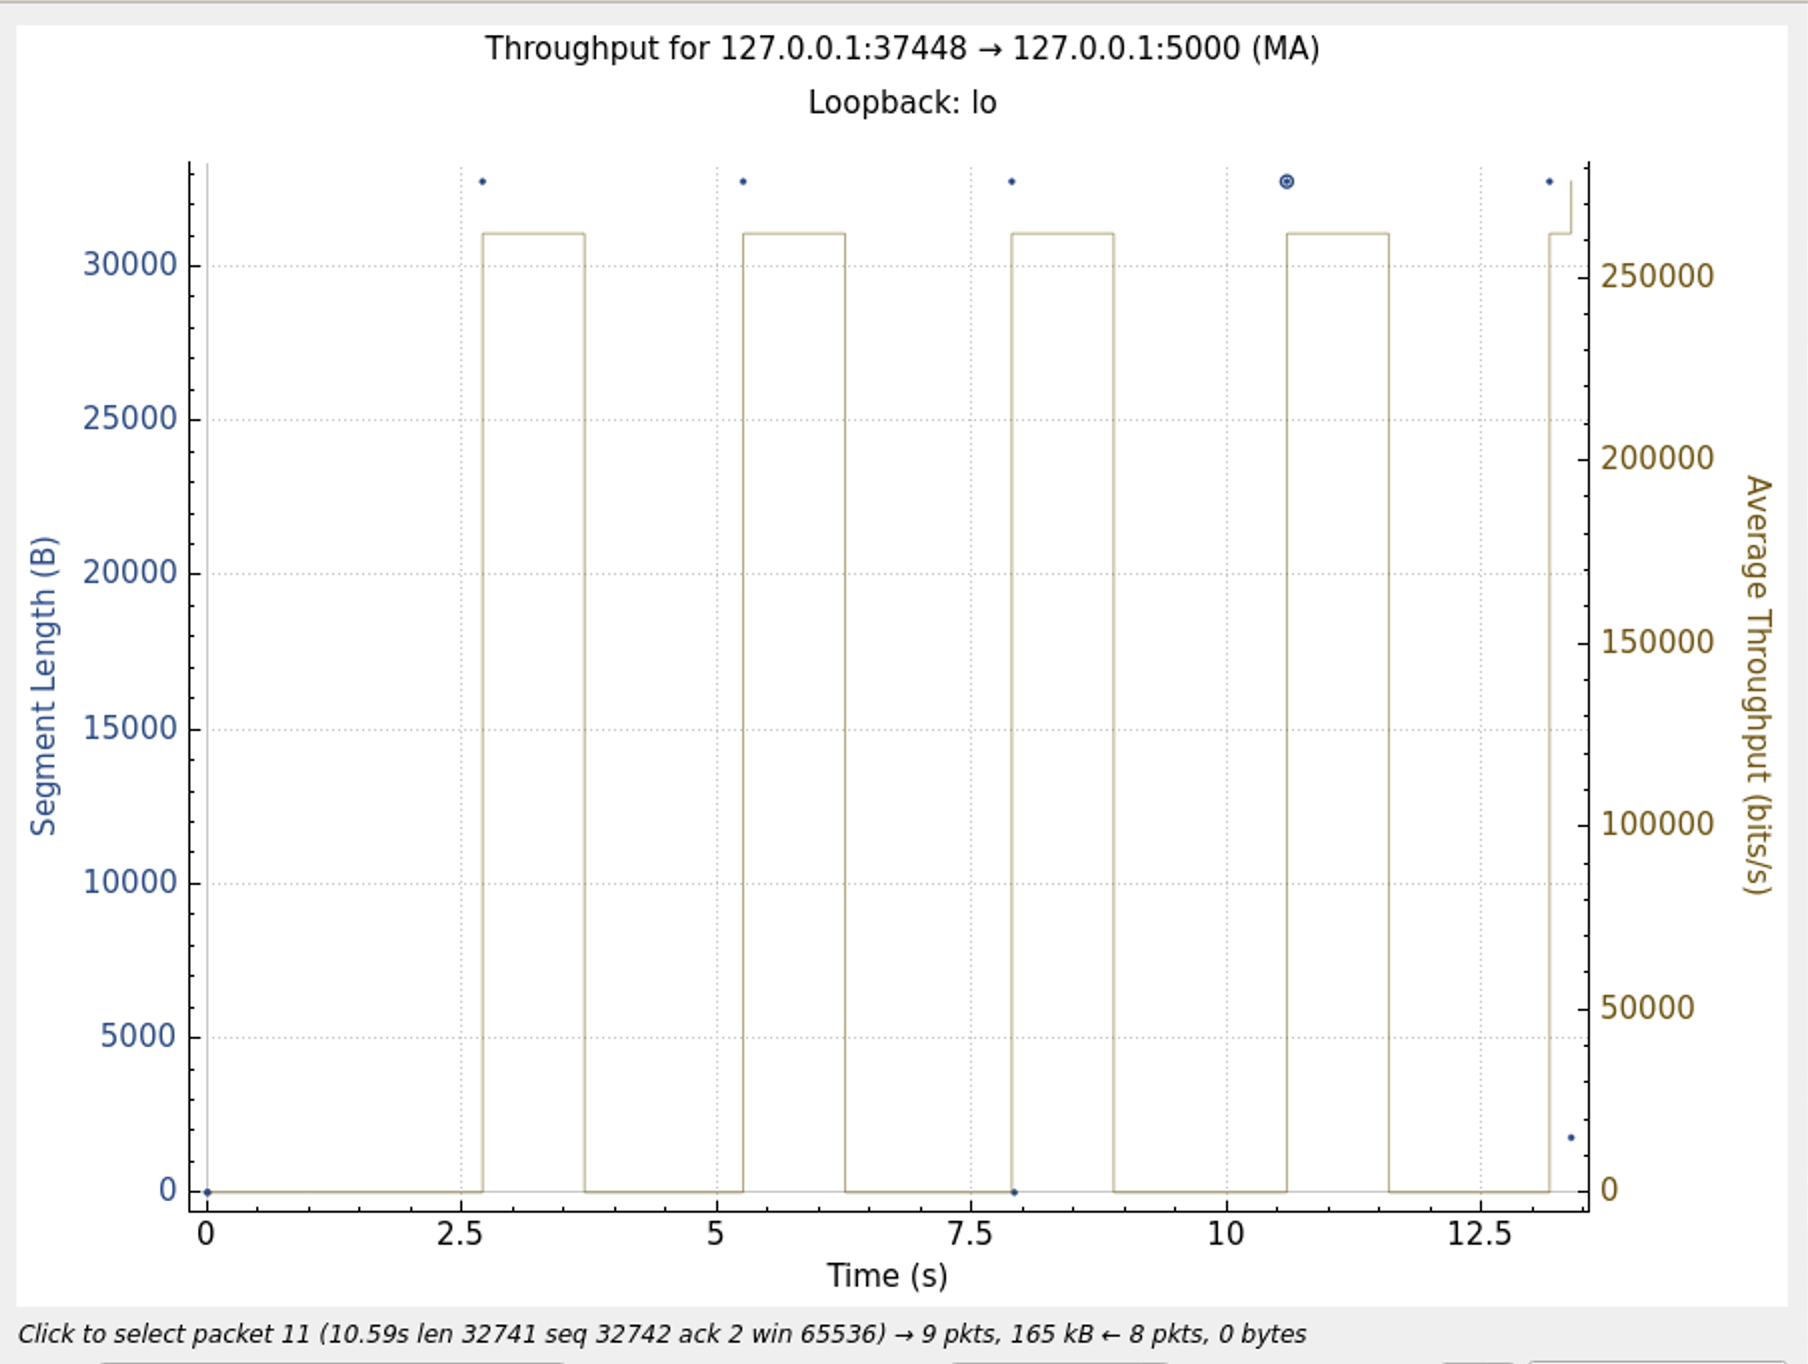
\includegraphics[width=\textwidth]{Pics/Reno/r100kbit_s100k_th}
        \caption{100 kbit rate}
    \end{subfigure}
    \hfill
    \begin{subfigure}[b]{0.45\textwidth}
        \centering
        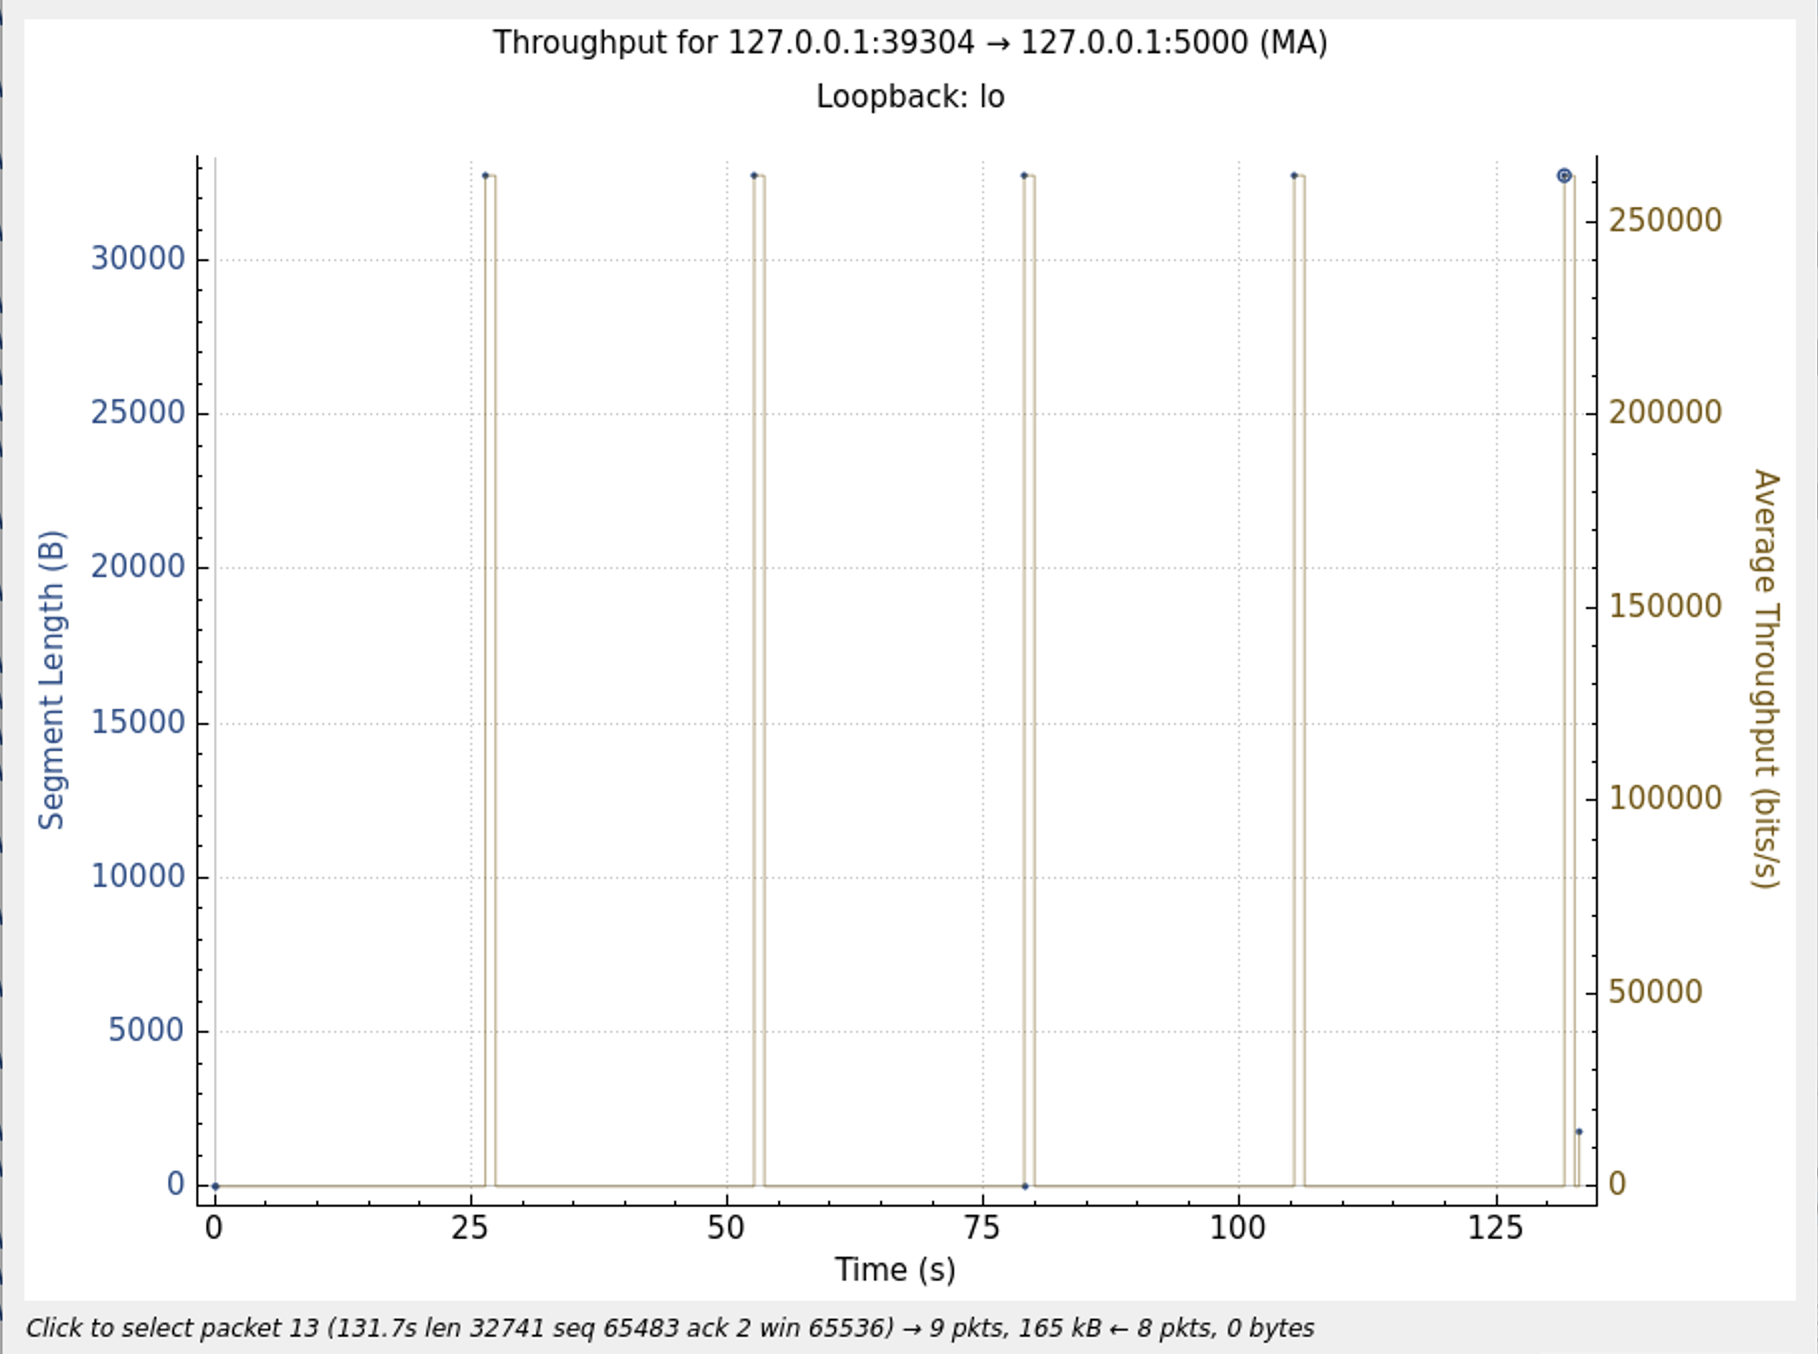
\includegraphics[width=\textwidth]{Pics/Reno/r10kbit_s100k_th}
        \caption{10 kbit rate}
    \end{subfigure}
    \caption{Comparison of the throughput for 100kbit of data sent with different rate limits. Reno}
    \label{fig:four_images}
\end{figure}

\begin{figure}[H]
    \centering
    \begin{subfigure}[b]{0.45\textwidth}
        \centering
        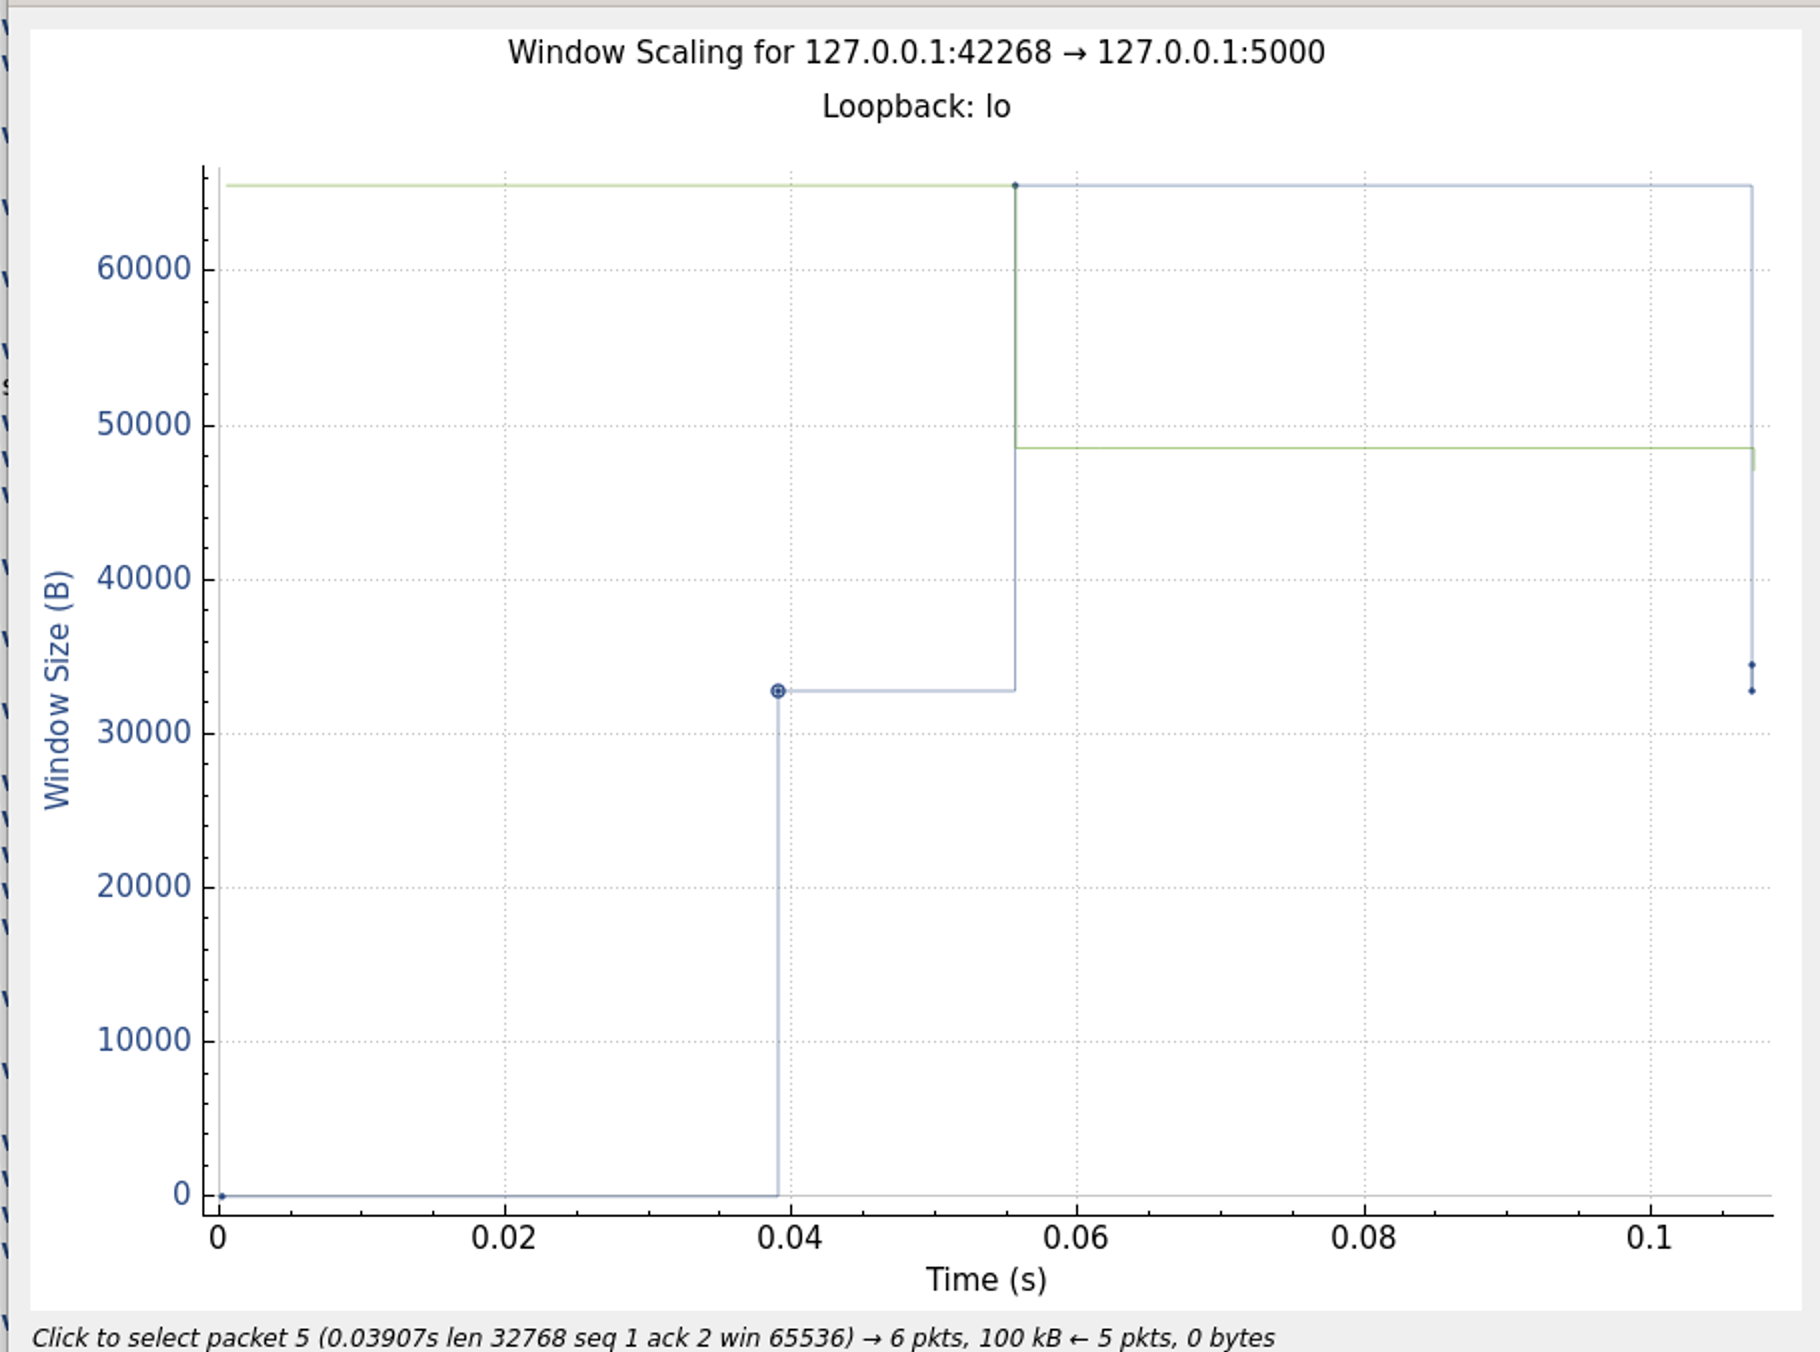
\includegraphics[width=\textwidth]{Pics/Reno/r10mbit_s100k_ws}
        \caption{10 mbit rate}
    \end{subfigure}
    \hfill
    \begin{subfigure}[b]{0.45\textwidth}
        \centering
        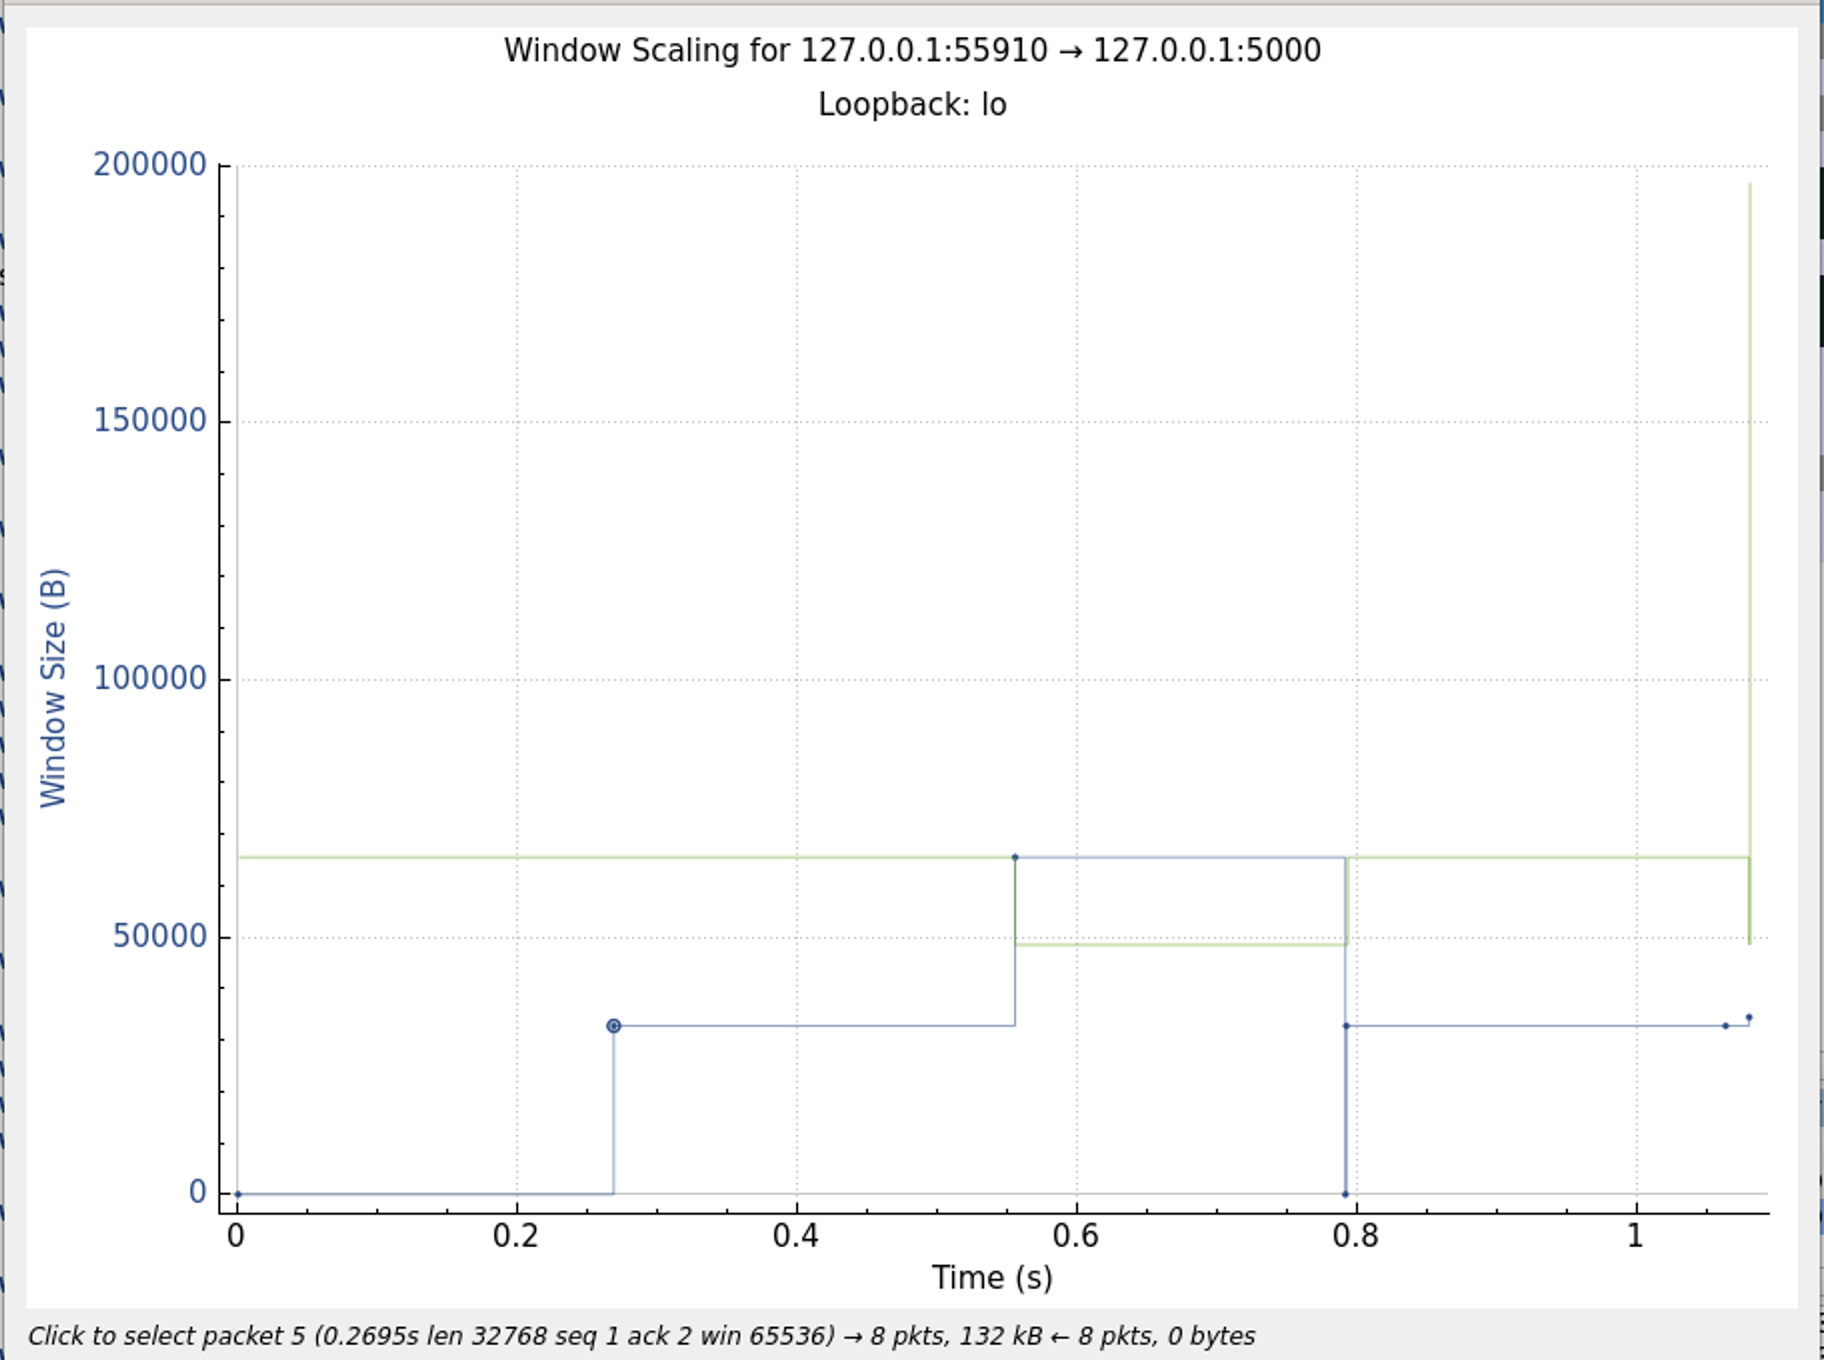
\includegraphics[width=\textwidth]{Pics/Reno/r1mbit_s100k_ws}
        \caption{1 mbit rate }
    \end{subfigure}
    \medskip

    \begin{subfigure}[b]{0.45\textwidth}
        \centering
        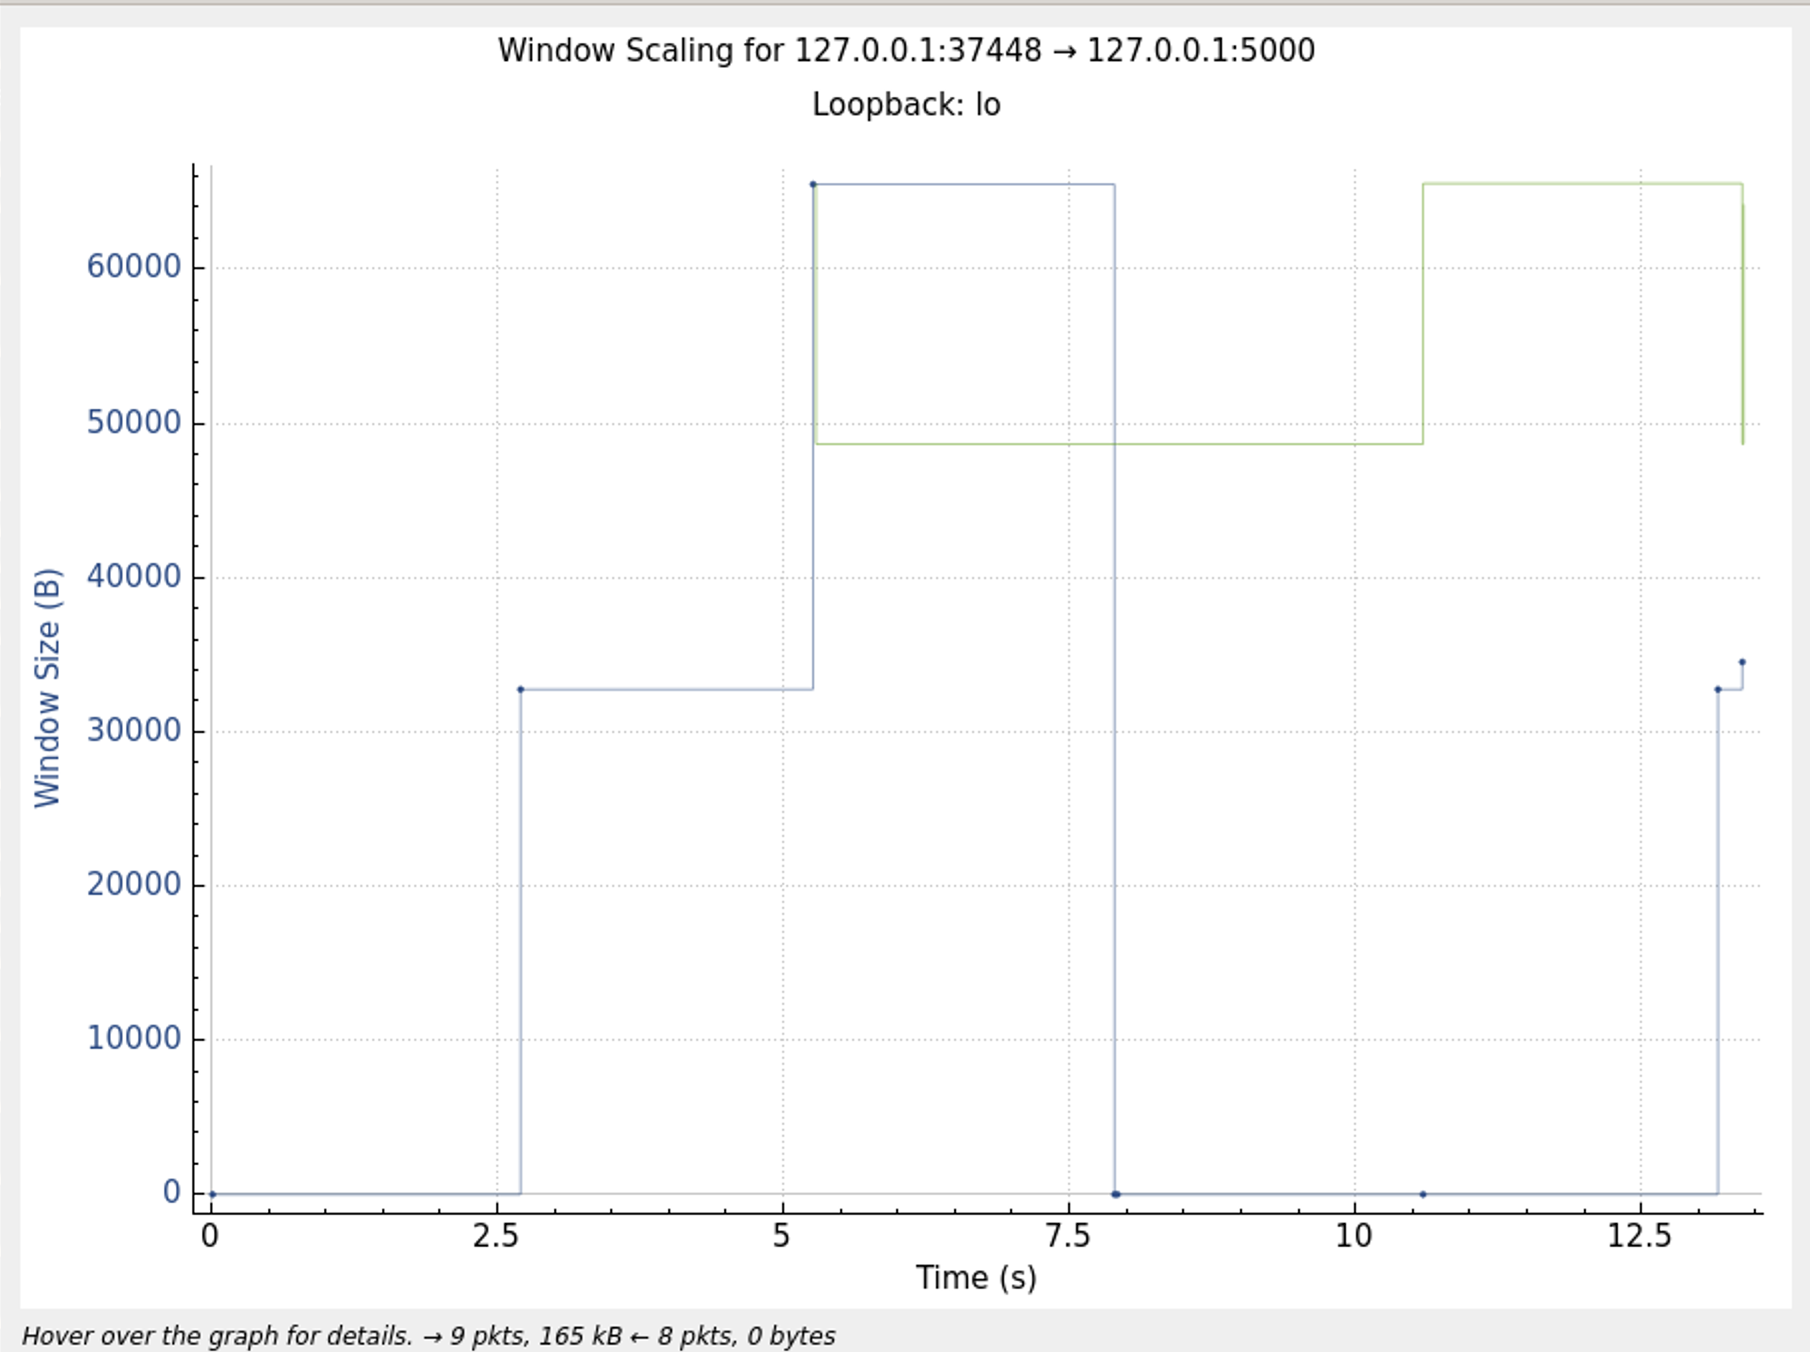
\includegraphics[width=\textwidth]{Pics/Reno/r100kbit_s100k_ws}
        \caption{100 kbit rate}
    \end{subfigure}
    \hfill
    \begin{subfigure}[b]{0.45\textwidth}
        \centering
        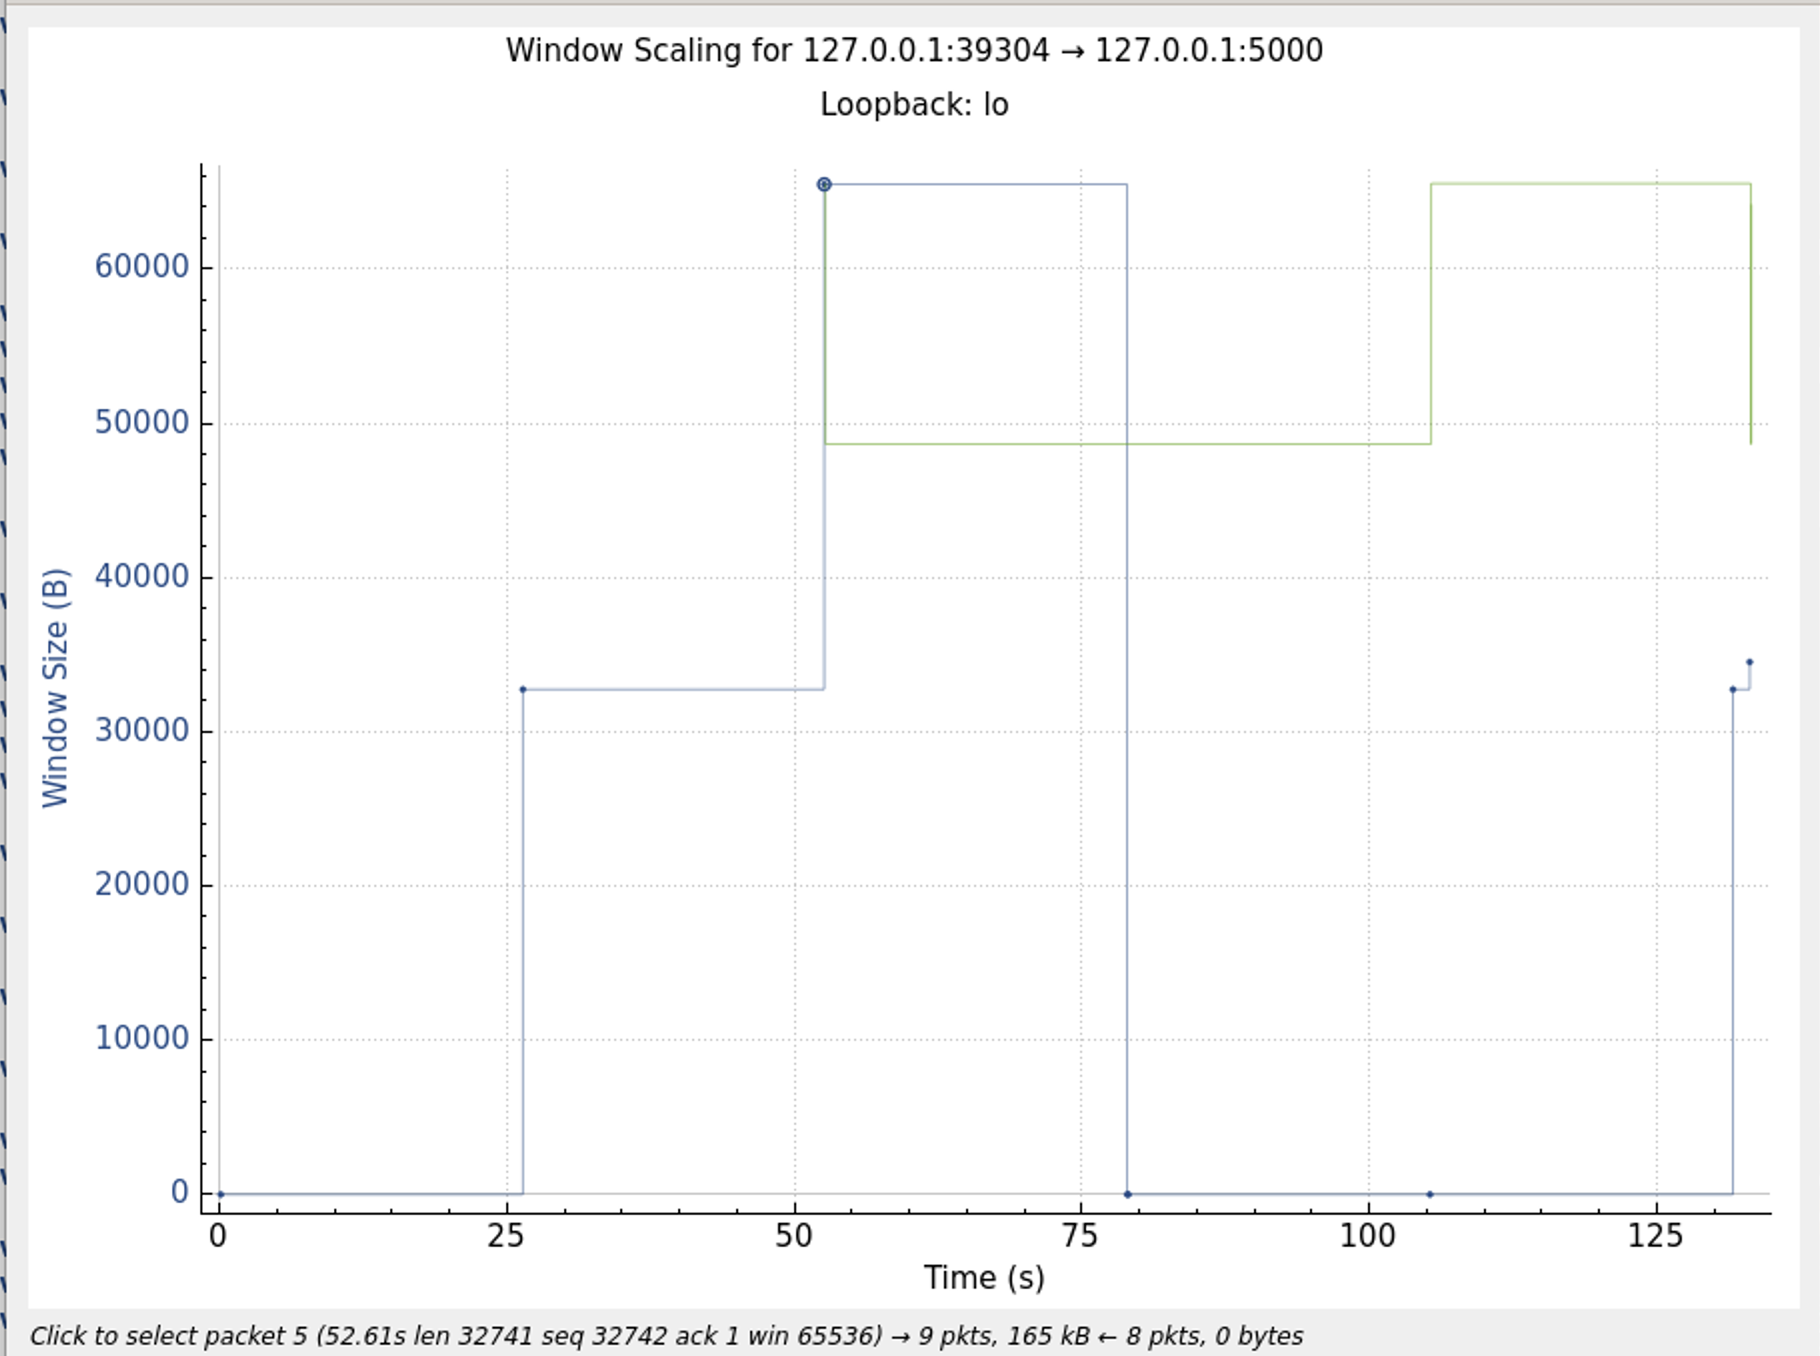
\includegraphics[width=\textwidth]{Pics/Reno/r10kbit_s100k_ws}
        \caption{10 kbit rate}
    \end{subfigure}
    \caption{Comparison of the window scaling for 100kbit of data sent with different rate limits. Reno}
    \label{fig:four_images}
\end{figure}
Comparing figure 8 to figure 3 we can see that the window scaling remains low longer with Reno than with Cubic.\\

\begin{figure}[H]
    \centering
    \begin{subfigure}[b]{0.45\textwidth}
        \centering
        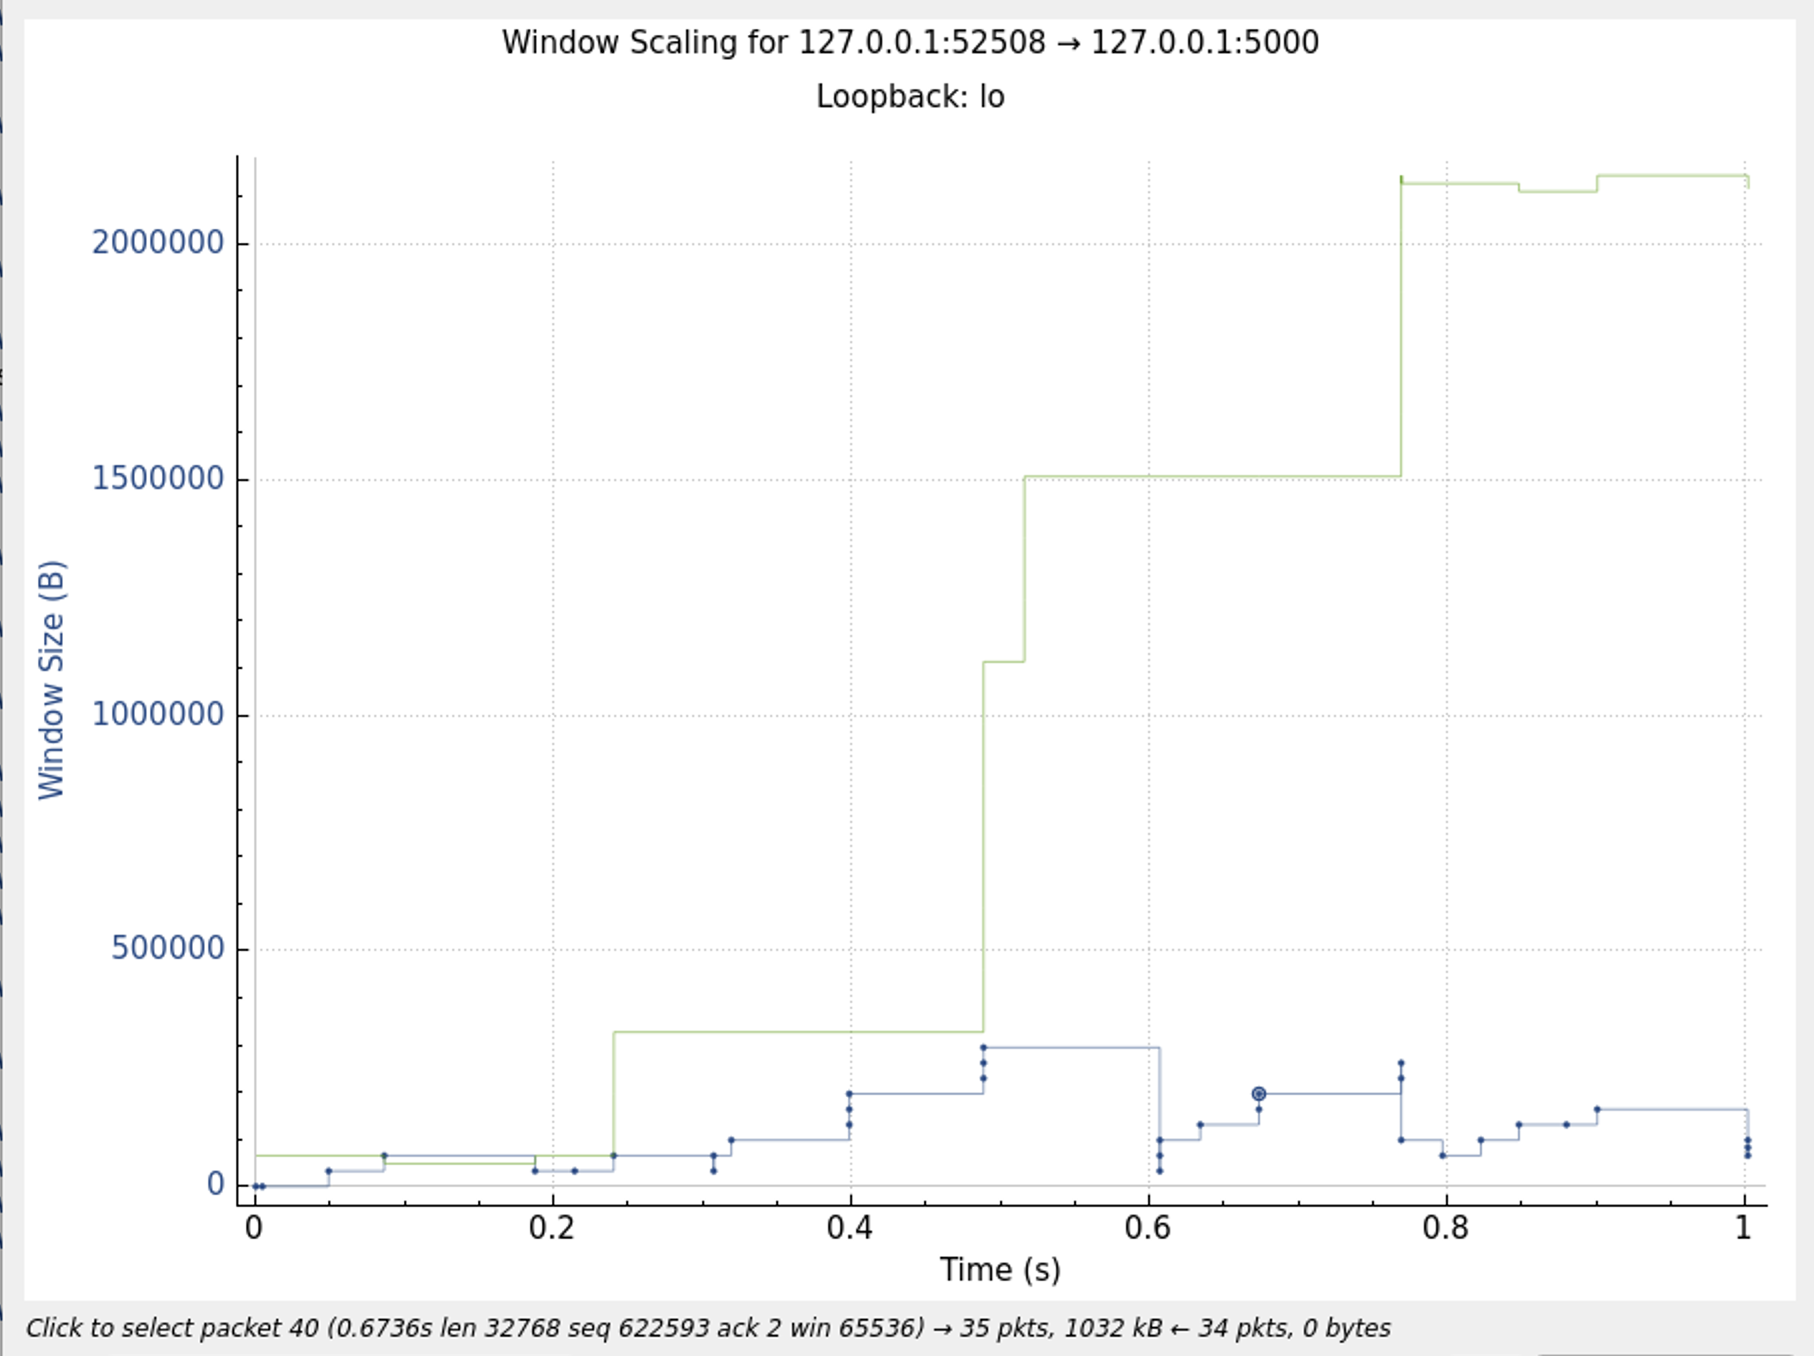
\includegraphics[width=\textwidth]{Pics/Reno/r10mbit_s1m_ws}
        \caption{10 mbit rate }
    \end{subfigure}
    \hfill
    \begin{subfigure}[b]{0.45\textwidth}
        \centering
        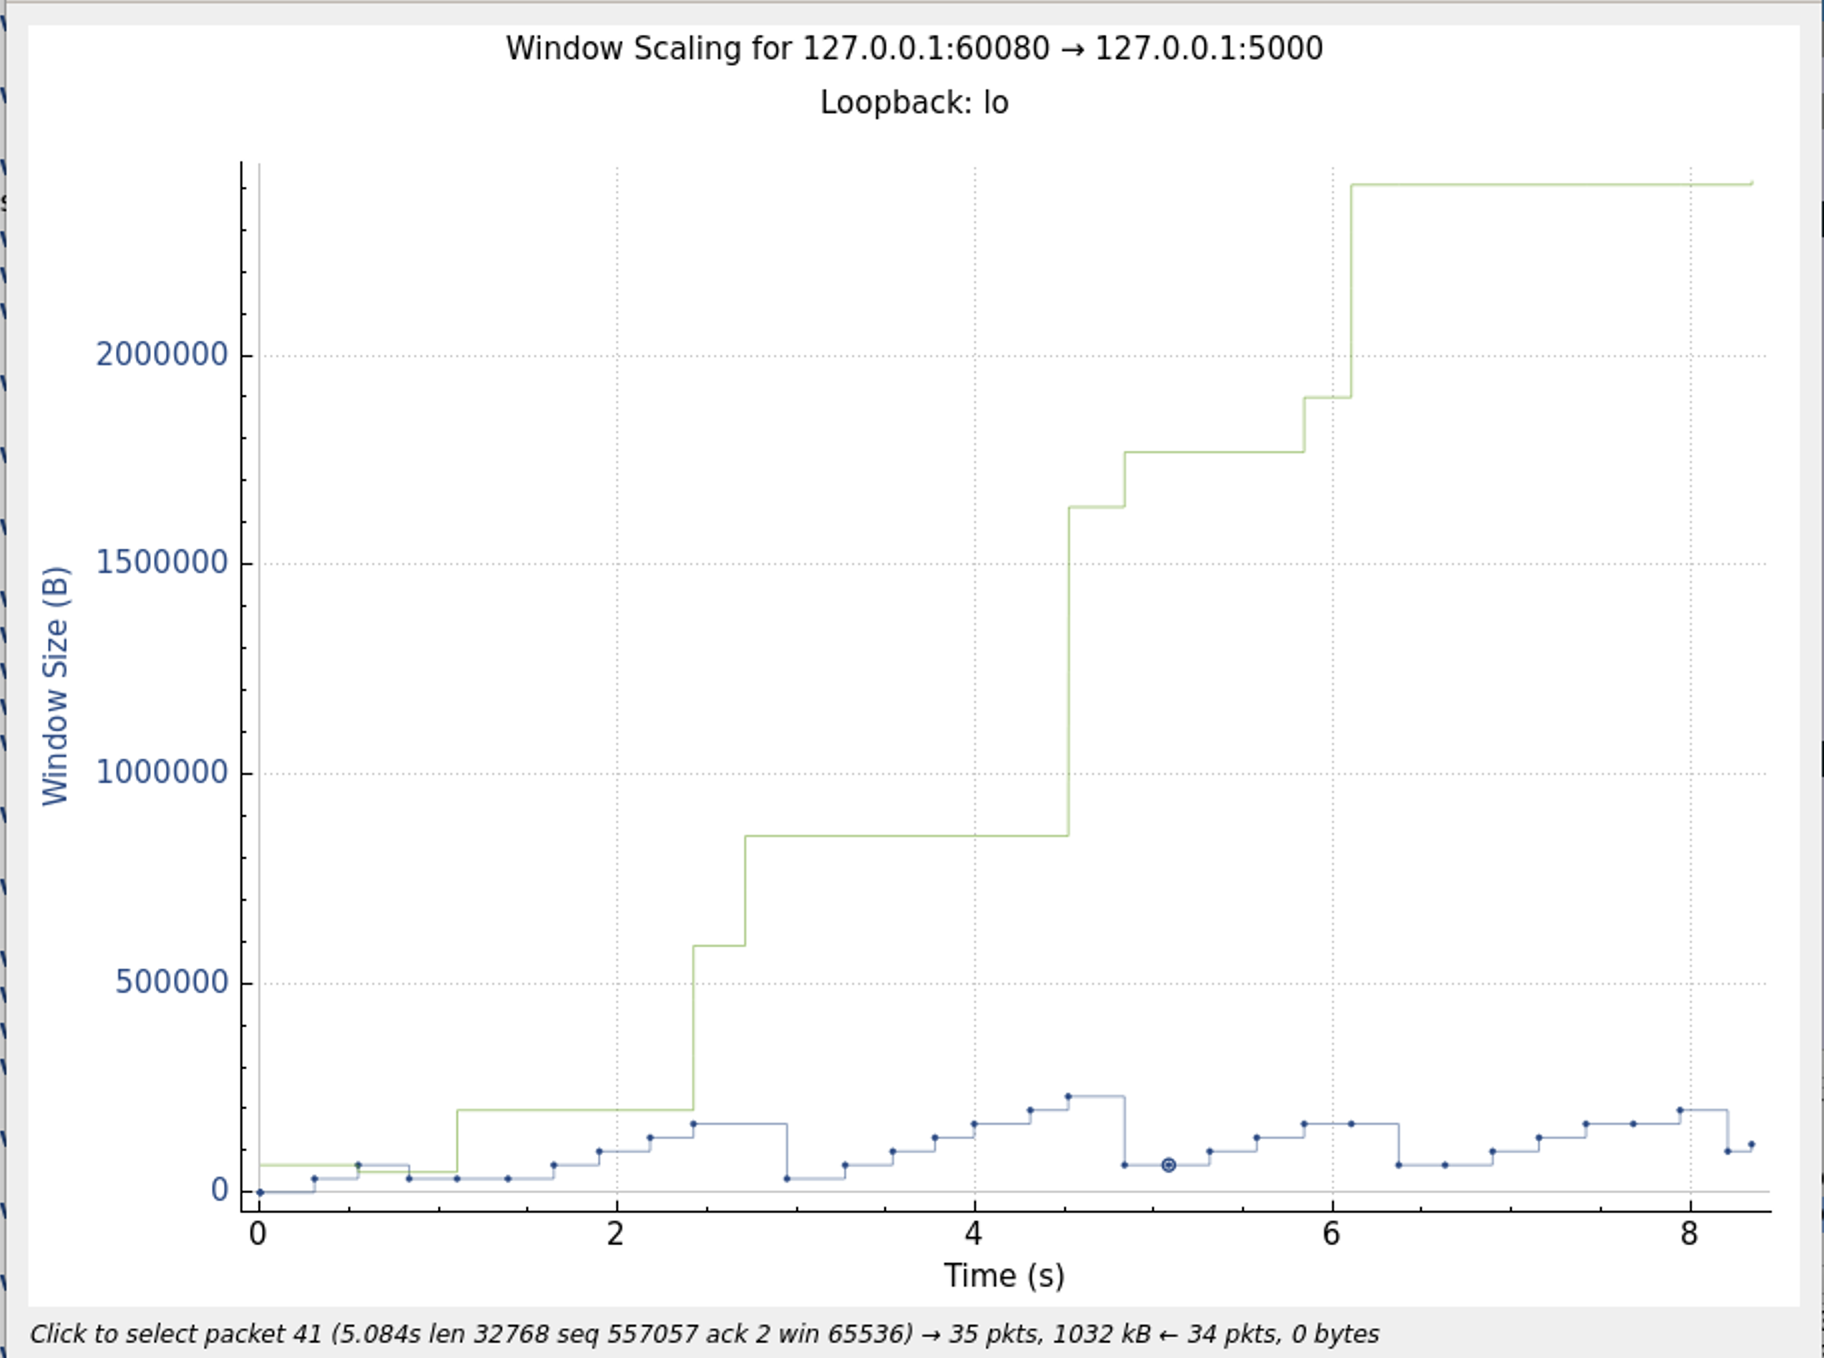
\includegraphics[width=\textwidth]{Pics/Reno/r1mbit_s1m_ws}
        \caption{1 mbit rate}
    \end{subfigure}
    \medskip

    \begin{subfigure}[b]{0.45\textwidth}
        \centering
        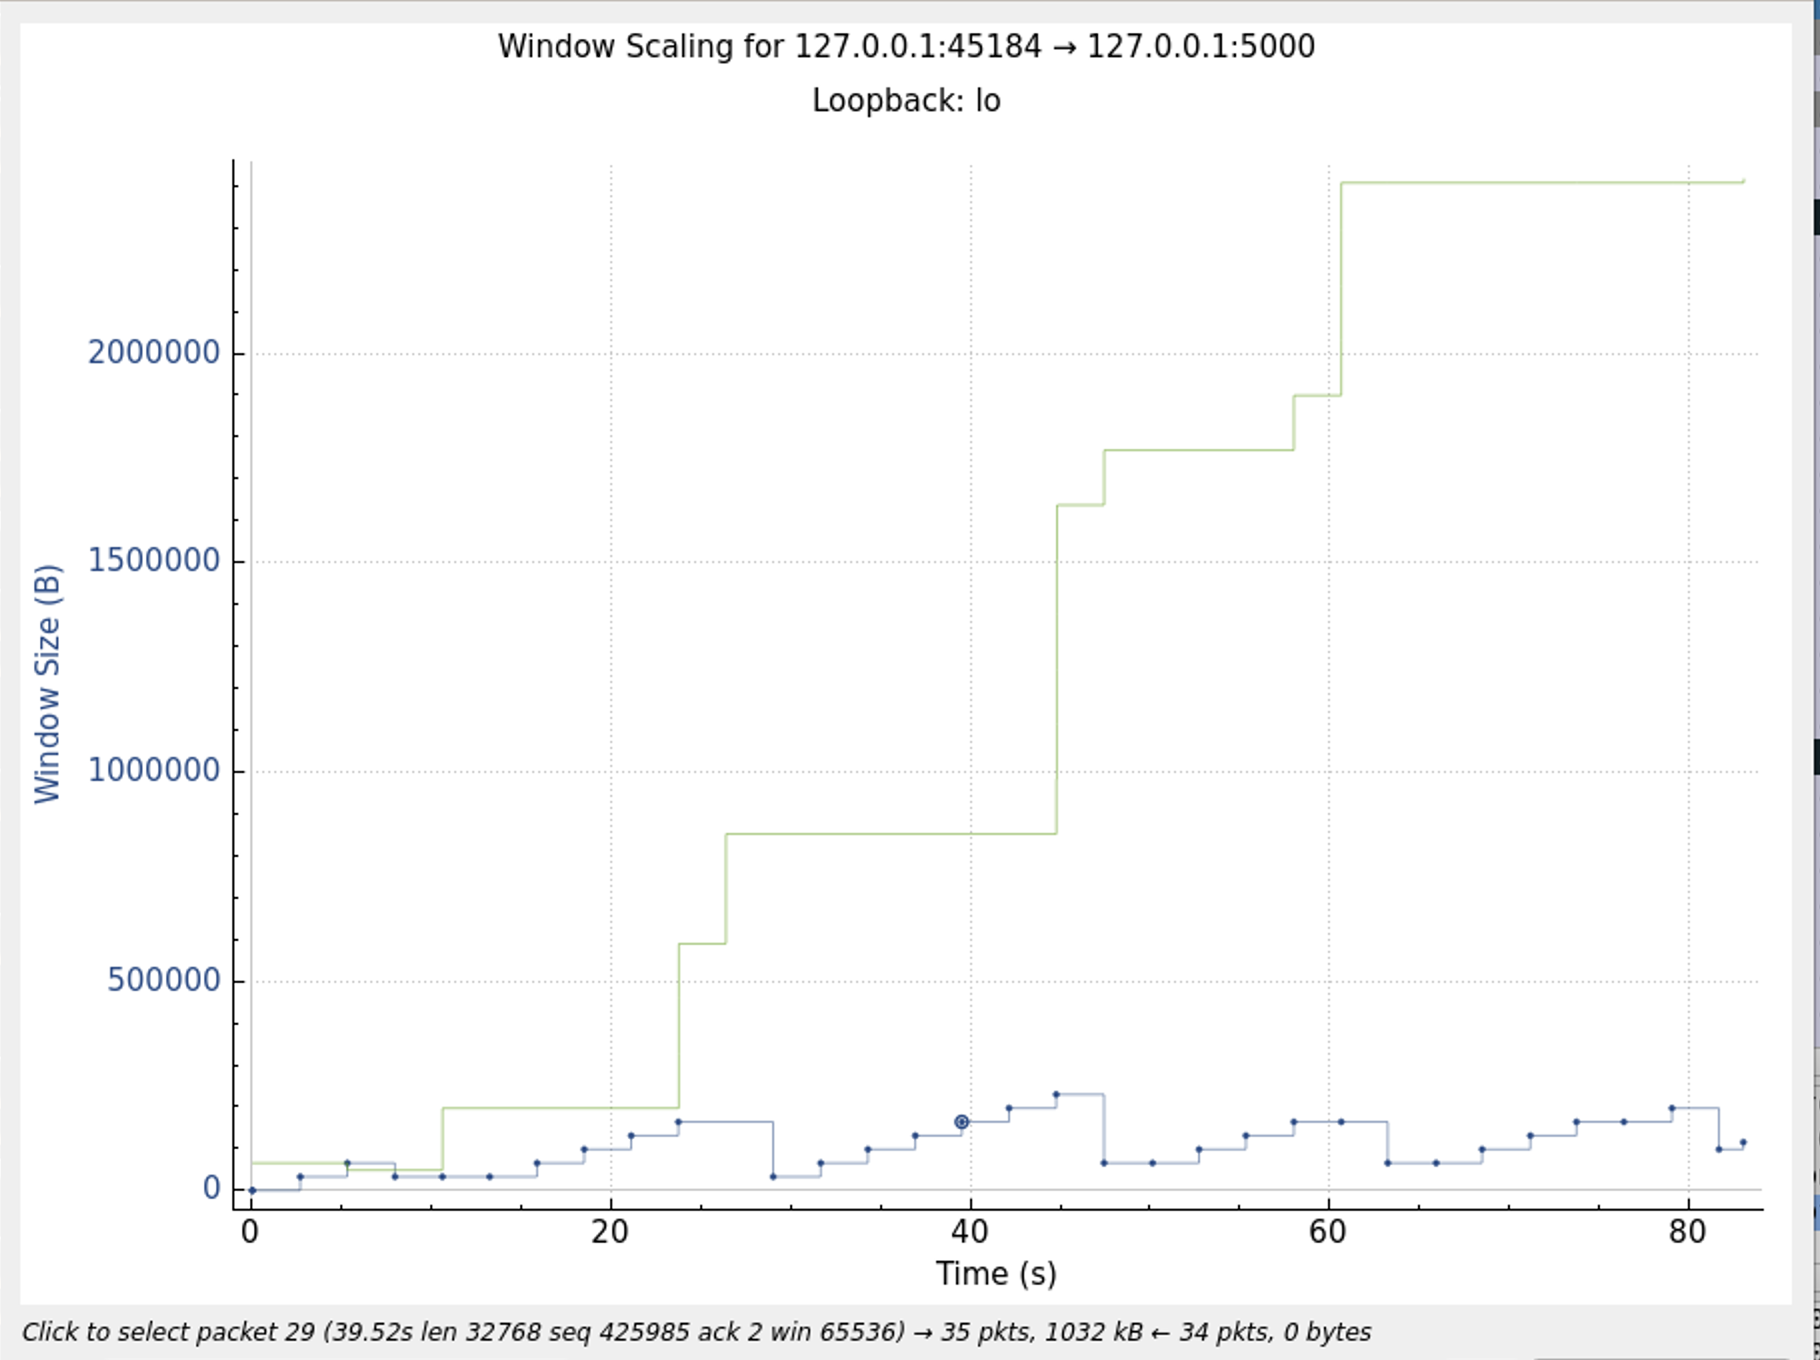
\includegraphics[width=\textwidth]{Pics/Reno/r100kbit_s1m_ws}
        \caption{100 kbit rate}
    \end{subfigure}
    \hfill
    \begin{subfigure}[b]{0.45\textwidth}
        \centering
        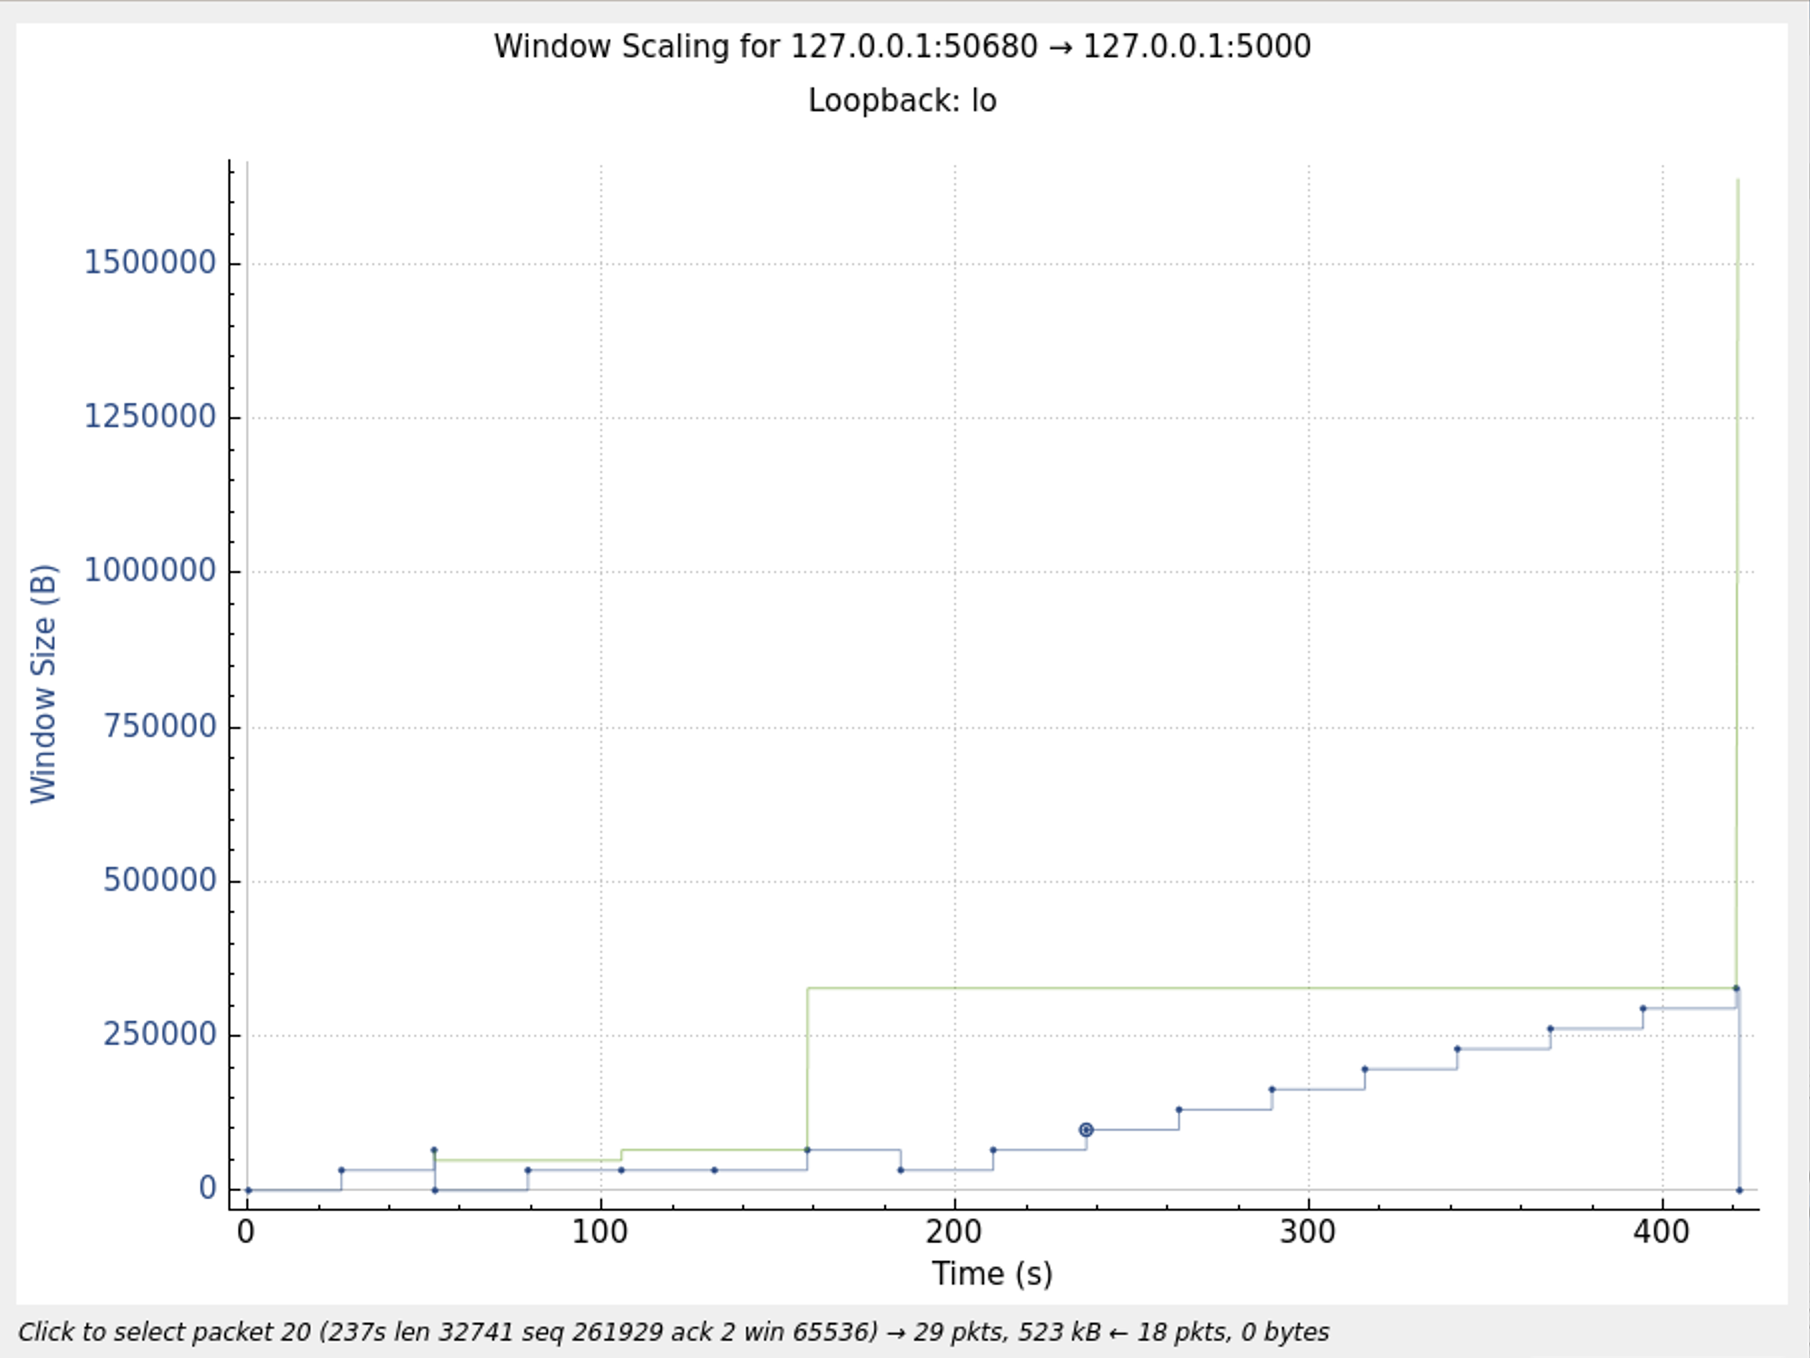
\includegraphics[width=\textwidth]{Pics/Reno/r10kbit_s1m_ws}
        \caption{10 kbit rate. BORKED}
    \end{subfigure}
    \caption{Comparison of the window scaling for 1mbit of data sent with different rate limits. Reno}
    \label{fig:four_images}
\end{figure}

\begin{figure}[H]
    \centering
    \begin{subfigure}[b]{0.45\textwidth}
        \centering
        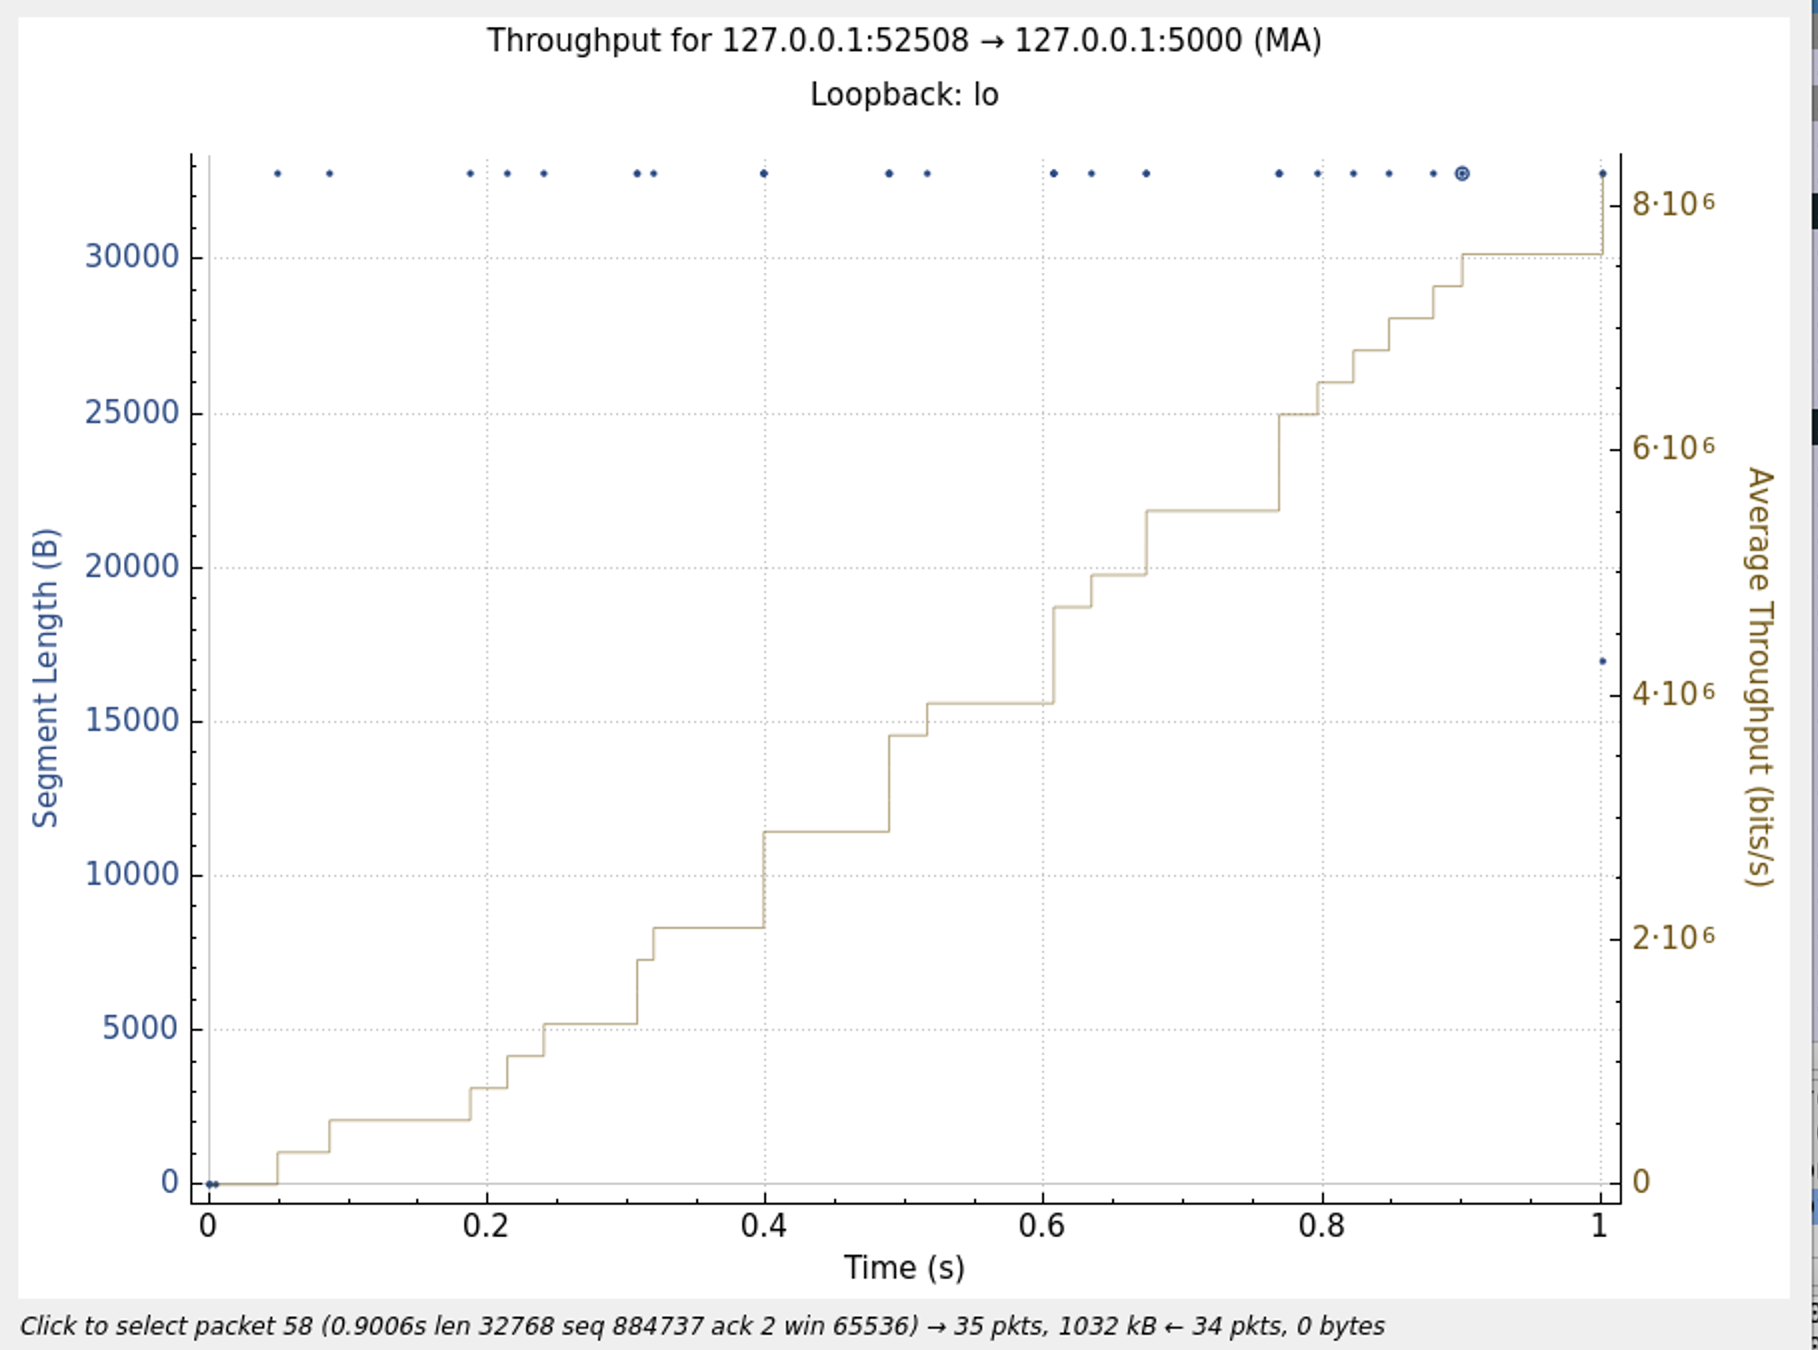
\includegraphics[width=\textwidth]{Pics/Reno/r10mbit_s1m_th}
        \caption{10 mbit rate}
    \end{subfigure}
    \hfill
    \begin{subfigure}[b]{0.45\textwidth}
        \centering
        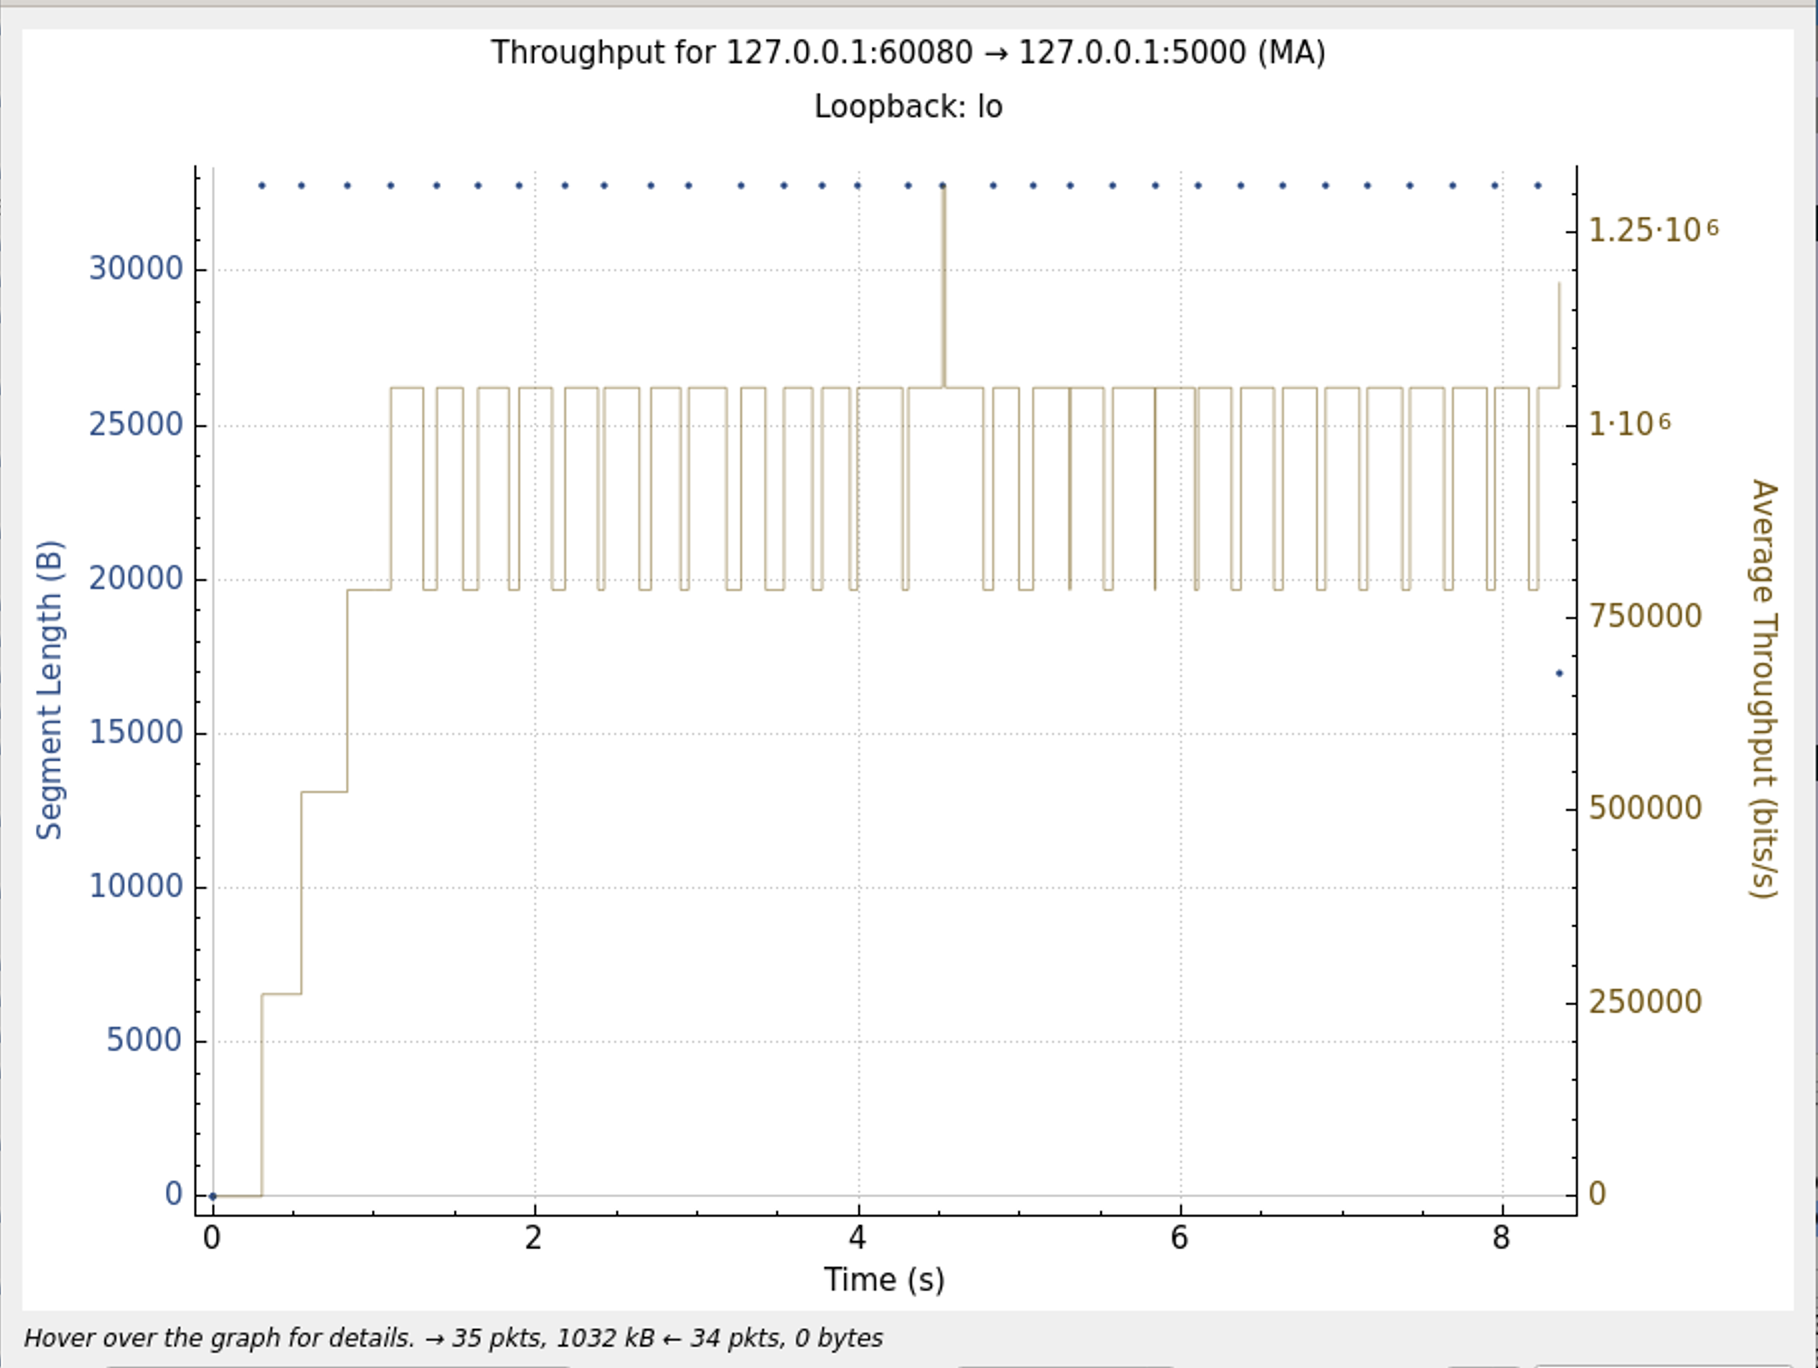
\includegraphics[width=\textwidth]{Pics/Reno/r1mbit_s1m_th}
        \caption{1 mbit rate}
    \end{subfigure}
    \medskip

    \begin{subfigure}[b]{0.45\textwidth}
        \centering
        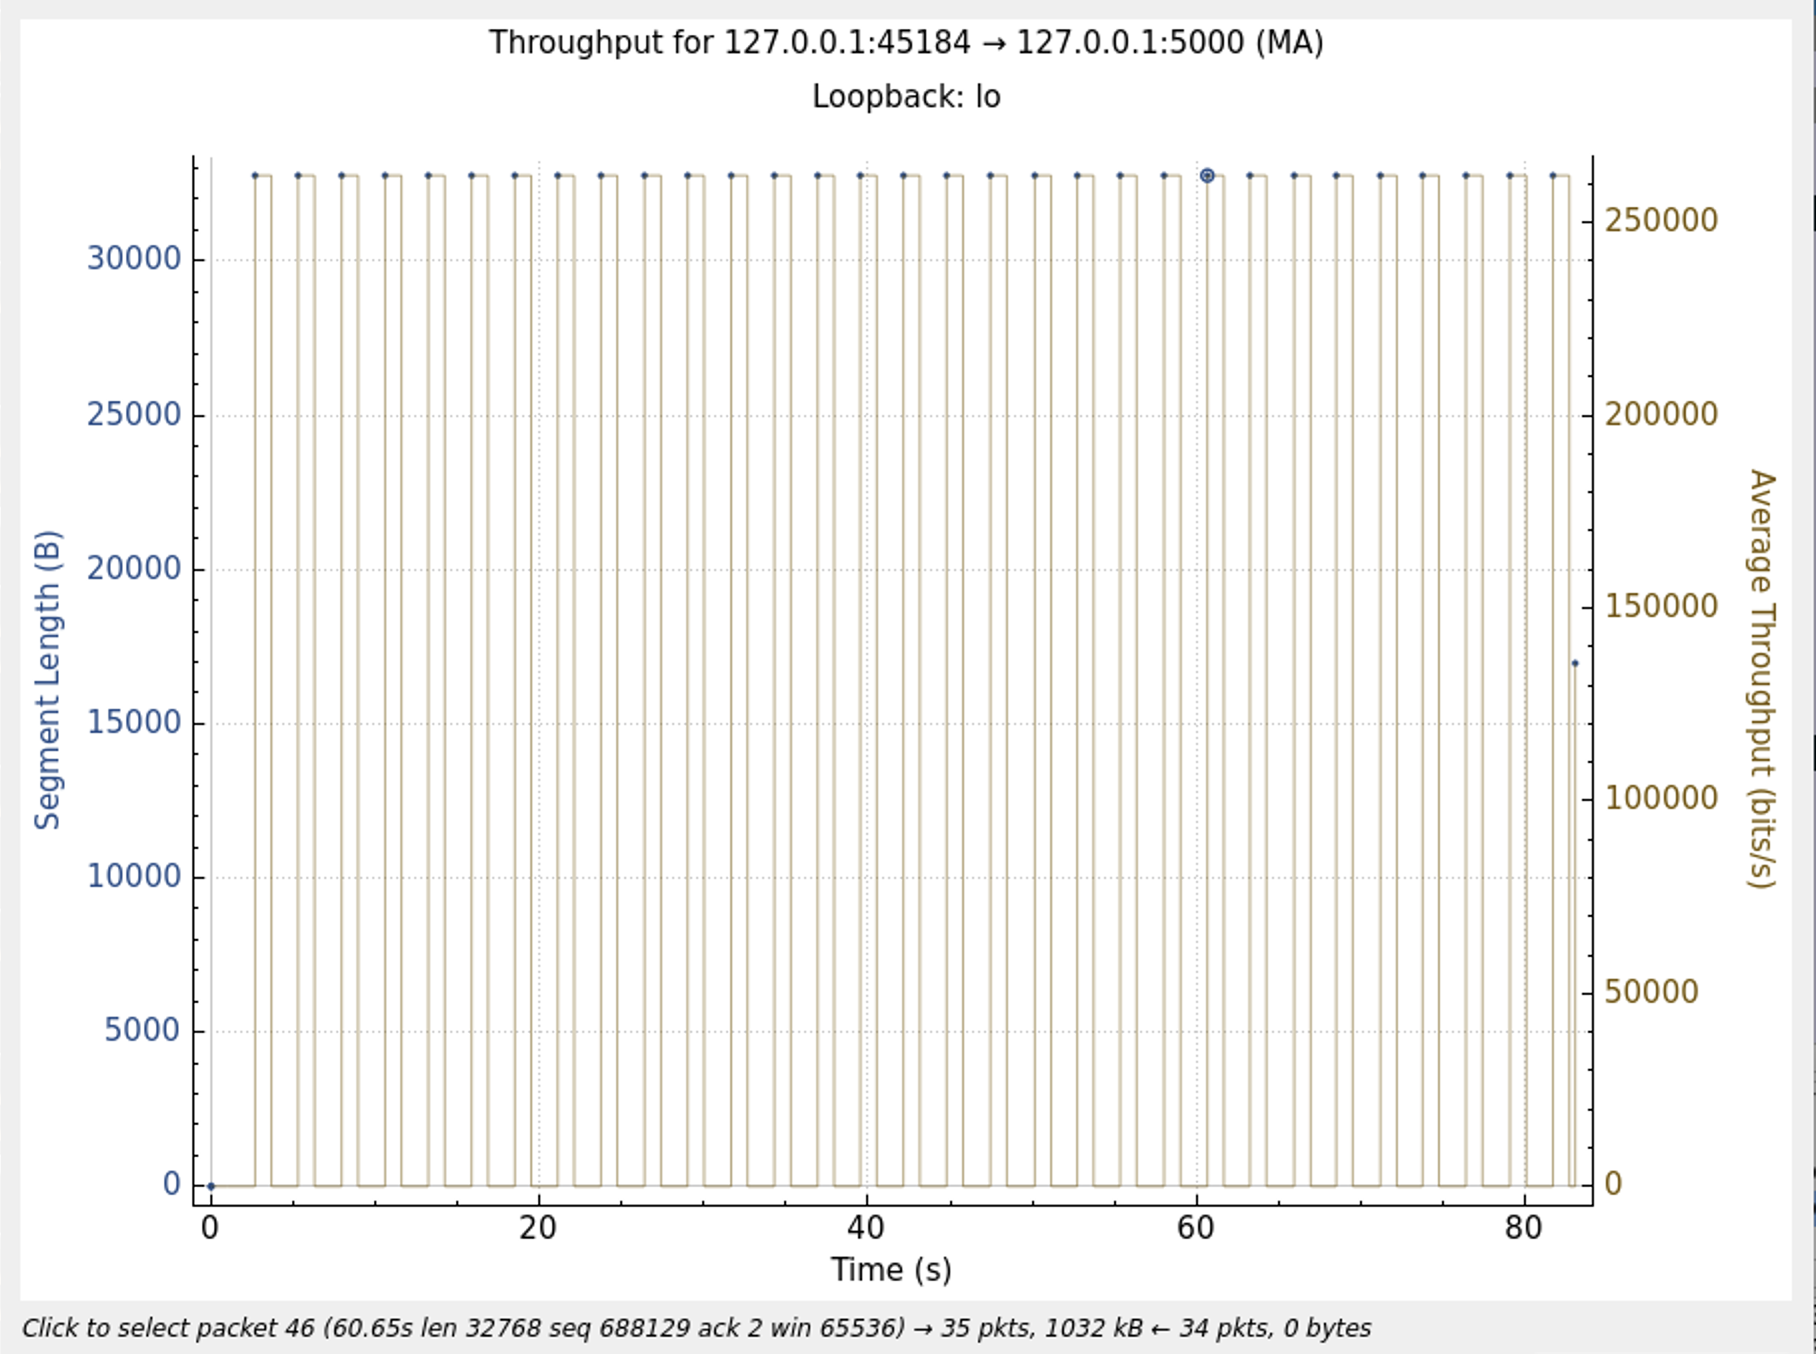
\includegraphics[width=\textwidth]{Pics/Reno/r100kbit_s1m_th}
        \caption{100 kbit rate}
    \end{subfigure}
    \hfill
    \begin{subfigure}[b]{0.45\textwidth}
        \centering
        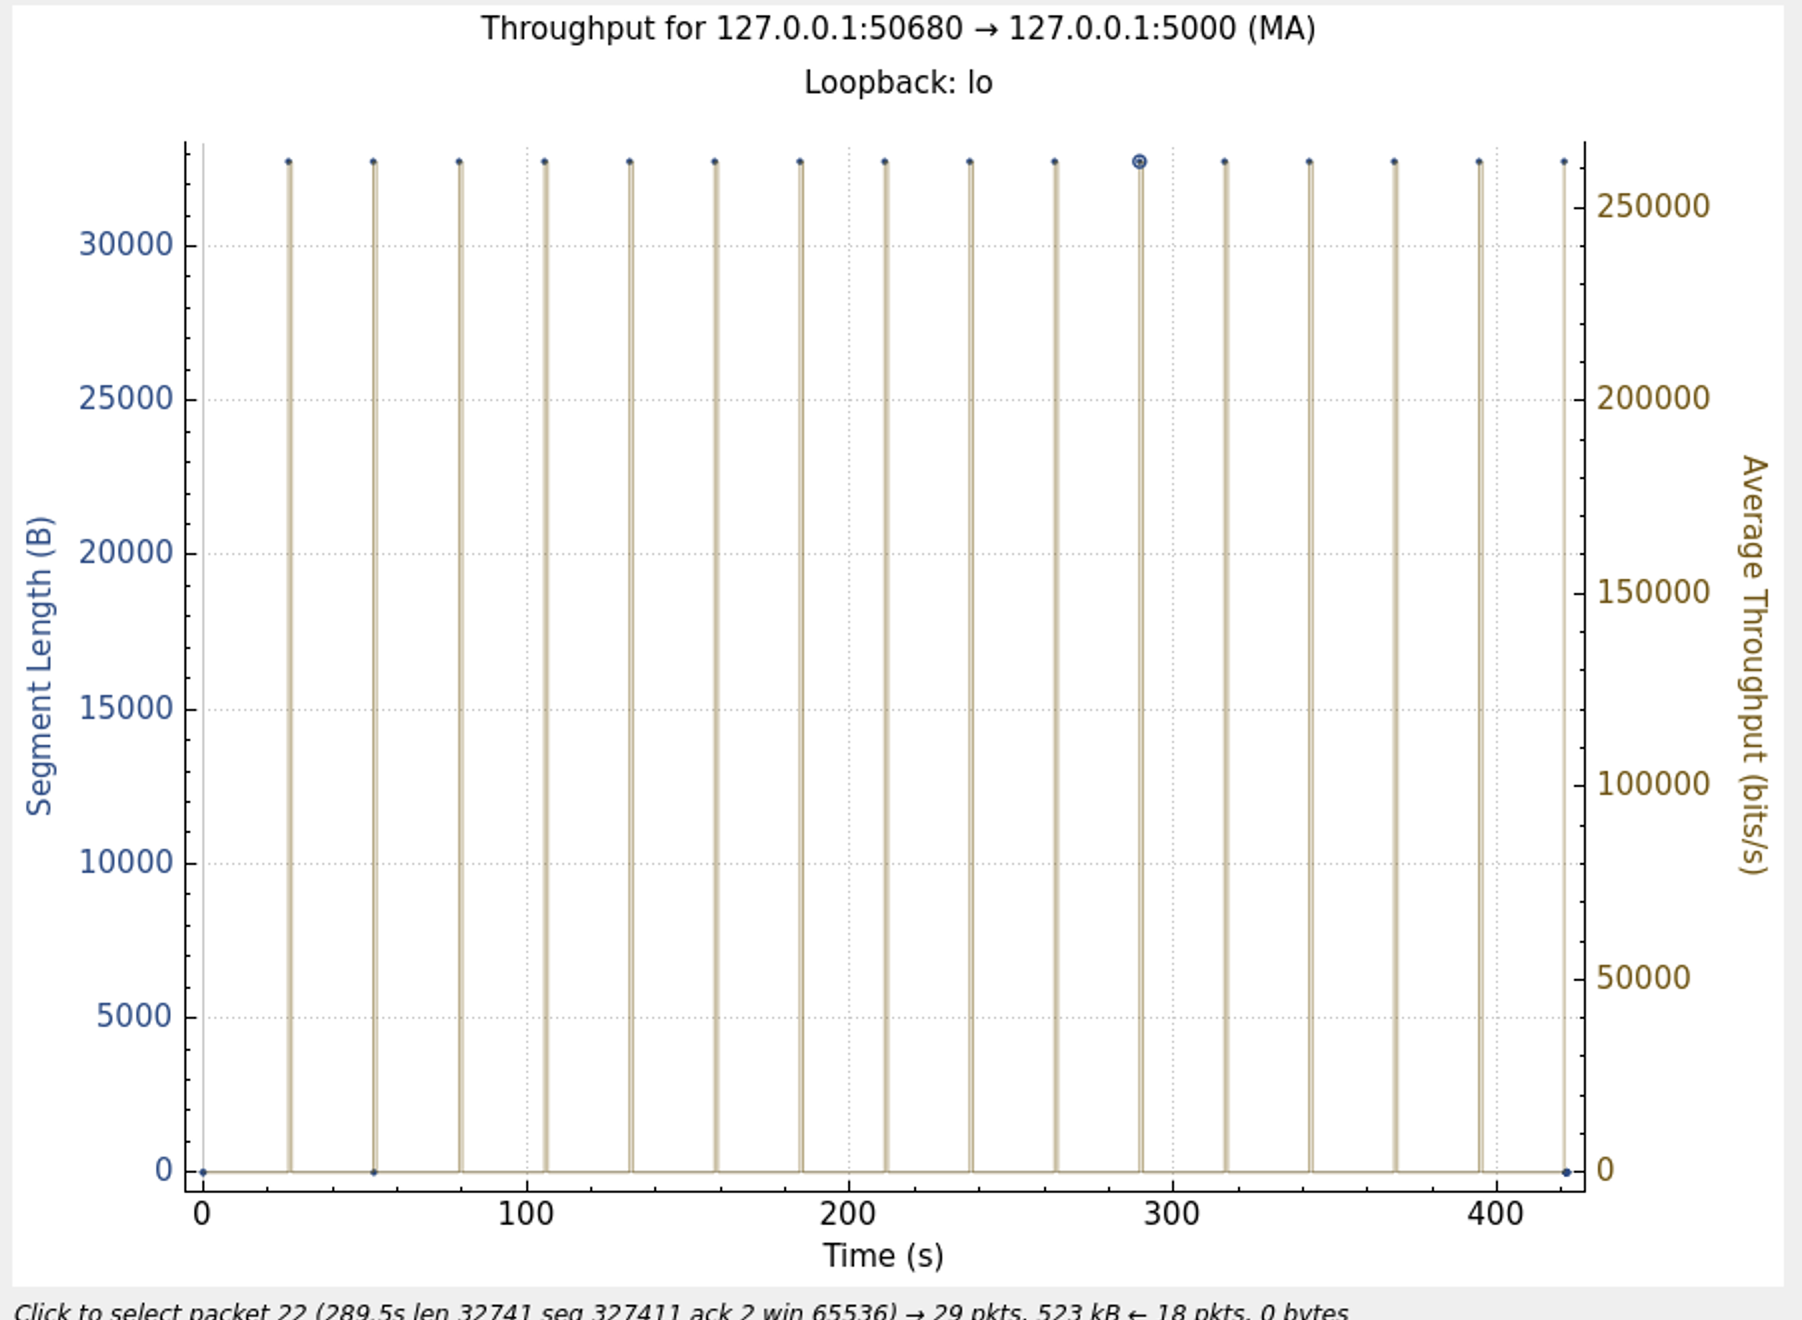
\includegraphics[width=\textwidth]{Pics/Reno/r10kbit_s1m_th}
        \caption{10 kbit rate. BORKED}
    \end{subfigure}
    \caption{Comparison of the throughput for 1mbit of data sent with different rate limits. Reno}
    \label{fig:four_images}
\end{figure}

Comparing figure 9 and figure 5 we can see than with Reno the window scaling has 4 peaks while Cubic had only 3. Also the peaks in Reno seems to reach between 20k and 25k while with cubic they were around 30k.\\
Comparing figure 6b and 10b we can see that Reno has a lower throughput than Cubic. Reno barely breaks the 25k while Cubic almost reaches 30K. Which explains why it felt slower to me during execution.\\
Also as with cubic, sending 1M of data over a rate of 10kb got stuck for a long time after sending about 500k and I had to stop the scripts. This indicate to me a possible issue with my implementation.\\
I didn't notice anything particularly interesting in the round trip times therefore I haven't included any figure with them. They are available on github anyway.

\subsection*{Vegas}
Both Reno and Cubic are congestion algorithms allowed by default in Ubuntu. Vegas on the other hand I had to manually enable. This is important to notice since It isn't beyond me to be so incompetent to make mistakes while enabling it causing some issues.\\
That said given that the command  sysctl net.ipv4.tcp\_allowed\_congestion\_control gives me:\\
\begin{centering}
net.ipv4.tcp\_allowed\_congestion\_control = reno cubic vegas
\end{centering}\\
I will assume to have enabled it correctly.\\
Vegas uses the round trip time to decrease the congestion window to avoid packet loss even before they happen.\\
Comparing figure 11 with figure 9 we can see that the window scaling in pretty similar to Reno. In Vegas as with Reno the window peaks four times at around 20k. On the other hand from figure 12b we can see that the throughput is more similar to Cubic, being slightly lower than 30k.\\
Given that vegas controls its congestion window based on the RTT it is interesting to see that to the four peaks in figure 11C correspond to four peaks in RTT in figure 13C, which shows the RTT of Vegas for different rates with a data size of 1mb. 


\begin{figure}[H]
    \centering
    \begin{subfigure}[b]{0.45\textwidth}
        \centering
        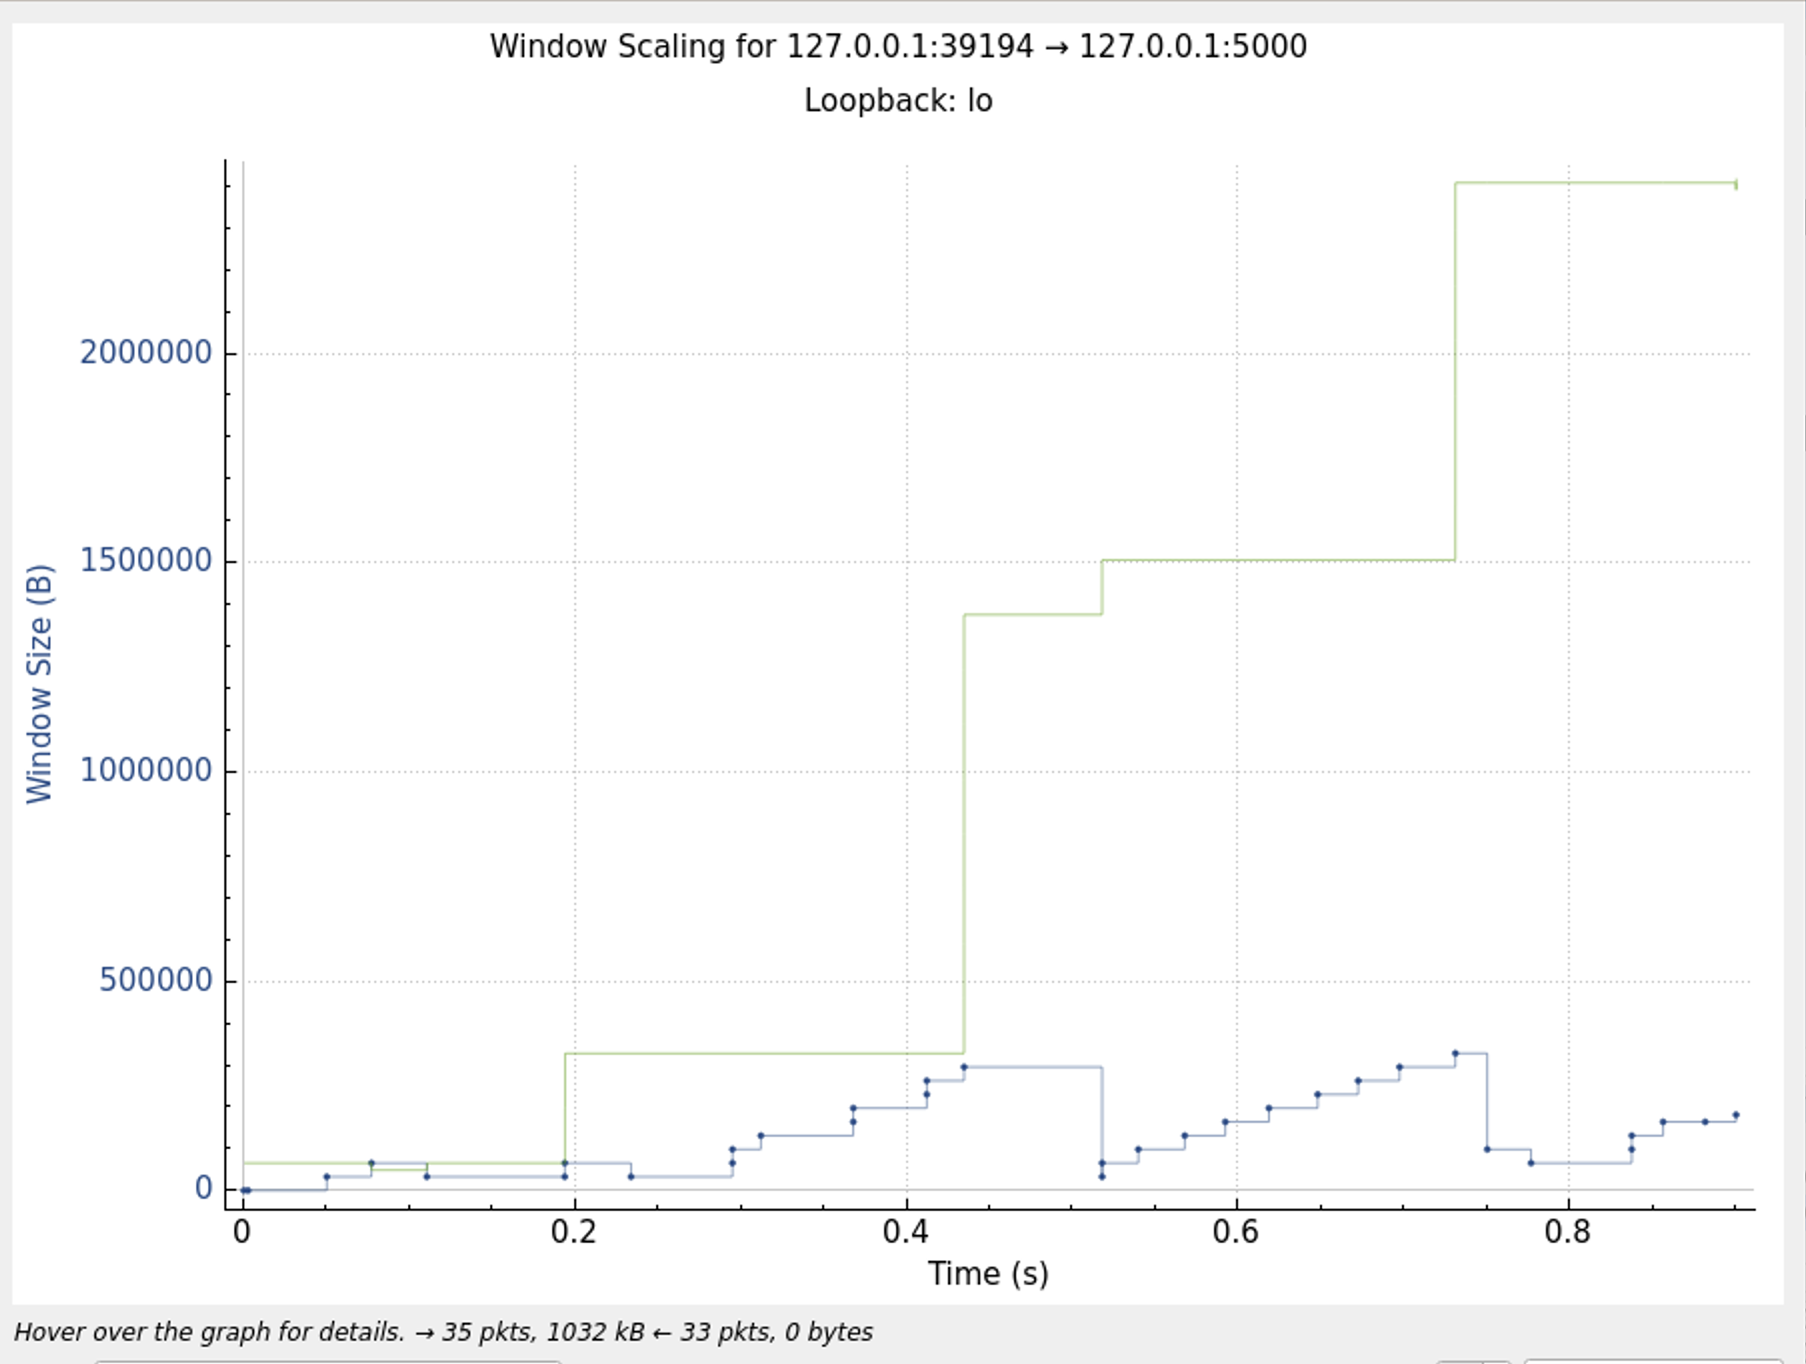
\includegraphics[width=\textwidth]{Pics/Vegas/r10mbit_s1m_ws}
        \caption{10 mbit rate }
    \end{subfigure}
    \hfill
    \begin{subfigure}[b]{0.45\textwidth}
        \centering
        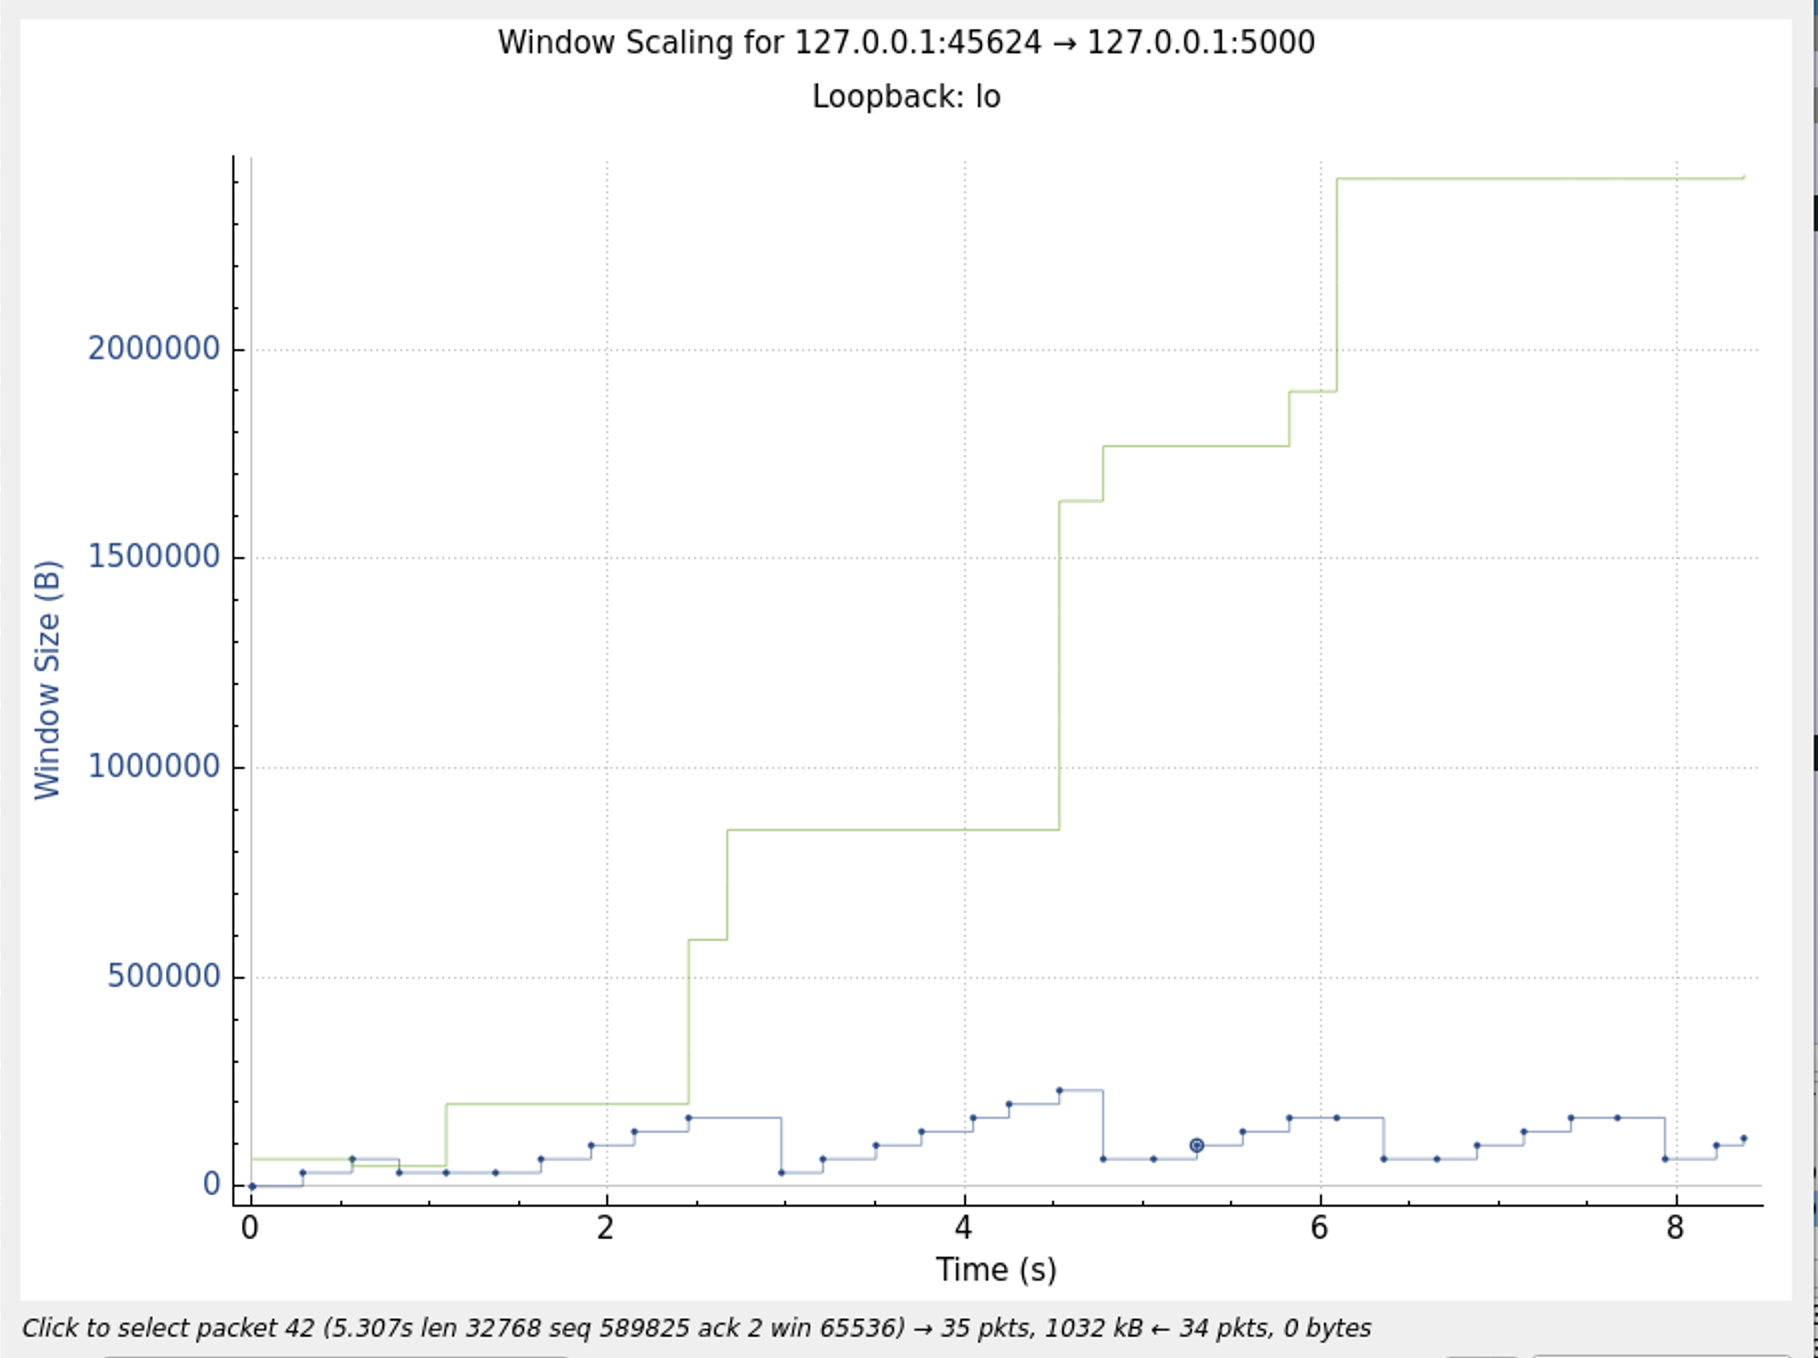
\includegraphics[width=\textwidth]{Pics/Vegas/r1mbit_s1m_ws}
        \caption{1 mbit rate}
    \end{subfigure}
    \medskip

    \begin{subfigure}[b]{0.45\textwidth}
        \centering
        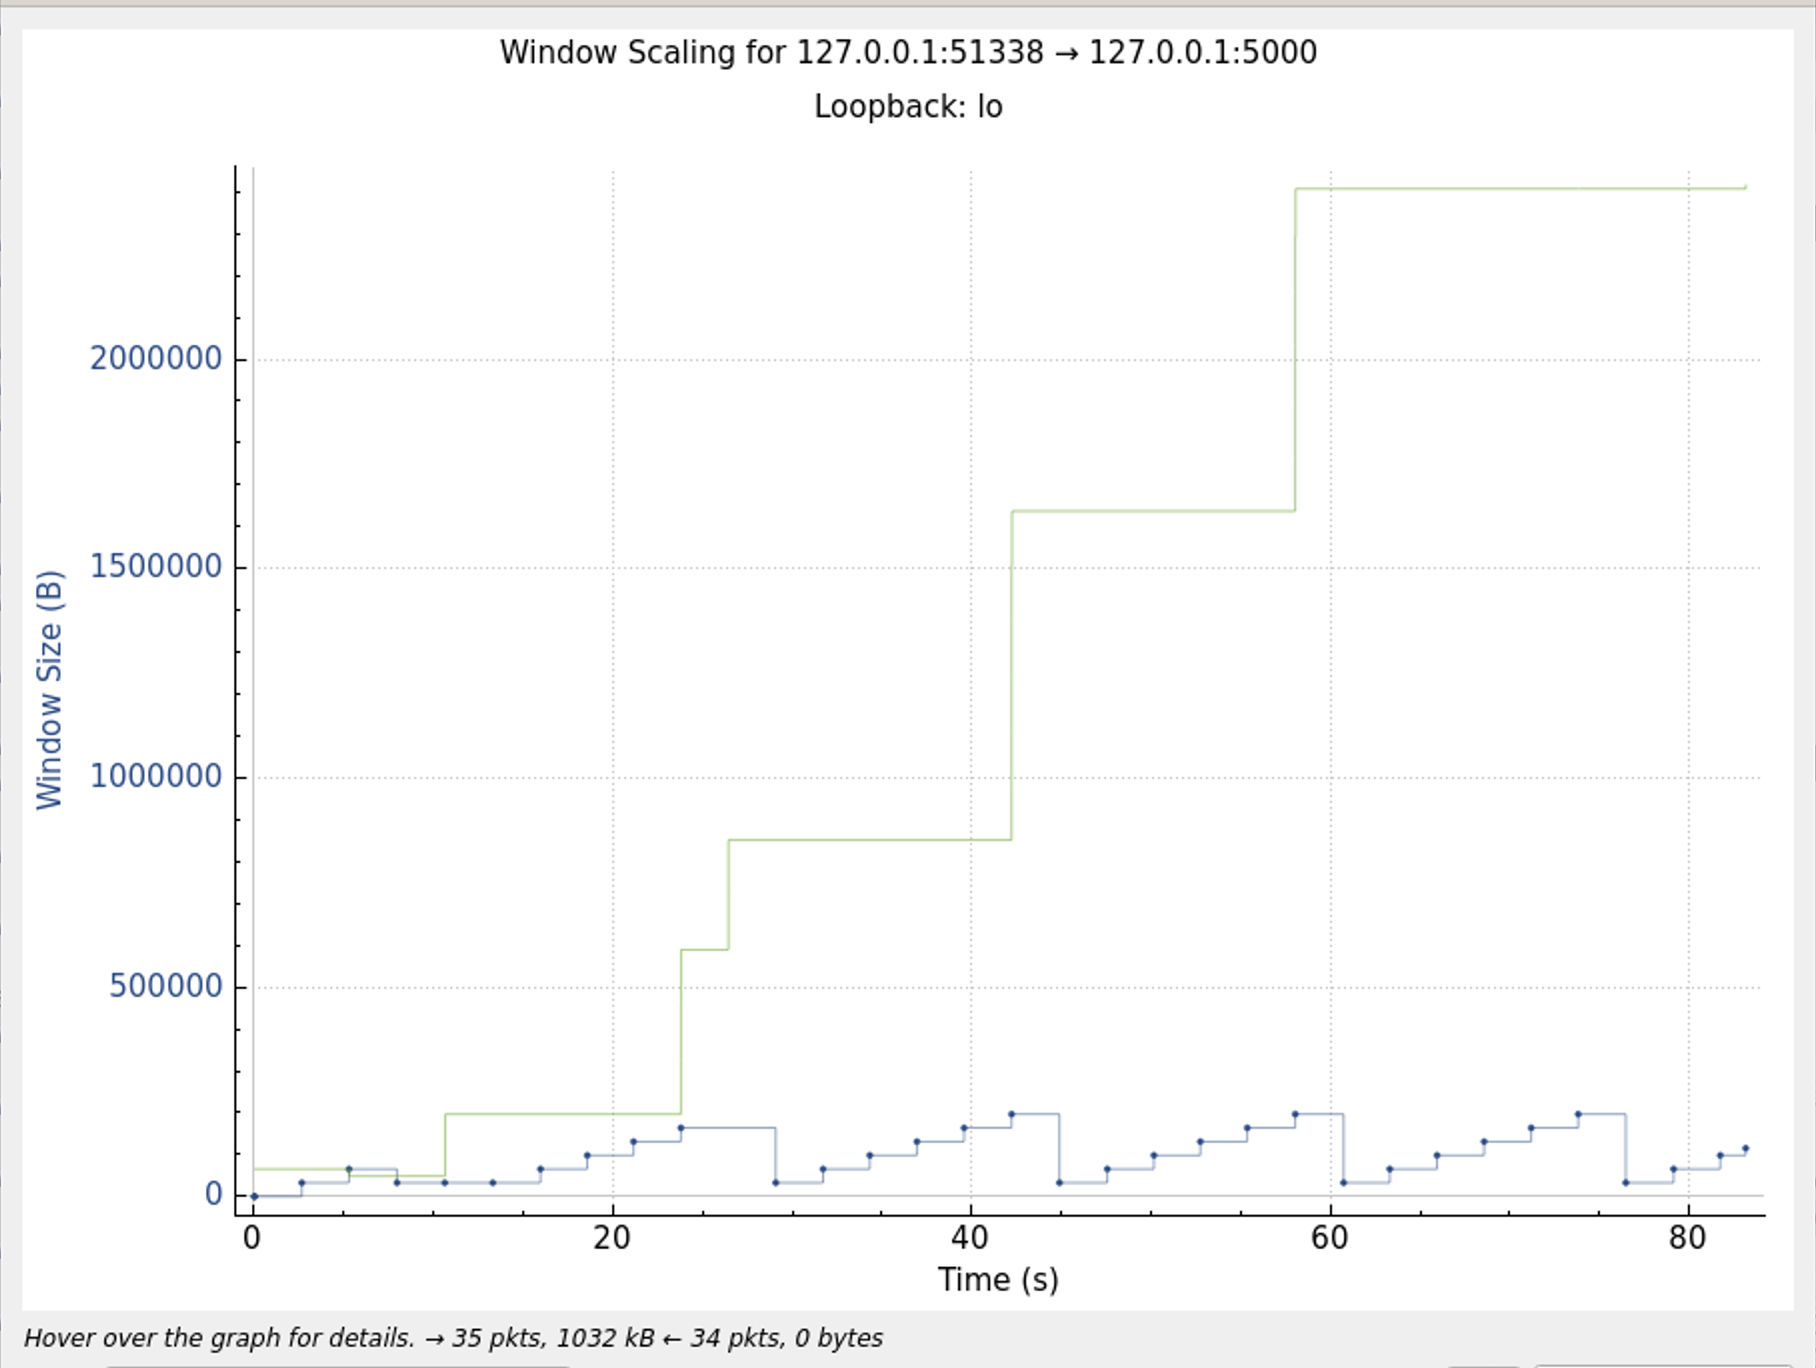
\includegraphics[width=\textwidth]{Pics/Vegas/r100kbit_s1m_ws}
        \caption{100 kbit rate}
    \end{subfigure}
    \hfill
    \begin{subfigure}[b]{0.45\textwidth}
        \centering
        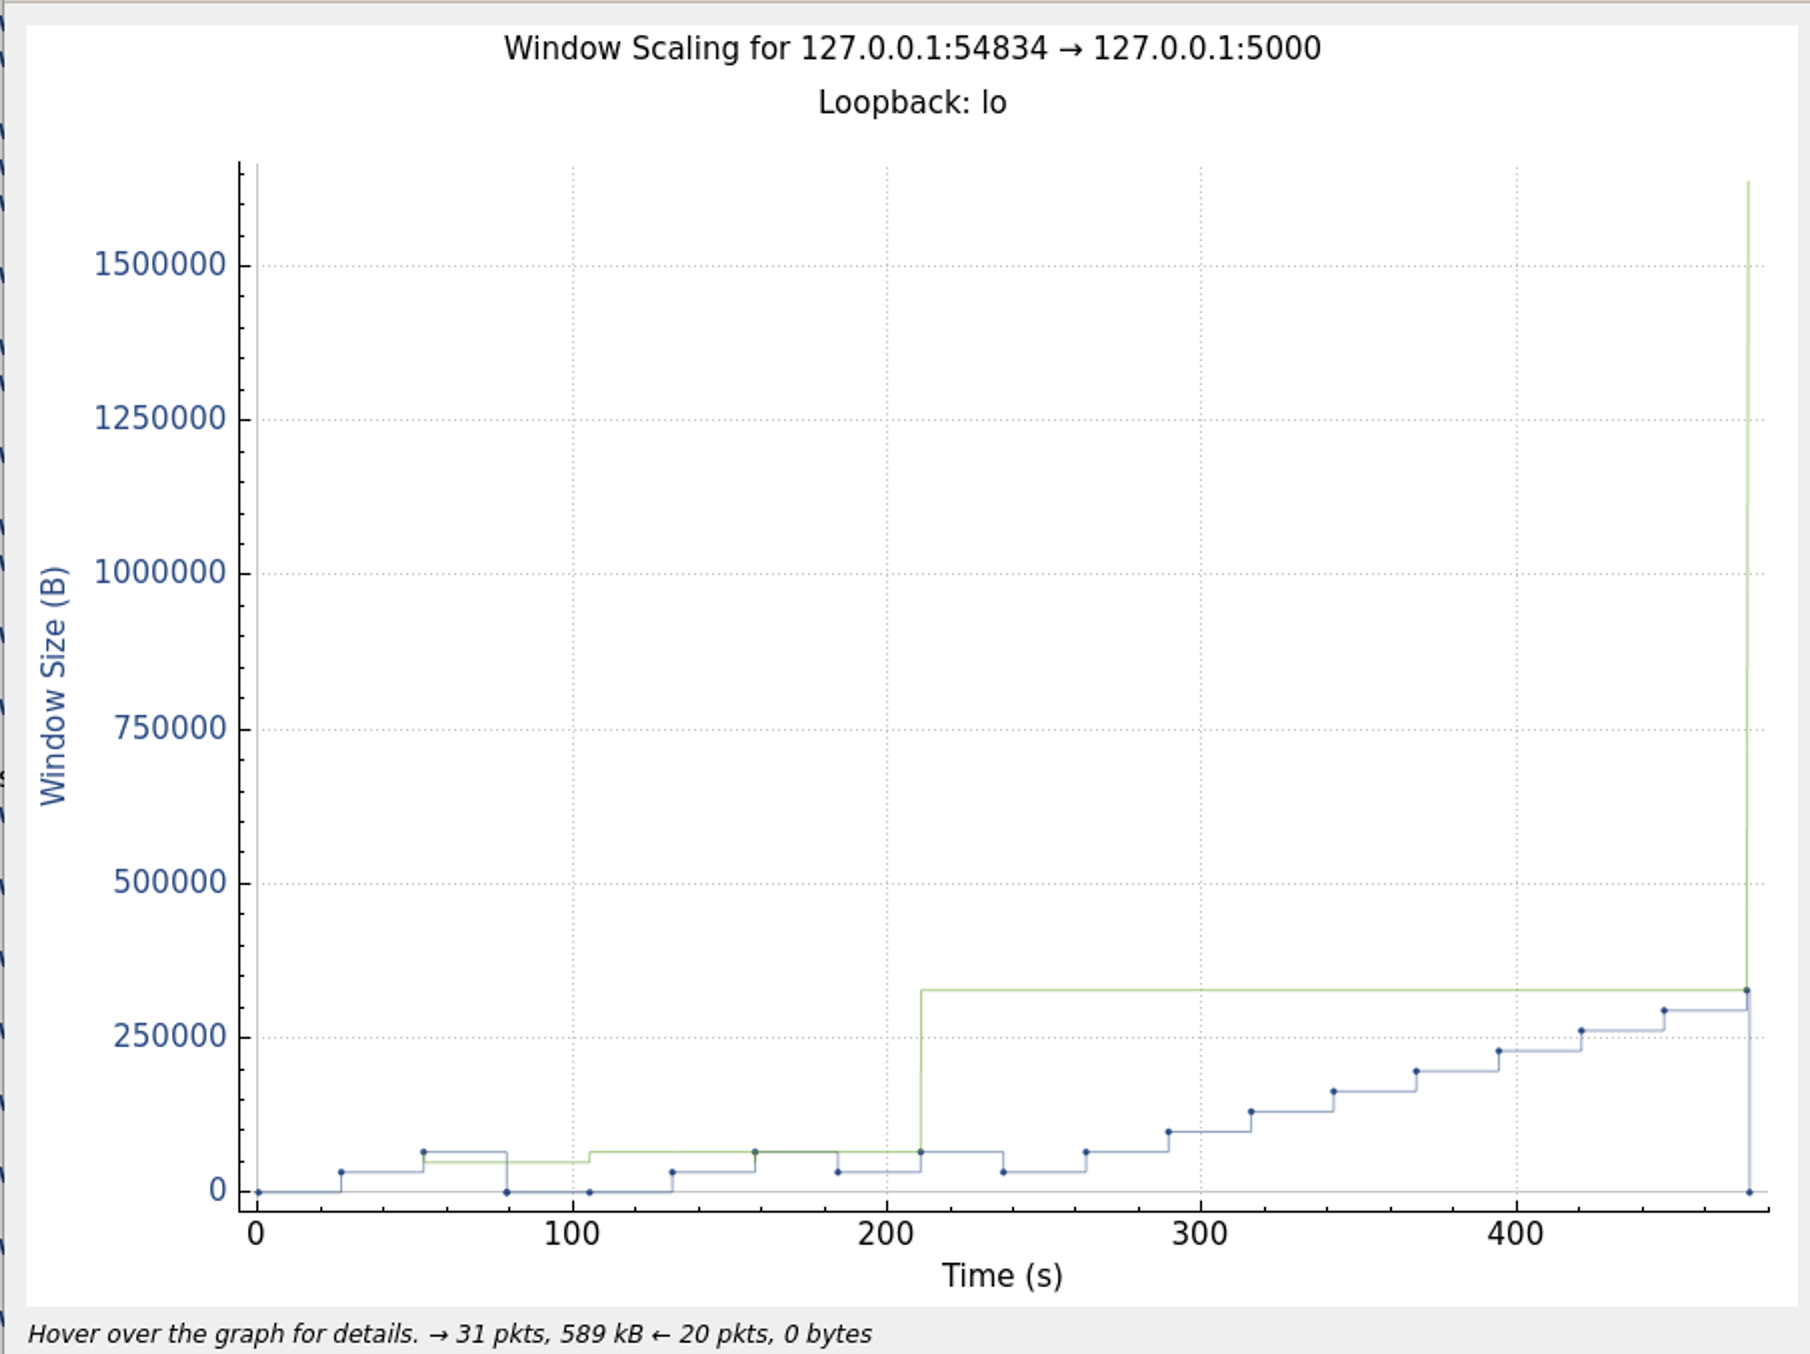
\includegraphics[width=\textwidth]{Pics/Vegas/r10kbit_s1m_ws}
        \caption{10 kbit rate. BORKED}
    \end{subfigure}
    \caption{Comparison of the window scaling for 1mbit of data sent with different rate limits. Vegas}
    \label{fig:four_images}
\end{figure}

\begin{figure}[H]
    \centering
    \begin{subfigure}[b]{0.45\textwidth}
        \centering
        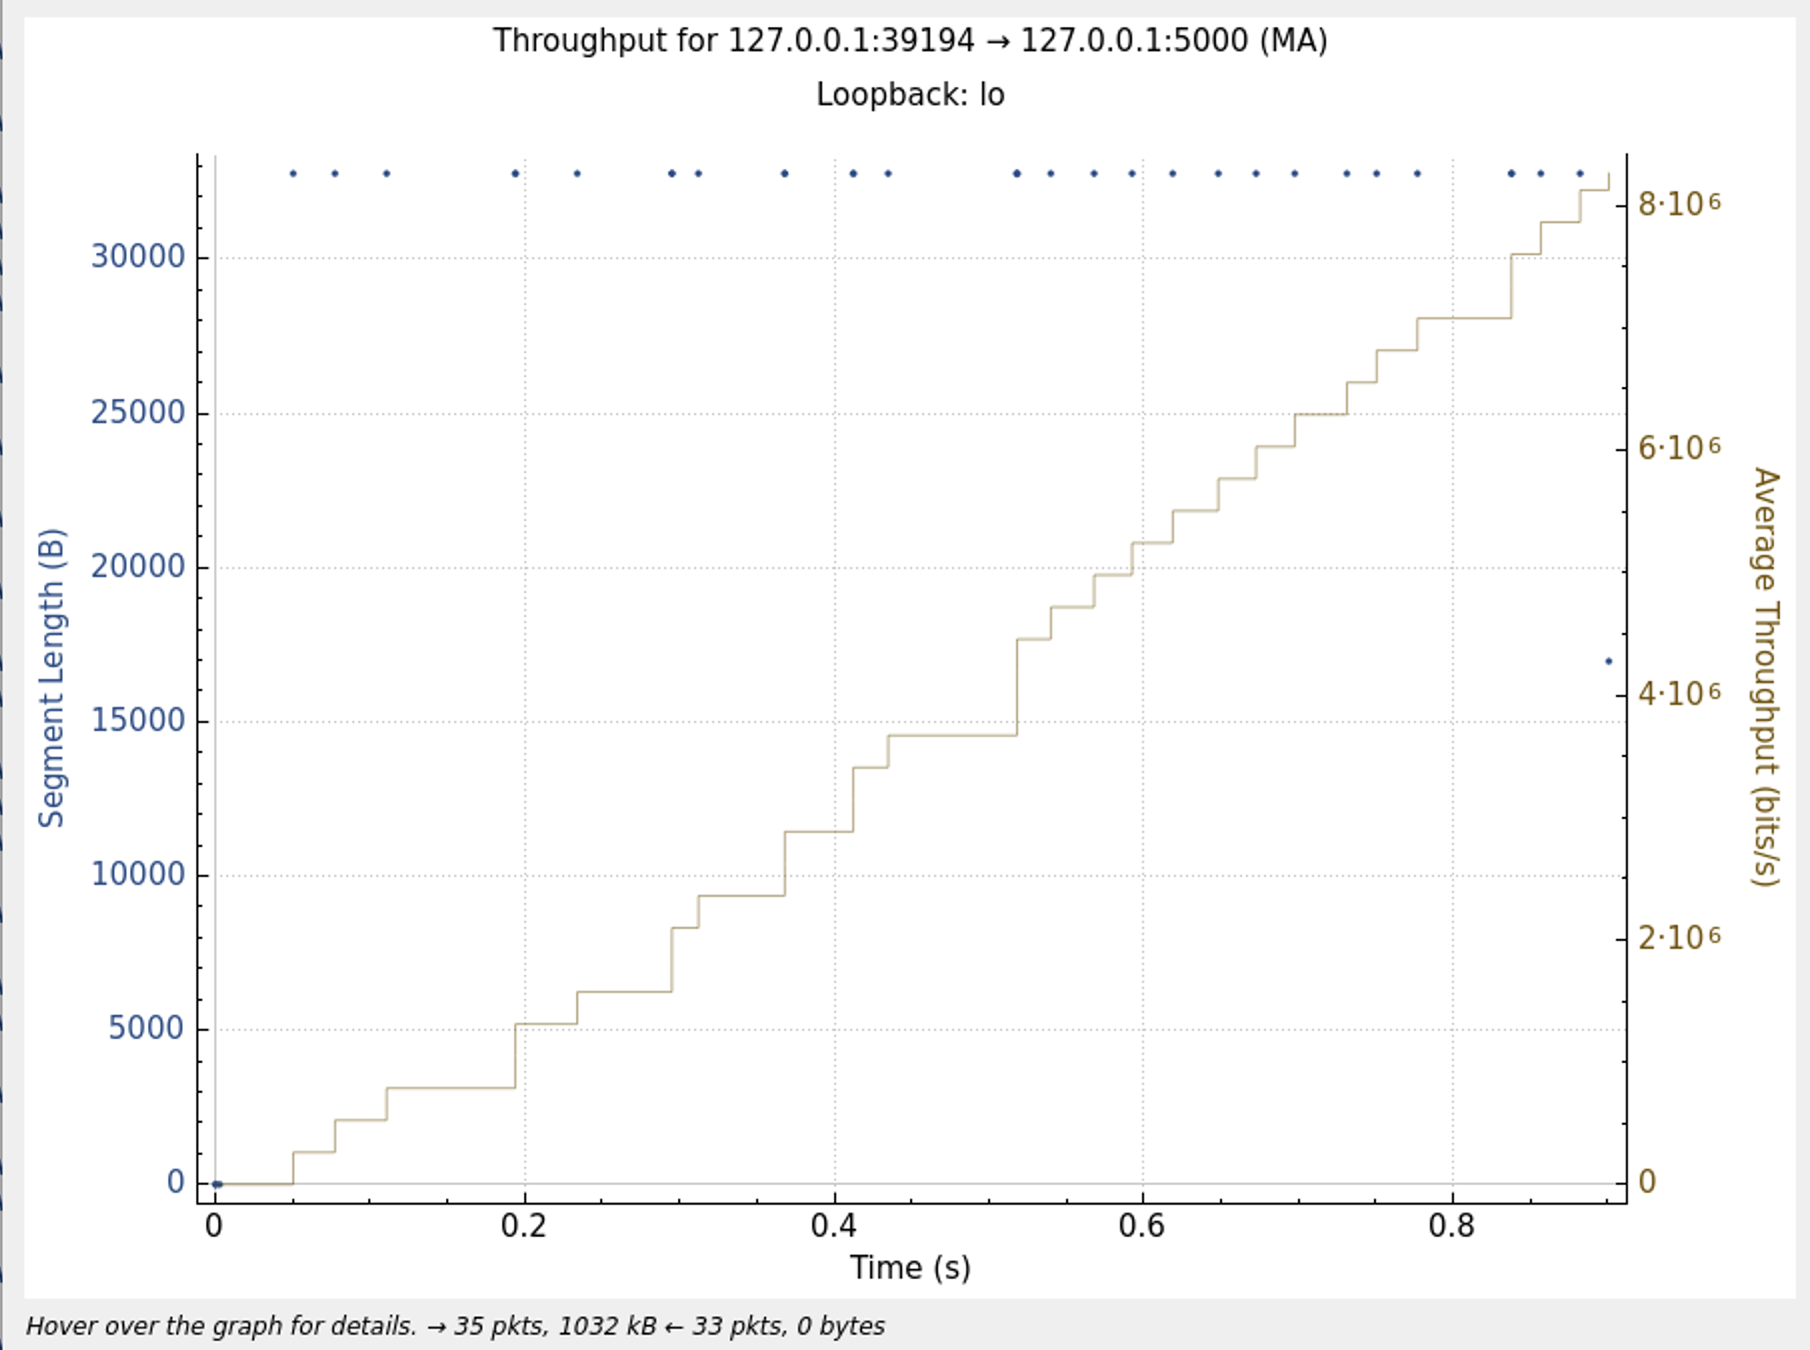
\includegraphics[width=\textwidth]{Pics/Vegas/r10mbit_s1m_th}
        \caption{10 mbit rate}
    \end{subfigure}
    \hfill
    \begin{subfigure}[b]{0.45\textwidth}
        \centering
        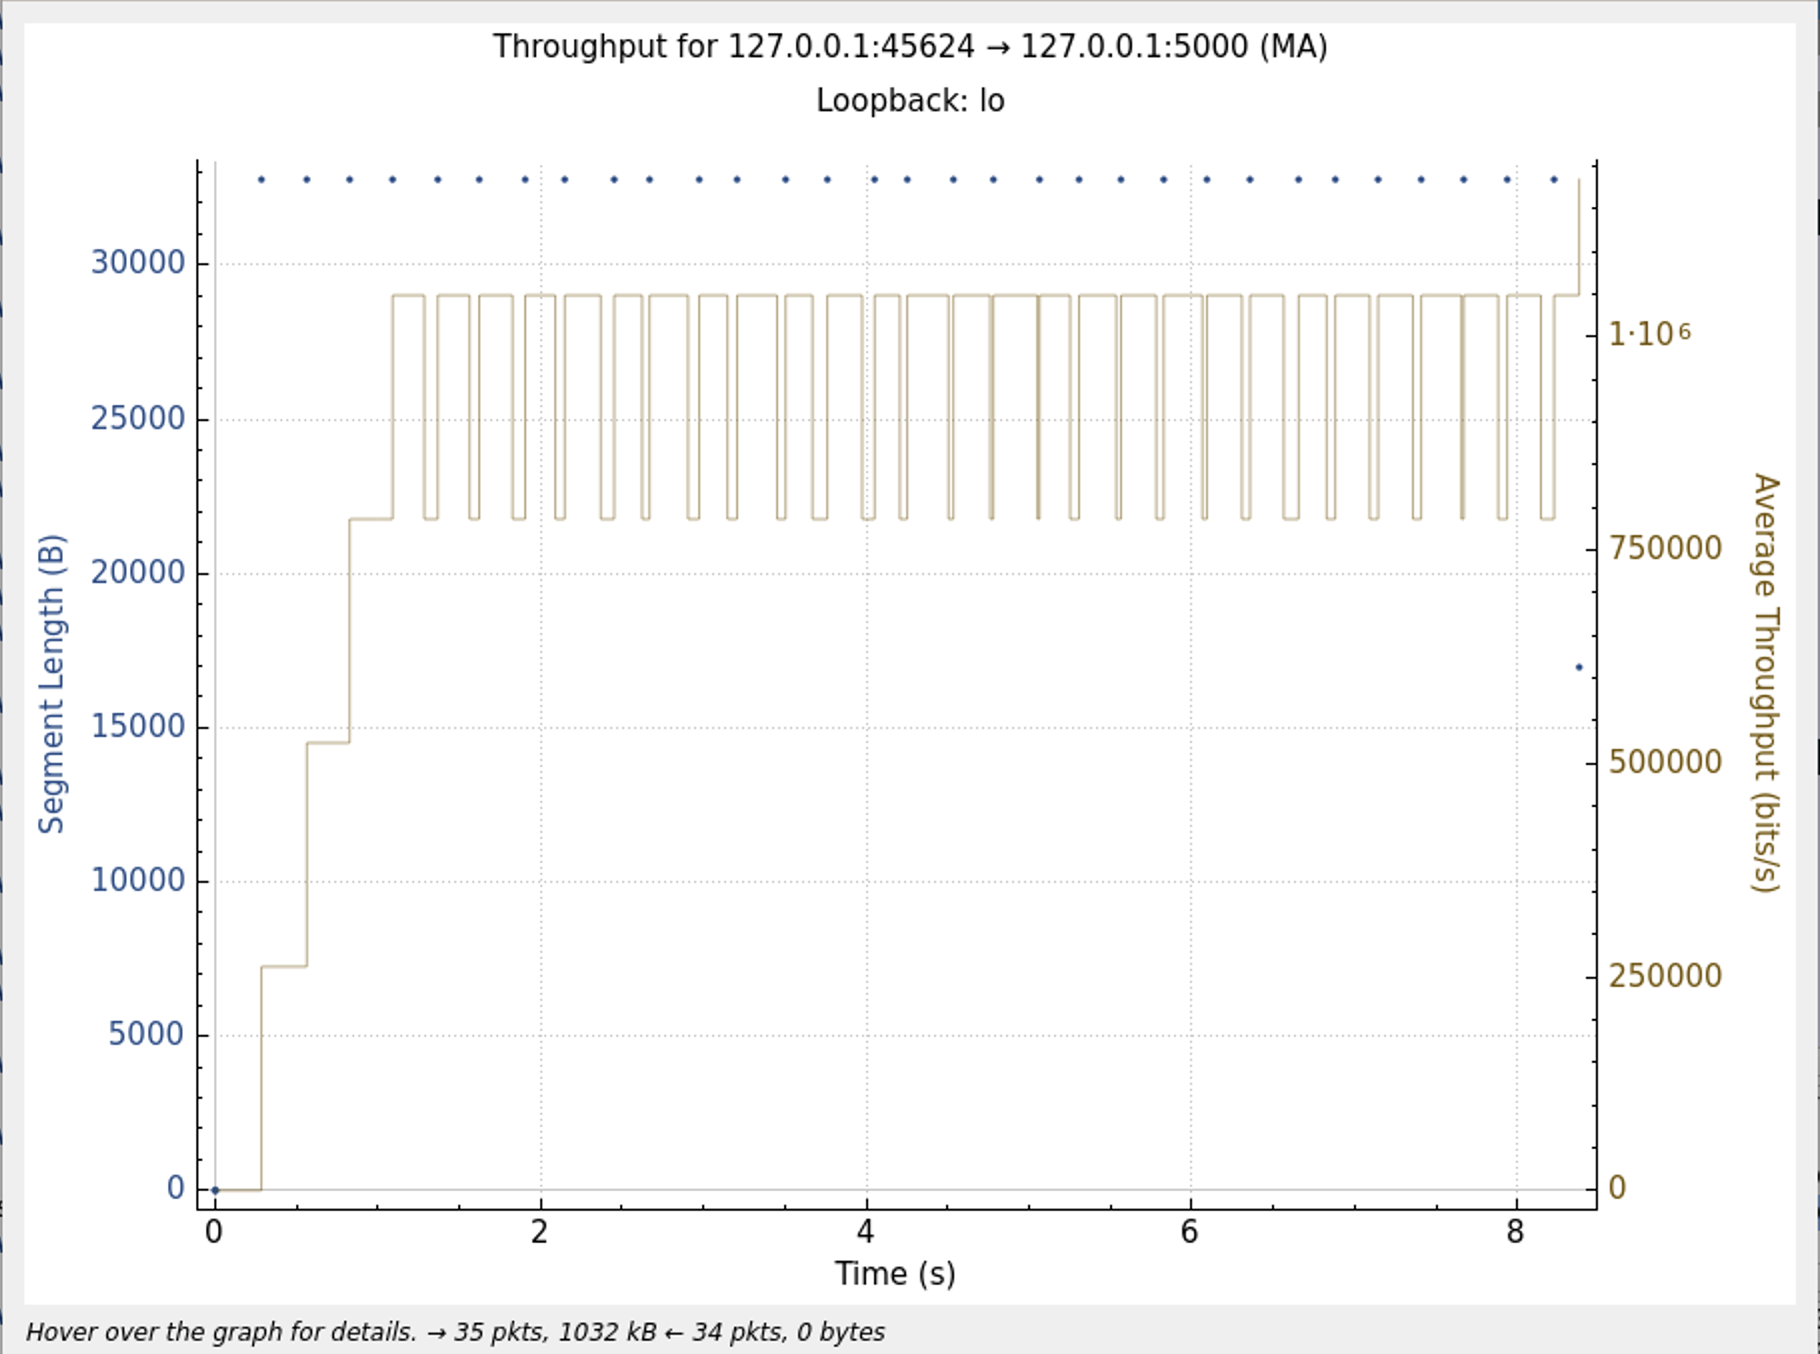
\includegraphics[width=\textwidth]{Pics/Vegas/r1mbit_s1m_th}
        \caption{1 mbit rate}
    \end{subfigure}
    \medskip

    \begin{subfigure}[b]{0.45\textwidth}
        \centering
        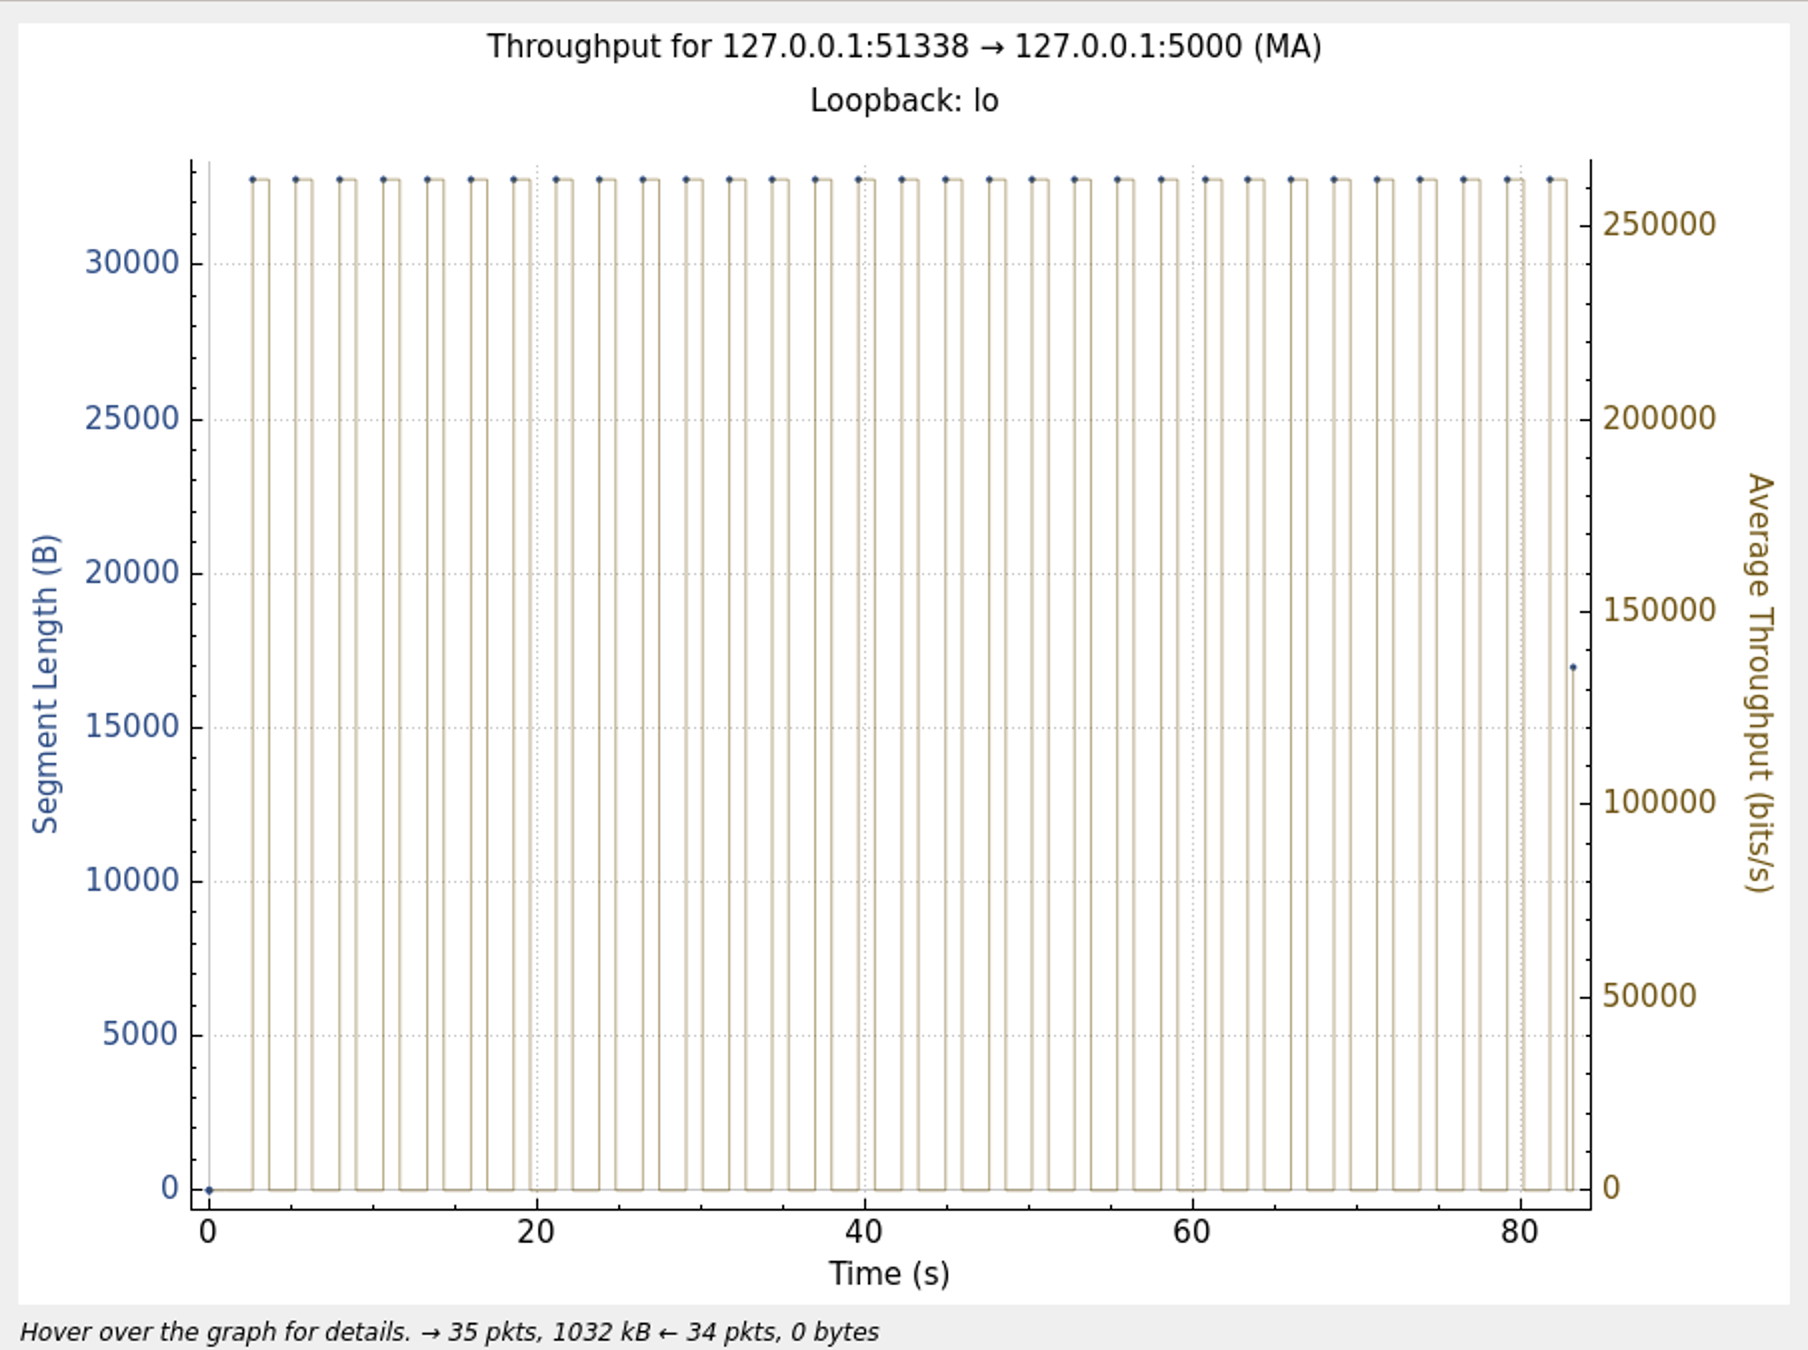
\includegraphics[width=\textwidth]{Pics/Vegas/r100kbit_s1m_th}
        \caption{100 kbit rate}
    \end{subfigure}
    \hfill
    \begin{subfigure}[b]{0.45\textwidth}
        \centering
        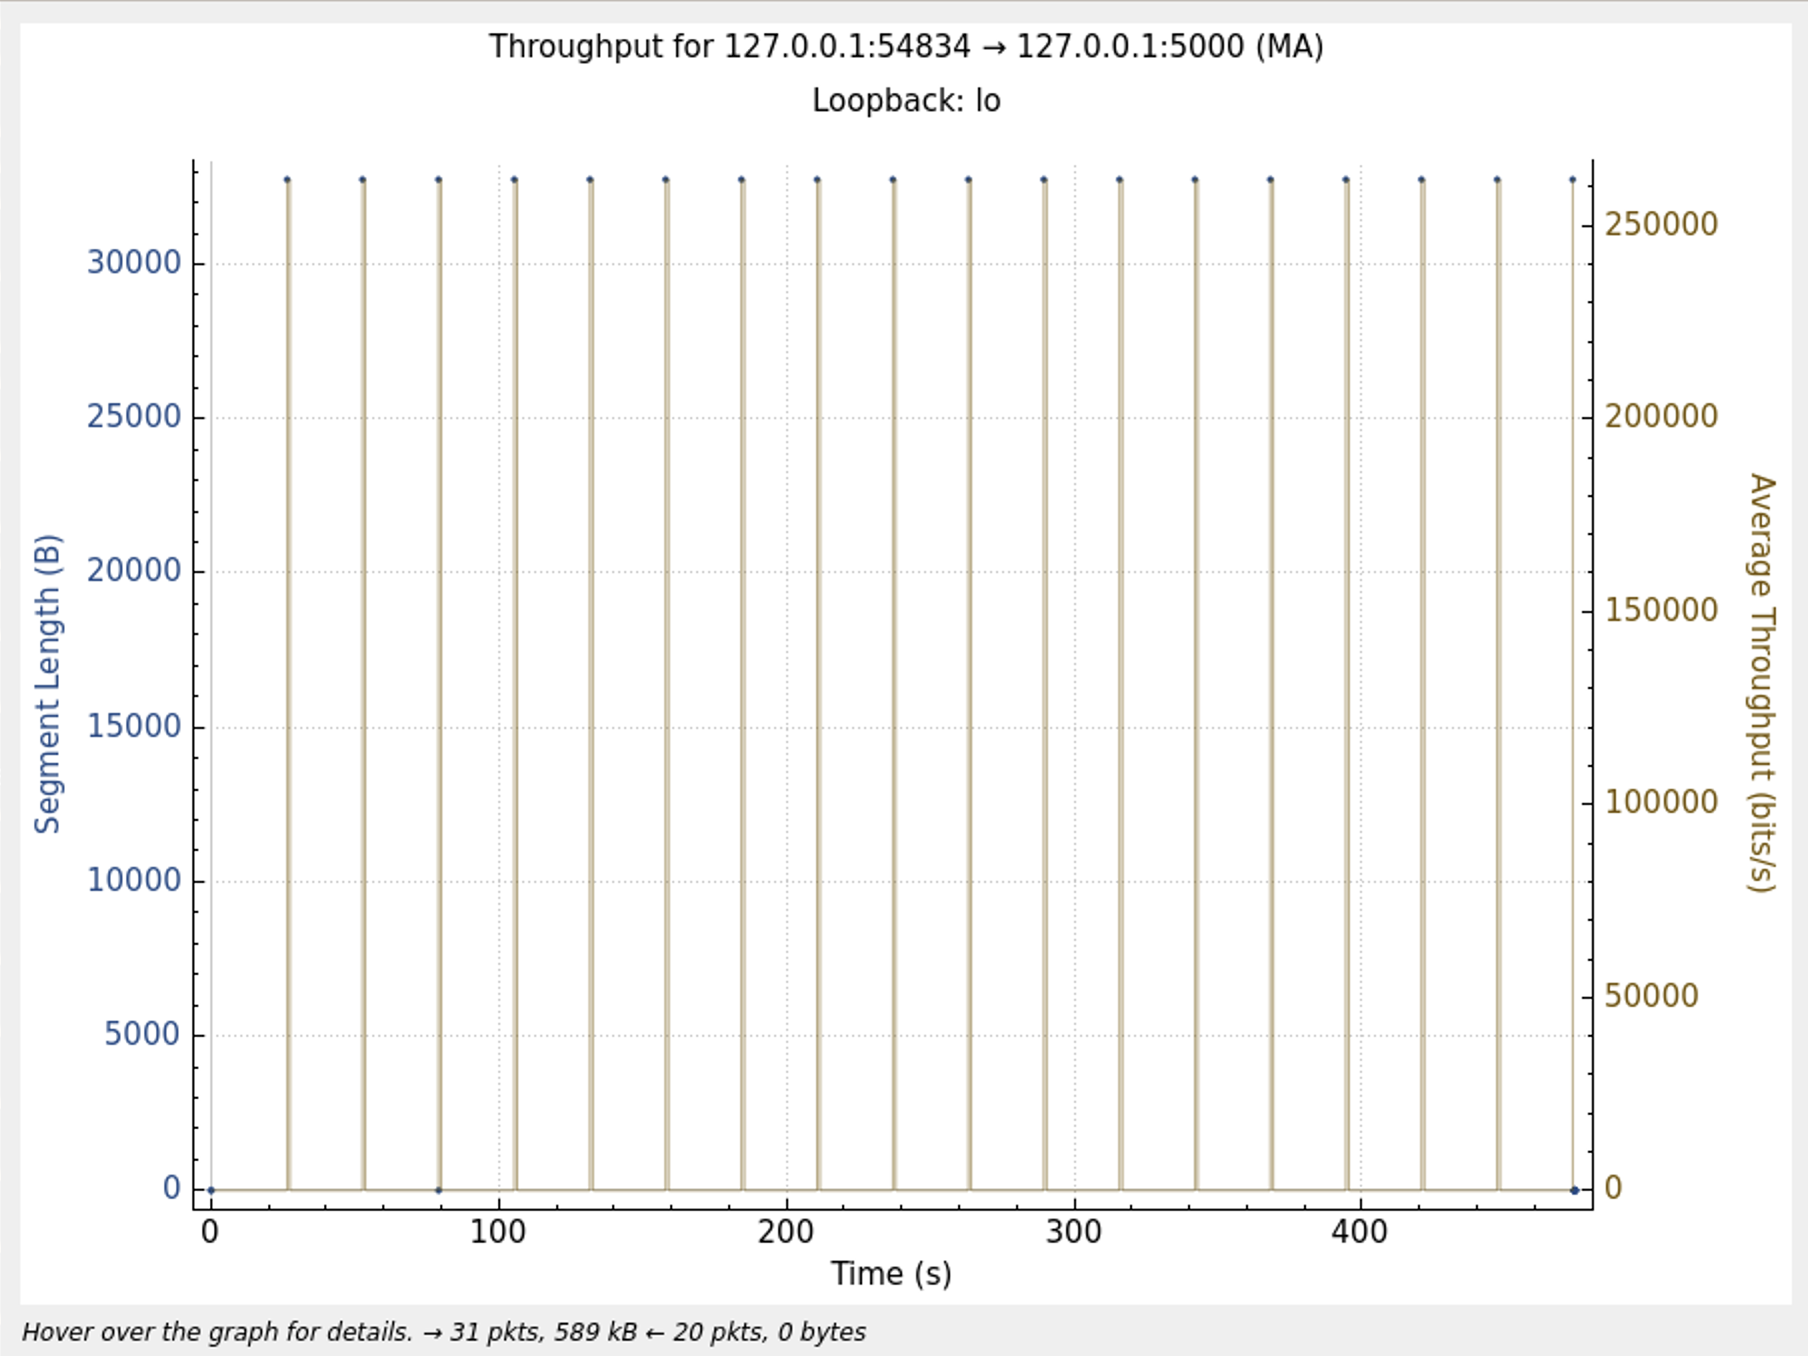
\includegraphics[width=\textwidth]{Pics/Vegas/r10kbit_s1m_th}
        \caption{10 kbit rate. BORKED}
    \end{subfigure}
    \caption{Comparison of the throughput for 1mbit of data sent with different rate limits. Vegas}
    \label{fig:four_images}
\end{figure}

\begin{figure}[H]
    \centering
    \begin{subfigure}[b]{0.45\textwidth}
        \centering
        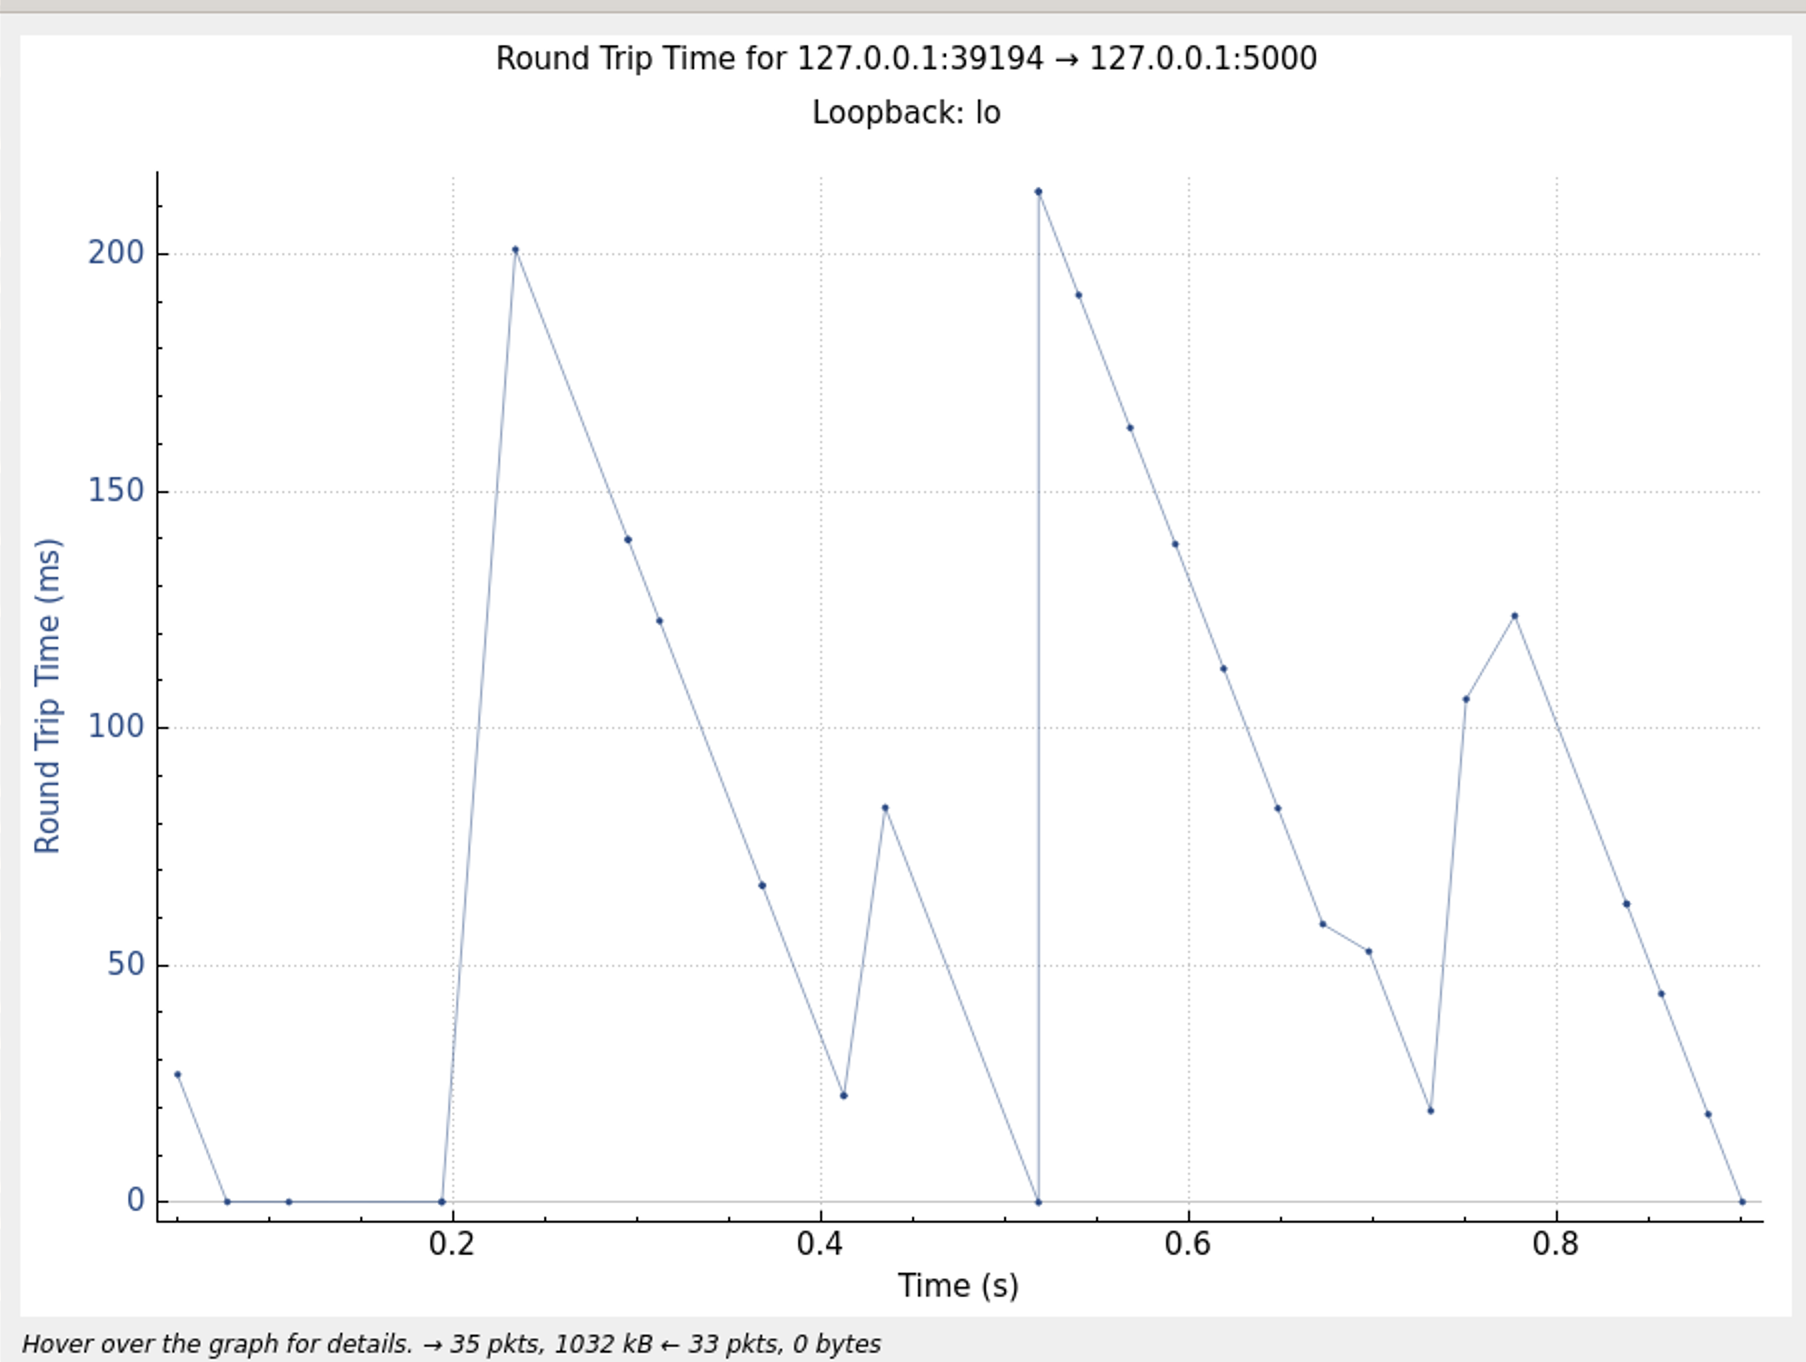
\includegraphics[width=\textwidth]{Pics/Vegas/r10mbit_s1m_rtt}
        \caption{10 mbit rate}
    \end{subfigure}
    \hfill
    \begin{subfigure}[b]{0.45\textwidth}
        \centering
        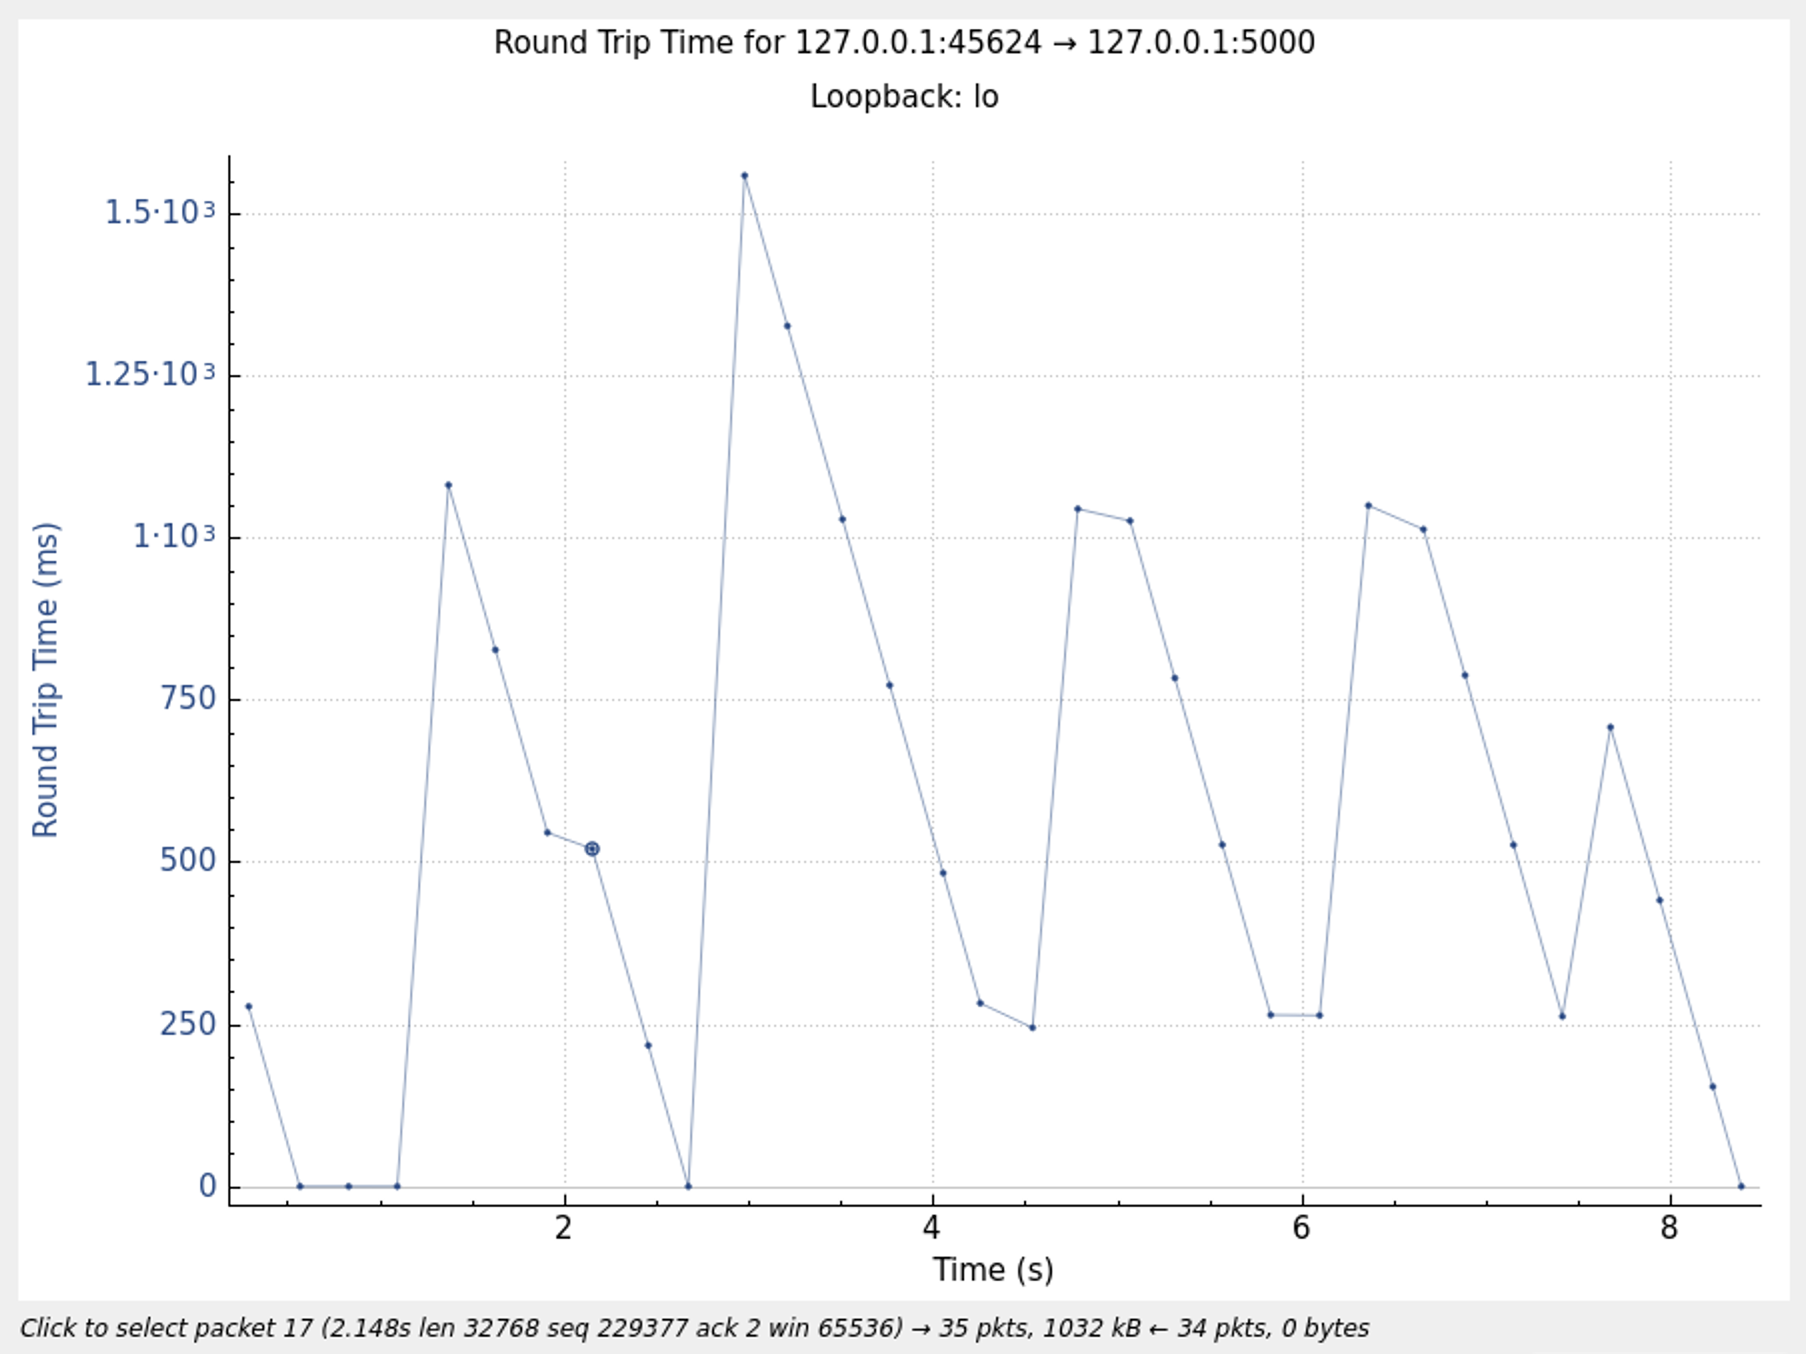
\includegraphics[width=\textwidth]{Pics/Vegas/r1mbit_s1m_rtt}
        \caption{1 mbit rate}
    \end{subfigure}
    \medskip

    \begin{subfigure}[b]{0.45\textwidth}
        \centering
        \includegraphics[width=\textwidth]{Pics/Vegas/r100kbit_s1m_rtt}
        \caption{100 kbit rate}
    \end{subfigure}
    \hfill
    \begin{subfigure}[b]{0.45\textwidth}
        \centering
        \includegraphics[width=\textwidth]{Pics/Vegas/r10kbit_s1m_rtt}
        \caption{10 kbit rate. BORKED}
    \end{subfigure}
    \caption{Comparison of the RTT for 1mbit of data sent with different rate limits. Vegas}
    \label{fig:four_images}
\end{figure}

As with the other two algorithm 1mb on 10kb rate causes some issues.

\subsection*{Westwood}
As for vegas westwood had to be manually enabled. \\
Given the following definition of this algorithm found on wikipedia, I would expect it to perform better than Reno.

\begin{quote}
  TCP Westwood (TCPW) is a sender-side-only modification to TCP New Reno that is intended to better handle large bandwidth-delay product paths (large pipes), with potential packet loss due to transmission or other errors (leaky pipes), and with dynamic load (dynamic pipes).[1]

...

The resultant performance gains in efficiency, without undue sacrifice of fairness, friendliness, and stability have been reported in numerous papers that can be found on The TCP WESTWOOD Home Page. Significant efficiency gains can be obtained for large leaky dynamic pipes, while maintaining fairness. Under a more appropriate criterion for friendliness, i.e. "opportunistic friendliness", TCP Westwood is shown to have good, and controllable, friendliness
  \begin{flushright}
    \tiny{---https://en.wikipedia.org/wiki/TCP\_Westwood}
  \end{flushright}
\end{quote}

Lets observe its throughput and window scaling to get an insight.
\begin{figure}[H]
    \centering
    \begin{subfigure}[b]{0.45\textwidth}
        \centering
        \includegraphics[width=\textwidth]{Pics/Westwood/r10mbit_s1m_ws}
        \caption{10 mbit rate }
    \end{subfigure}
    \hfill
    \begin{subfigure}[b]{0.45\textwidth}
        \centering
        \includegraphics[width=\textwidth]{Pics/Westwood/r1mbit_s1m_ws}
        \caption{1 mbit rate}
    \end{subfigure}
    \medskip

    \begin{subfigure}[b]{0.45\textwidth}
        \centering
        \includegraphics[width=\textwidth]{Pics/Westwood/r100kbit_s1m_ws}
        \caption{100 kbit rate}
    \end{subfigure}
    \hfill
    \begin{subfigure}[b]{0.45\textwidth}
        \centering
        \includegraphics[width=\textwidth]{Pics/Westwood/r10kbit_s1m_ws}
        \caption{10 kbit rate. BORKED}
    \end{subfigure}
    \caption{Comparison of the window scaling for 1mbit of data sent with different rate limits. Westwood}
    \label{fig:four_images}
\end{figure}

\begin{figure}[H]
    \centering
    \begin{subfigure}[b]{0.45\textwidth}
        \centering
        \includegraphics[width=\textwidth]{Pics/Westwood/r10mbit_s1m_th}
        \caption{10 mbit rate}
    \end{subfigure}
    \hfill
    \begin{subfigure}[b]{0.45\textwidth}
        \centering
        \includegraphics[width=\textwidth]{Pics/Westwood/r1mbit_s1m_th}
        \caption{1 mbit rate}
    \end{subfigure}
    \medskip

    \begin{subfigure}[b]{0.45\textwidth}
        \centering
        \includegraphics[width=\textwidth]{Pics/Westwood/r100kbit_s1m_th}
        \caption{100 kbit rate}
    \end{subfigure}
    \hfill
    \begin{subfigure}[b]{0.45\textwidth}
        \centering
        \includegraphics[width=\textwidth]{Pics/Westwood/r10kbit_s1m_th}
        \caption{10 kbit rate. BORKED}
    \end{subfigure}
    \caption{Comparison of the throughput for 1mbit of data sent with different rate limits. Westwood}
    \label{fig:four_images}
\end{figure}
Comparing figure 14b to figure 9b I  find them to be pretty similar, both peaking at a window of roughly 20K. Interestingly the window scaling in figure 14 c only has two big peaks, of roughly 30K, and a smaller one, of roughly 20K, while we can see in figure 9C that Reno had 4 more consistent peaks at roughly 20K.\\
Figure 15b and 10b also showcase a similar throughput. The improvement in performance which westwood should have does not seem to be evident with my limited experiment.

\subsection*{Comparison}
Given all of the data gathered about these congestion control algorithms it only makes sense to compare and contrast them.\\
This comparison will be based on the 1 mbit of data send at a rate limited to 1mb. I think it became clear from the previous experimentation that the more data is sent the easier is to see scaling and shrinking of the congestion window. Regarding the rate, at rates which are to low  I don't believe that the differences in throughput between algorithms are clear.\\
\begin{figure}[H]
    \centering
    \begin{subfigure}[b]{0.45\textwidth}
        \centering
        \includegraphics[width=\textwidth]{Pics/Cubic/r1mbit_s1m_th}
        \caption{Cubic}
    \end{subfigure}
    \hfill
    \begin{subfigure}[b]{0.45\textwidth}
        \centering
        \includegraphics[width=\textwidth]{Pics/Reno/r1mbit_s1m_th}
        \caption{Reno}
    \end{subfigure}
    \medskip

    \begin{subfigure}[b]{0.45\textwidth}
        \centering
        \includegraphics[width=\textwidth]{Pics/Vegas/r1mbit_s1m_th}
        \caption{Vegas}
    \end{subfigure}
    \hfill
    \begin{subfigure}[b]{0.45\textwidth}
        \centering
        \includegraphics[width=\textwidth]{Pics/Westwood/r1mbit_s1m_th}
        \caption{Westwood}
    \end{subfigure}
    \caption{Comparison of the throughput for 1mbit of data sent at a rate limited to 1mb.}
    \label{fig:four_images}
\end{figure}

\begin{figure}[H]
    \centering
    \begin{subfigure}[b]{0.45\textwidth}
        \centering
        \includegraphics[width=\textwidth]{Pics/Cubic/r1mbit_s1m_rtt}
        \caption{Cubic}
    \end{subfigure}
    \hfill
    \begin{subfigure}[b]{0.45\textwidth}
        \centering
        \includegraphics[width=\textwidth]{Pics/Reno/r1mbit_s1m_rtt}
        \caption{Reno}
    \end{subfigure}
    \medskip

    \begin{subfigure}[b]{0.45\textwidth}
        \centering
        \includegraphics[width=\textwidth]{Pics/Vegas/r1mbit_s1m_rtt}
        \caption{Vegas}
    \end{subfigure}
    \hfill
    \begin{subfigure}[b]{0.45\textwidth}
        \centering
        \includegraphics[width=\textwidth]{Pics/Westwood/r1mbit_s1m_rtt}
        \caption{Westwood}
    \end{subfigure}
    \caption{Comparison of the round trip time for 1mbit of data sent at a rate limited to 1mb.}
    \label{fig:four_images}
\end{figure}

\begin{figure}[H]
    \centering
    \begin{subfigure}[b]{0.45\textwidth}
        \centering
        \includegraphics[width=\textwidth]{Pics/Cubic/r1mbit_s1m_ws}
        \caption{Cubic}
    \end{subfigure}
    \hfill
    \begin{subfigure}[b]{0.45\textwidth}
        \centering
        \includegraphics[width=\textwidth]{Pics/Reno/r1mbit_s1m_ws}
        \caption{Reno}
    \end{subfigure}
    \medskip

    \begin{subfigure}[b]{0.45\textwidth}
        \centering
        \includegraphics[width=\textwidth]{Pics/Vegas/r1mbit_s1m_ws}
        \caption{Vegas}
    \end{subfigure}
    \hfill
    \begin{subfigure}[b]{0.45\textwidth}
        \centering
        \includegraphics[width=\textwidth]{Pics/Westwood/r1mbit_s1m_ws}
        \caption{Westwood}
    \end{subfigure}
    \caption{Comparison of the window scaling for 1mbit of data sent at a rate limited to 1mb.}
    \label{fig:four_images}
\end{figure}

From figure 16 it is clear that Cubic and Vegas have comparable throughput, Reno and Westwood also have a similar throughput and Cubic/Vegas throughput is higher on average than Reno/Westwood.\\
Regarding the round trip time, observable in figure 17, I find more difficult to analyse. That said Cubic and Reno seems to have higher peaks of RTT with respect to Vegas and westwood. Vegas seems to keep it below, or just higher than 1 second (beside one peak) and Westwood keeps the RTT low but with some high peaks.\\
From figure 18 we can see that Cubic has fewer seats back, 3, with respects to other algorithms and it seem to peak at a higher window size. I don't seem to find major differences among to other three algorithms.


\section*{Issues}
The rate limiter script begins with a shebang to /bin/sh, on ubuntu this is a symlink to dash. This leads to an issue since the 'function' keyword is not valid in dash but only in bash. To fix this issue I have changed the shebang to \#!/bin/bash.\\
Another issue, as discussed previously is the fact that with a rate limited to 10kbit and a data sent size of 1mbit, with all algorithm there were problems. I am not sure why this would be the case.



\end{document}